% =====================================================================
% Master's Thesis -- master document
% Wires the abstract plus five chapter files (ch0_abstract, ch1 .. ch5) into one
% FPT-template report-class PDF. Build from THIS directory:
%     latexmk -pdf main.tex
% (or: pdflatex main; bibtex main; pdflatex main; pdflatex main)
%
% Each ch*.tex is a body FRAGMENT (no preamble, no \begin/\end{document});
% top-level headings were promoted \section->\chapter, \subsection->\section,
% \subsubsection->\subsection at assembly. Cross-chapter references are real
% \ref{} into the shared label namespace this file creates.
% =====================================================================
\documentclass[a4paper,12pt]{report}

% --- Base packages (union of every fragment + the FPT template) ---
\usepackage[english]{babel}
\usepackage{indentfirst}  % indent the first paragraph after every heading too
\usepackage[utf8]{inputenc}
\usepackage[T1]{fontenc}
\usepackage{lmodern}
\usepackage{amsmath,amssymb,amsfonts}
\usepackage{bm}
\usepackage{booktabs}
\usepackage{float}
\usepackage{siunitx}
\usepackage{microtype}
\usepackage{graphicx}
\usepackage{multirow}
\usepackage{array}
\usepackage{url}
\usepackage[super]{nth}
\usepackage[margin=2.5cm]{geometry}
\usepackage{fancyhdr}

% --- Chapter 3 pipeline diagram ---
\usepackage{tikz}
\usetikzlibrary{arrows.meta,positioning,fit,backgrounds,calc,shapes.geometric}

% --- Custom siunitx units used in the timing tables/figures (Ch 3-4) ---
% (\frame is otherwise the LaTeX kernel box-frame command, not a unit.)
\DeclareSIUnit{\frame}{frame}
\DeclareSIUnit{\fps}{fps}

% --- Figures ---
% Committed copies live in figures/ (tracked, so the thesis builds from a plain
% clone on any machine). The gitignored output/ tree is kept as a fallback so a
% freshly regenerated figure is still picked up on the authoring machine.
% Paths are relative to this master in docs/writing/thesis/.
\graphicspath{{figures/}{../../../output/figures/}{../../../output/experiments/}}

% --- Header / footer (FPT template style) ---
\setlength{\headheight}{15pt}
\addtolength{\topmargin}{-3pt}
\pagestyle{fancy}
\fancyhf{}
\lhead{FPT School of Business \& Technology}
\cfoot{\thepage}
\renewcommand{\headrulewidth}{0.5pt}
\renewcommand{\footrulewidth}{0.5pt}

\begin{document}
\sloppy

% --- Title page (FPT template style) ---
\begin{titlepage}
  \begin{center}
    
\includegraphics[scale=0.3]{../report-template/Images/fpt.png}
  \end{center}

  \center
  \vspace{0.5in}
  \textbf{\large MASTER'S THESIS}
  \vspace{0.5in}

  \noindent\makebox[\linewidth]{\rule{\linewidth}{1.2pt}}
  \textbf{\large A Modular Detection and Completion Framework for
    Occluded Vehicles in Automotive LiDAR}
  \noindent\makebox[\linewidth]{\rule{\linewidth}{1.2pt}}

  \vspace{0.5in}

  \begin{minipage}{0.60\textwidth}
    \begin{flushleft}
      \textit{Student:} \\
      \vspace{0.1in}
      \begin{tabular}{|l|l|}
        \hline
        Ngo Vi Viet Anh & MSE13205 \\ \hline
      \end{tabular}
    \end{flushleft}
  \end{minipage}
  \begin{minipage}{0.35\textwidth}
    \begin{flushright}
      \textit{Advisor:} \\
      Dr. Doan Nhat Quang \\
    \end{flushright}
  \end{minipage}

  \vspace{2in}
  \textbf{\large Master's Thesis} \\
  \today
\end{titlepage}

% --- Front matter (roman page numbers) ---
\pagenumbering{roman}

% --- Keywords ---
\chapter*{Keywords}
\begin{itemize}\setlength{\itemsep}{2pt}
  \item Autonomous driving perception
  \item Automotive LiDAR
  \item Point cloud segmentation
  \item Vehicle detection
  \item Point cloud completion
  \item Occluded-vehicle completion
  \item Modular perception pipeline
  \item Auto-mined supervision
  \item Reference-free evaluation
  \item SemanticKITTI
  \item ShapeNet
\end{itemize}
\clearpage

% Abstract removed per author request (2026-09-05); ch0_abstract.tex kept on disk, unwired.

% --- Acknowledgements and Declaration of Authorship ---
\chapter*{Acknowledgements and Declaration of Authorship}

\section*{Acknowledgements}
I would like to express my sincere gratitude to my thesis supervisor, \textbf{Dr. Doan Nhat Quang}, for his guidance, constructive feedback, and support throughout the development of this research. His academic advice and technical insights have been essential to the conceptualization and refinement of the proposed framework.

I am also grateful to the faculty and staff at the \textbf{FPT School of Business \& Technology (FSB)} for providing a structured academic environment and for the knowledge they have shared throughout the Master's programme. I also thank my colleagues and peers for their helpful discussions and feedback during the research process.

Finally, I wish to thank my family for their patience and support during the period of my graduate studies.

\section*{Declaration of Authorship}
I, \textbf{Ngo Vi Viet Anh}, student ID \textbf{MSE13205}, hereby declare that this thesis, entitled \textit{``A Modular Detection and Completion Framework for Occluded Vehicles in Automotive LiDAR''}, is the result of my own work carried out under the supervision of Dr. Doan Nhat Quang at the FPT School of Business \& Technology.

I solemnly declare that:
\begin{itemize}
    \item The research presented in this work, including the modular detection-and-completion framework, its training with zero additional manual annotation on SemanticKITTI and ShapeNet, and the evaluation of occluded-vehicle completion, is my own original work unless otherwise referenced.
    \item All experimental results and quantitative evaluations reported in Chapter~\ref{ch:evaluation} are authentic and have been obtained through testing on the specified datasets. No data fabrication or manipulation has taken place.
    \item All sources of information utilized in this thesis have been cited in accordance with standard academic referencing practices.
    \item This thesis has not been submitted, in whole or in part, for any other degree or qualification at this or any other institution.
\end{itemize}

I take full responsibility for the content, accuracy, and academic integrity of this thesis.
\clearpage

\tableofcontents
\listoffigures
\listoftables
\clearpage

% --- Body (arabic page numbers) ---
\pagenumbering{arabic}

% ===== BEGIN inlined ch1_introduction.tex =====
% Chapter 1 -- Introduction (\input by main.tex)
% Frames the problem, the modular framework, the two research questions, the
% contributions, the scope, and the thesis outline.
% Published literature uses BibTeX \cite{}.
%
% REFRAME (2026-09-12): the main contribution is now the modular detection-and-
% completion FRAMEWORK (C1); the second contribution is auto-mined supervision and
% synthetic completion, the approach built on SemanticKITTI + ShapeNet (C2). The
% old self-made coverage metric and the accumulated-box builder are dropped entirely
% (no longer claimed or evaluated). Real-data completion evidence is: synthetic CD/F
% (network works) + independent-classifier plausibility (Chen 2020 style, the one
% favorable real-data signal, Finding #54) + reference-free fidelity reported with
% its under-completion caveat.
%
% Honesty-phrasing rules applied (personal_agenda P1):
%   - recall is stated against its car-only, >=10-surviving-points denominator
%   - the completion claim is scoped: favorable real-data evidence = plausibility
%     alone; fidelity is unfavorable and reported as such; synthetic is not real data
%   - negative results are named as findings, not buried
%   - the detection headline is cross-validated (LOSO across 11 sequences)
%
\chapter{Introduction}
\label{ch:introduction}

\section{Background and Rationale}
\label{sec:intro-background}

Autonomous driving depends on a perception system that can recover, several times a
second, the three-dimensional layout of the scene around the vehicle: where the other
road users are, how large they are, and which way they face. LiDAR is central to this
task. It measures range directly, returning an unordered cloud of over a hundred
thousand points per scan, largely invariant to lighting and carrying the metric depth
that motion planning needs. The benchmarks that opened the field were built around it:
the KITTI suite~\cite{geiger2012we} paired a scanning LiDAR with calibrated cameras,
and its point-wise successor SemanticKITTI~\cite{Behley_2019_ICCV} turned the same
sequences into the dense segmentation benchmark much of the field is now measured
against.

The dominant paradigm is to train a deep network end to end on annotated scans:
point-based segmentation networks~\cite{Qi_2017_CVPR,NIPS2017_d8bf84be,Hu_2020_CVPR},
projection- and voxel-based models~\cite{10.1109/ICRA.2018.8462926,milioto2019rangenet++,zhu2021cylindrical},
single-pass object detectors~\cite{lang2019pointpillars,yin2021centerpoint}, and
panoptic models~\cite{zhou2021panopticpolarnet,hong2021dsnet}. These define the state
of the art in accuracy, which is paid for in two costs. The first is supervision: the
results rest on dense, point-wise labels, and the annotation behind a benchmark like
SemanticKITTI, a class on every one of billions of points, is out of reach for
most groups and most new datasets. The second is opacity: an end-to-end network spreads
each decision across millions of weights, so when it misses a car there is no single
stage to inspect or repair.

This thesis takes the opposite starting point, asking how far a modular pipeline that
requires zero additional manual annotation can go: classical geometry for the parts
geometry solves well, and small learned models only where discrimination needs them, an
approach to LiDAR vehicle detection that has drawn renewed interest~\cite{lim2025longrange}.
Clustering proposes candidate objects, a small binary car/not-car
classifier keeps the vehicles, and each detected car is completed by a PCN network;
every stage is separately inspectable, the classifier is trained on supervision
auto-mined from existing semantic datasets and the completion network on synthetic
shapes alone. Chapter~\ref{ch:pipeline} gives the full pipeline
(Figure~\ref{fig:pipeline}).

\section{Completing Occluded Vehicles on Real LiDAR}
\label{sec:intro-challenges}

It is the second half of this pipeline that carries the harder question. Completing a
partially observed car, recovering the far side the sensor cannot reach, is attractive
for downstream box estimation, and networks such as
PCN~\cite{yuan2019pcnpointcompletionnetwork} are well studied on synthetic benchmarks.
Carrying them onto real LiDAR raises two coupled difficulties. The first is training
without paired supervision: no dataset holds a real occluded car beside its complete
shape, so the network is trained on synthetic CAD partials and must transfer to real
scans it never saw during training. The second is evaluation: on real LiDAR there is no
clean ground-truth complete shape to score against, and the obvious substitute of
accumulating the same static car across many frames is itself occluded on the same side,
so reference-free fidelity metrics reward doing nothing at all. The question this thesis
puts to the completion stage is therefore not whether it lowers a distance to a
reference that does not exist, but whether it produces shapes that read as genuine cars
on real data, judged by evidence that does not depend on a self-made reference.

\section{Research Objectives}
\label{sec:intro-objectives}

The work is organised around two research questions, one for each half of the
framework; two further findings, reported below in their own right, record what the
investigation revealed about the detection front-end along the way.

\begin{enumerate}
  \item A Modular Detection Pipeline with Auto-Mined Supervision:
    can a modular pipeline that leaves geometry to classical methods and learns only
    where discrimination needs it detect and complete occluded vehicles on real LiDAR,
    with zero additional manual annotation and every stage separately inspectable? This is
    answered by the end-to-end detection evaluation, with leave-one-sequence-out
    cross-validation across all eleven labelled sequences guarding against
    model-selection bias (RQ1; answered in Chapter~\ref{ch:evaluation}).
  \item Car-Plausible Completion on Real LiDAR:
    does learned completion produce car-plausible shapes on real LiDAR, as judged by an
    independent shape classifier trained on external complete-shape data, and how
    does it fare on established reference-free fidelity metrics? The plausibility judge
    supplies the favorable real-data signal; the fidelity metrics are reported honestly,
    including where they penalise the completion (RQ2; answered in
    Section~\ref{sec:completion-results}).
\end{enumerate}

\section{Research Contributions}
\label{sec:intro-contributions}

The thesis makes two contributions, together with the reproducibility infrastructure
that supports them.

\begin{itemize}
  \item A Modular Detection-and-Completion Framework for Occluded Vehicles:
    an end-to-end pipeline in which classical geometry does the work geometry solves
    well and small learned models are used only where discrimination needs them.
    Ground removal and density clustering propose candidate objects, a binary
    car/not-car classifier keeps the vehicles, a centroid tracker filters flicker, and
    a PCN network completes each detected car. Every stage is separately inspectable and
    its runtime cost is measured rather than estimated. The individual components
    (RANSAC, HDBSCAN, PointNet, PCN) are established; the contribution is their
    integration into a coherent, inspectable, reproducible framework for the occluded
    vehicle problem, evaluated end to end on real LiDAR.

  \item Auto-Mined Supervision and Synthetic Completion:
    the framework requires zero additional manual annotation: the classifier's training
    data is automatically mined from existing semantic datasets, and the completion
    network is trained exclusively on synthetic shapes.
    SemanticKITTI~\cite{Behley_2019_ICCV} supplies real Velodyne scans for detection, the
    auto-mined supervision, and evaluation; ShapeNetCore~v2~\cite{chang2015shapenetinformationrich3dmodel}
    supplies synthetic complete CAD shapes for training the completion network. Because
    the approach eliminates the need for bounding-box annotations, the trained pipeline
    carries to new sequences without fresh manual labelling. Its real-data completion
    quality is assessed with an independent shape classifier, avoiding any self-made
    reference.

  \item Reproducibility Infrastructure:
    the frozen configuration, deterministic seeds, and evaluation scripts on which
    every reported number rests.
\end{itemize}

Along the way the investigation produced two diagnostic findings: that recall is
limited by density clustering splitting single cars into fragments rather than by the
classifier, with a chain of repair strategies that fail to generalise
(Section~\ref{sec:recall-analysis}); and that synthetic pretraining is redundant for
the classifier once real training clusters are plentiful (Chapter~\ref{ch:evaluation}).

The directions that did not work (architecture swaps, real-data completion
fine-tuning, a sparse-fallback length model) are reported as negative findings
rather than omitted.

The detector is car-only: the classifier is binary (car / not-car). The tracker is a filter only: it removes flicker
detections and is not counted among the contributions. Completion is trained
without real labels: the network sees only synthetic partial renders, never a labelled
real car, which is what lets the framework require zero additional manual annotation,
and the source of the sim-to-real questions Chapter~\ref{ch:evaluation} takes up. The system is
offline: it runs at about \SI{623.5}{\milli\second} per frame (\num{1.6}~fps), and
real-time is out of scope (Section~\ref{sec:results-runtime}). Detection is
reported at one operating point but cross-validated: sequence~08 (\num{4071} scans) is
where the ablations, recall root-cause, and completion analysis are decomposed, and a
leave-one-sequence-out cross-validation (Section~\ref{sec:eval-loso}) bounds the
model-selection exposure to about two precision points. Throughout, ``recall'' is
reported against its car-only, at-least-ten-surviving-points denominator
(Section~\ref{sec:eval-protocol}).

Approach and method: the investigation is empirical and proceeds in three
steps, each held to a single frozen configuration for reproducibility. First, we
assemble the modular pipeline and train its learned components with zero additional
manual annotation, the classifier on auto-mined supervision and PCN on synthetic shapes:
ground removal and density clustering propose candidate objects, a binary
classifier keeps the cars, and PCN completes each one. Second, we fix a reproducible
detection protocol, point-level IoU matching against SemanticKITTI-derived ground truth
scored by precision, recall, F\textsubscript{1}, and mean IoU, and characterise the
detector on real KITTI-style sequences, with leave-one-sequence-out cross-validation
guarding against model-selection bias. Third, we evaluate the completion stage on both
fronts: synthetic Chamfer and F-score confirm the network works in distribution, an
independent shape classifier tests whether the completed real clouds read as cars, and
established reference-free fidelity metrics are reported honestly, including where they
penalise completion. The perspective throughout is that geometry should be left to
classical methods and learning reserved for where discrimination needs it, and that a
completion claim on real data is only as trustworthy as the evidence behind it.

\section{Thesis Organization}
\label{sec:intro-outline}

The remainder of the thesis is organised into five chapters.

Chapter~\ref{ch:introduction}: Introduction presents the background and
rationale, the challenges of evaluating completion on real LiDAR, the research
objectives, the contributions, and the organisation of the thesis.

Chapter~\ref{ch:background}: Literature Review \& Theoretical Background
places the pipeline against the deep-learning segmentation and point-completion
literature, carries the positioning table that defends the comparison, and fixes
the notation and standard definitions for the operators the pipeline is built from.

Chapter~\ref{ch:pipeline}: Proposed Methodology describes every stage of the
framework: ground removal, clustering, the binary classifier and its training, the
centroid tracker, and the point-cloud completion network. Each stage is given in its
configured, instantiated form, with its input-to-output contract, cross-referencing the
general operator definitions in Chapter~\ref{ch:background}.

Chapter~\ref{ch:evaluation}: Experimental Evaluation evaluates the framework
end to end: it fixes the detection protocol, reports the per-stage and cross-validated
detection results, the ablations, the distance breakdown, and the runtime; root-causes
the recall shortfall to clustering fragmentation and reports the chain of negative
repair strategies, which is also the bridge to completion; and evaluates the completion
stage through synthetic Chamfer and F-score, the independent-classifier plausibility of
the completed real clouds, and reference-free fidelity reported with its caveat.

Chapter~\ref{ch:conclusion}: Conclusion and Future Work answers the two
research questions, names every weakness the work is subject to, and lays out what
remains.

% ===== END inlined ch1_introduction.tex =====
% ===== BEGIN inlined ch2_background.tex =====
% Chapter 2 -- Background and Related Work (\input by main.tex)
% Positions this thesis's classical-clustering + binary-classifier + PCN-completion
% pipeline against the deep-learning LiDAR-segmentation and point-completion
% literature, and carries the B3 mandatory literature-positioning table (tab:positioning;
% now Table 2.2, since the completion-metric tab:completion-metrics in 2.1.4 precedes it)
% that defends examiner Q2 ("why F1 0.812 / R 0.73 vs SOTA?") and Q10 ("what is yours
% vs. reimplementation?").
%
% CITATIONS: unlike the results/methods siblings (which cite the internal Finding record),
% this is a literature chapter and uses classic BibTeX. \bibliography{../../references}
% resolves to docs/references.bib (same relative-path pattern as
% docs/report/progress_report_2026_05_12.tex, confirmed to compile in this repo).
%
% Scope decision (settled with advisor/author): RELATED-WORK-FOCUSED. Method mechanics
% (PointNet architecture, HDBSCAN internals, PCN encoder/decoder, Chamfer distance) are
% explained in Chapter~\ref{ch:pipeline} (pipeline) and Section~\ref{ch:completion-method} (completion) and are NOT re-derived
% here; this chapter carries only the light conceptual grounding needed to read the
% related work and the positioning table.
%
% Honesty-phrasing rules applied (personal_agenda P1):
%   - the positioning table (tab:positioning, Table 2.2) is REQUIREMENT-ONLY (approach / segmentation
%     supervision / output type); it deliberately carries NO accuracy column, because
%     mixing mIoU, per-class car IoU, PQ (and its variants), and this work's point-level
%     car F1 in one column invites a comparison those metrics do not support
%     (advisor feedback, 2026-09-07). The accuracy gap is stated in the prose below the
%     table instead.
%   - every quantitative claim about a published method traces to a cited primary source;
%     the mIoU / PQ ranges quoted in the post-table prose are SemanticKITTI test-set
%     figures verified against the paper
%   - this work's headline numbers (F1 0.812 / R 0.732 / P 0.911, seq 08;
%     Chapter~\ref{ch:evaluation}, Finding~#34) appear in the post-table prose with the
%     point-IoU>=0.3 protocol named, NOT in the table
%   - "recall" is stated against its car-only, >=10-surviving-points denominator where used
%
\chapter{Literature Review \& Theoretical Background}
\label{ch:background}

This chapter places the thesis in its research context. It reviews the two bodies of
work the pipeline draws on, LiDAR point-cloud segmentation and object-level
point-cloud completion, and then positions the specific design choices of this
work against them. The organising contrast runs throughout: the dominant approach to
LiDAR segmentation is a single end-to-end network trained on dense per-point
annotation, whereas this thesis builds an interpretable pipeline from training-free
geometric clustering plus a lightweight learned classifier, and treats completion as a
separate, downstream problem. Section~\ref{sec:bg-positioning} makes that contrast
quantitative in a positioning table. The chapter is in two parts. Section~\ref{sec:bg-litreview} is the literature review,
what exists in LiDAR segmentation and object completion, and where this work sits within it
, and Section~\ref{sec:bg-theory} is a theoretical-background section that fixes the
notation and standard definitions for the operators the pipeline is built from. The
pipeline-specific architectures, configurations, and design choices of each component are
deferred to the method chapter (Section~\ref{ch:pipeline} for detection,
Section~\ref{ch:completion-method} for completion).

Scope of the review. The field around automotive-LiDAR perception is far larger
than any one chapter can survey, so the review is bounded by relevance to the thesis's own
design and evaluation. Included are the deep and classical LiDAR-segmentation paradigms the
detection front-end is built from and positioned against (Sections~\ref{sec:bg-deep}
and~\ref{sec:bg-classical}), and object-level point-cloud completion together with its
evaluation metrics, the setting of the thesis's contribution (Section~\ref{sec:bg-completion}).
Left deliberately outside are camera--LiDAR fusion and SLAM or map optimisation, both
orthogonal to a single-scan, LiDAR-only object pipeline, and full 3D object-detection
benchmarks scored by bounding-box average precision, which measure a different output than the
point-level clusters this pipeline emits, an exclusion argued in full where it naturally
arises (Section~\ref{sec:bg-positioning}). The conceptual grounding and notation needed to
read this related work, but no more, are gathered in Section~\ref{sec:bg-theory}.

\section{Literature Review}
\label{sec:bg-litreview}

\subsection{LiDAR Point Clouds and the SemanticKITTI Benchmark}
\label{sec:bg-dataset}

A rotating LiDAR sensor returns, for each scan, an unordered set of 3D points sampled
from the surfaces around the vehicle. The points are sparse, irregularly spaced, and
strongly range-dependent: nearby objects are dense, distant ones may be a handful of
returns, and every object is seen from a single viewpoint and is therefore partial.
These properties (irregularity, sparsity, single-view partiality) shape every
method discussed below and every difficulty this thesis reports.

The KITTI Vision Benchmark~\cite{geiger2012we} established the standard automotive
LiDAR setting (a Velodyne HDL-64E on a car, with synchronised camera and pose). Its
segmentation-oriented successor, SemanticKITTI~\cite{Behley_2019_ICCV}, provides
dense per-point semantic labels for the 22 sequences of the KITTI odometry split
(sequences 00--10 are released with labels; the labels for sequences 11--21 are withheld
and scored only through the online test server), and a later extension adds temporally
consistent instance identities for a LiDAR-based panoptic benchmark~\cite{behley2021panoptic}. Three tasks are defined on
it. Semantic segmentation assigns every point a class and is scored by the mean
intersection-over-union across classes (mIoU). Instance segmentation separates
individual objects within the ``thing'' classes (car, pedestrian, cyclist, and so on).
Panoptic segmentation unifies the two and is scored by panoptic quality (PQ),
which factorises into a segmentation-quality term (SQ, the mean IoU of matched
segments) and a recognition-quality term (RQ, an F$_1$-like matching score);
PQ$^{\text{Th}}$ restricts PQ to the ``thing'' classes, and PQ$^\dagger$ is a variant
that scores ``stuff'' by IoU. These definitions matter for
Section~\ref{sec:bg-positioning}, because they are the metrics the literature reports
and none of them is the point-level per-class F$_1$ this thesis uses.

The decisive property of SemanticKITTI for this work is its annotation cost.
The labels are dense and per-point across billions of points, and the panoptic
extension adds a manual instance-association pass over sequences. This is the resource
the mainstream methods below consume and the one this thesis is built to avoid: its
segmentation stage requires no labelled point clouds at all, and its classifier is
trained on clusters mined and weakly labelled automatically from the pipeline's own
output (Chapter~\ref{ch:pipeline}).

\subsection{Deep Segmentation of LiDAR Point Clouds}
\label{sec:bg-deep}

The current benchmark leaders are deep networks trained end-to-end on the dense labels.
They differ mainly in how they impose structure on the irregular point set.
Projection-based methods rasterise the scan into a 2D range image and apply
image convolutions: SqueezeSeg~\cite{10.1109/ICRA.2018.8462926} and
RangeNet++~\cite{milioto2019rangenet++} are representative, and are fast because they
reuse mature 2D machinery, at the cost of discretisation artefacts at depth
discontinuities. Point-based methods operate on the raw points through
permutation-invariant operators: PointNet~\cite{Qi_2017_CVPR} introduced the
shared-MLP-plus-symmetric-pooling design, PointNet++~\cite{NIPS2017_d8bf84be} added
hierarchical local grouping, and RandLA-Net~\cite{Hu_2020_CVPR} made the point-based
route scale to full driving scans through efficient random sampling. Voxel-based
methods discretise 3D space and run sparse convolutions; Cylinder3D~\cite{zhu2021cylindrical}
uses a cylindrical partition matched to the sensor's polar geometry and reports
\num{67.8} mIoU on the SemanticKITTI test set, among the higher single-scan results.

Panoptic methods extend semantic backbones with instance reasoning.
Panoptic-PolarNet~\cite{zhou2021panopticpolarnet} predicts instances proposal-free in a
polar bird's-eye-view; DS-Net~\cite{hong2021dsnet} clusters in a learned embedding via a
dynamic shifting module; Panoster~\cite{gasperini2021panoster} learns instance ids
end-to-end; and EfficientLPS~\cite{sirohi2021efficientlps} targets an efficient
architecture for the joint task. The dataset authors' own baselines pair a semantic
network with a 3D detector to supply instances~\cite{behley2021panoptic}.

Two properties are common to this whole family and frame the thesis's alternative.
First, all of them require the dense per-point (and, for panoptic, per-instance)
supervision described above; their accuracy is inseparable from that annotation budget.
Second, they are end-to-end networks whose decisions are not individually inspectable
, a misclassified region has no stage-level explanation. PointNet and PointNet++ are
relevant to this thesis for a narrower reason as well: they are the backbone family from
which its car/not-car classifier is built (Chapter~\ref{ch:pipeline}). The classifier, however, is a
small binary network applied to already-segmented clusters, not a full-scene
segmentation model, and it is trained without any hand-drawn labels.

\subsection{Classical Geometric Segmentation}
\label{sec:bg-classical}

Before end-to-end learning dominated the benchmarks, LiDAR objects were extracted by
geometric reasoning, and that route is the one this thesis takes for the segmentation
stage. The standard recipe removes the ground plane, commonly by RANSAC plane
fitting, and clusters the remaining points into objects. The clustering step is
where the design choice lives. Fixed-radius methods such as Euclidean clustering and
DBSCAN~\cite{ester1996dbscan} group points within a single distance threshold
$\varepsilon$; this is fast and fully interpretable, but a single $\varepsilon$ cannot
serve both the dense near field and the sparse far field of a LiDAR scan.
HDBSCAN~\cite{campello2013hdbscan}, in the widely used implementation
of~\cite{mcinnes2017hdbscan}, replaces the fixed radius with a hierarchy over density
levels and extracts clusters that are stable across scales, which is better matched to
range-varying point density.

This clustering-plus-classification recipe remains an active design point wherever
interpretability and real-time efficiency are valued over benchmark accuracy. Recent
work for autonomous racing, for instance, pairs bird's-eye-view clustering with a
lightweight machine-learning vehicle classifier to reach long-range detection without a
deep dense-feature network~\cite{lim2025longrange}. The pipeline in this thesis is of
the same family, ground removal, clustering, then a learned per-object classifier,
applied to the SemanticKITTI setting.

The appeal of this route is that it needs no training data for segmentation and every
stage is inspectable. Its weaknesses are equally concrete and are documented directly in
this thesis: density-based clustering has no notion of objectness, so it fragments a
single car into several clusters when internal density gaps appear, and this
fragmentation, not classification error, is the dominant recall limiter
(Section~\ref{sec:recall-analysis}). The positioning below should be read with that trade in view: the
interpretability and zero additional manual annotation of the classical route are bought
at a measurable recall cost relative to the supervised networks.

\subsection{Object-Level Point-Cloud Completion}
\label{sec:bg-completion}

The second phase of the pipeline reconstructs a denser shape from the sparse, single-view
partial cloud of a detected car. Point-cloud completion learns this partial-to-complete
mapping. PCN~\cite{yuan2019pcnpointcompletionnetwork} established the coarse-to-fine
design, a PointNet encoder producing a global shape code, decoded first to a coarse
set and then folded to a dense output, and remains a strong, compact baseline. Later
work improves detail through attention and progressive refinement:
PoinTr~\cite{yu2021pointr} casts completion as set-to-set translation with a
geometry-aware transformer, SnowflakeNet~\cite{xiang2021snowflakenet} generates points
by hierarchical ``snowflake'' deconvolution, and SeedFormer~\cite{zhou2022seedformer}
introduces patch-seed representations. These models are trained on synthetic CAD shapes,
most commonly ShapeNet~\cite{chang2015shapenetinformationrich3dmodel}, with partial
inputs produced by virtual rendering. Figure~\ref{fig:completion-example} shows the task
concretely on real sequence-08 cars: the single-frame partial (blue), seen from one side,
against the PCN completion (green) that fills the occluded surface into a full car shape.

\begin{figure}[H]
  \centering
  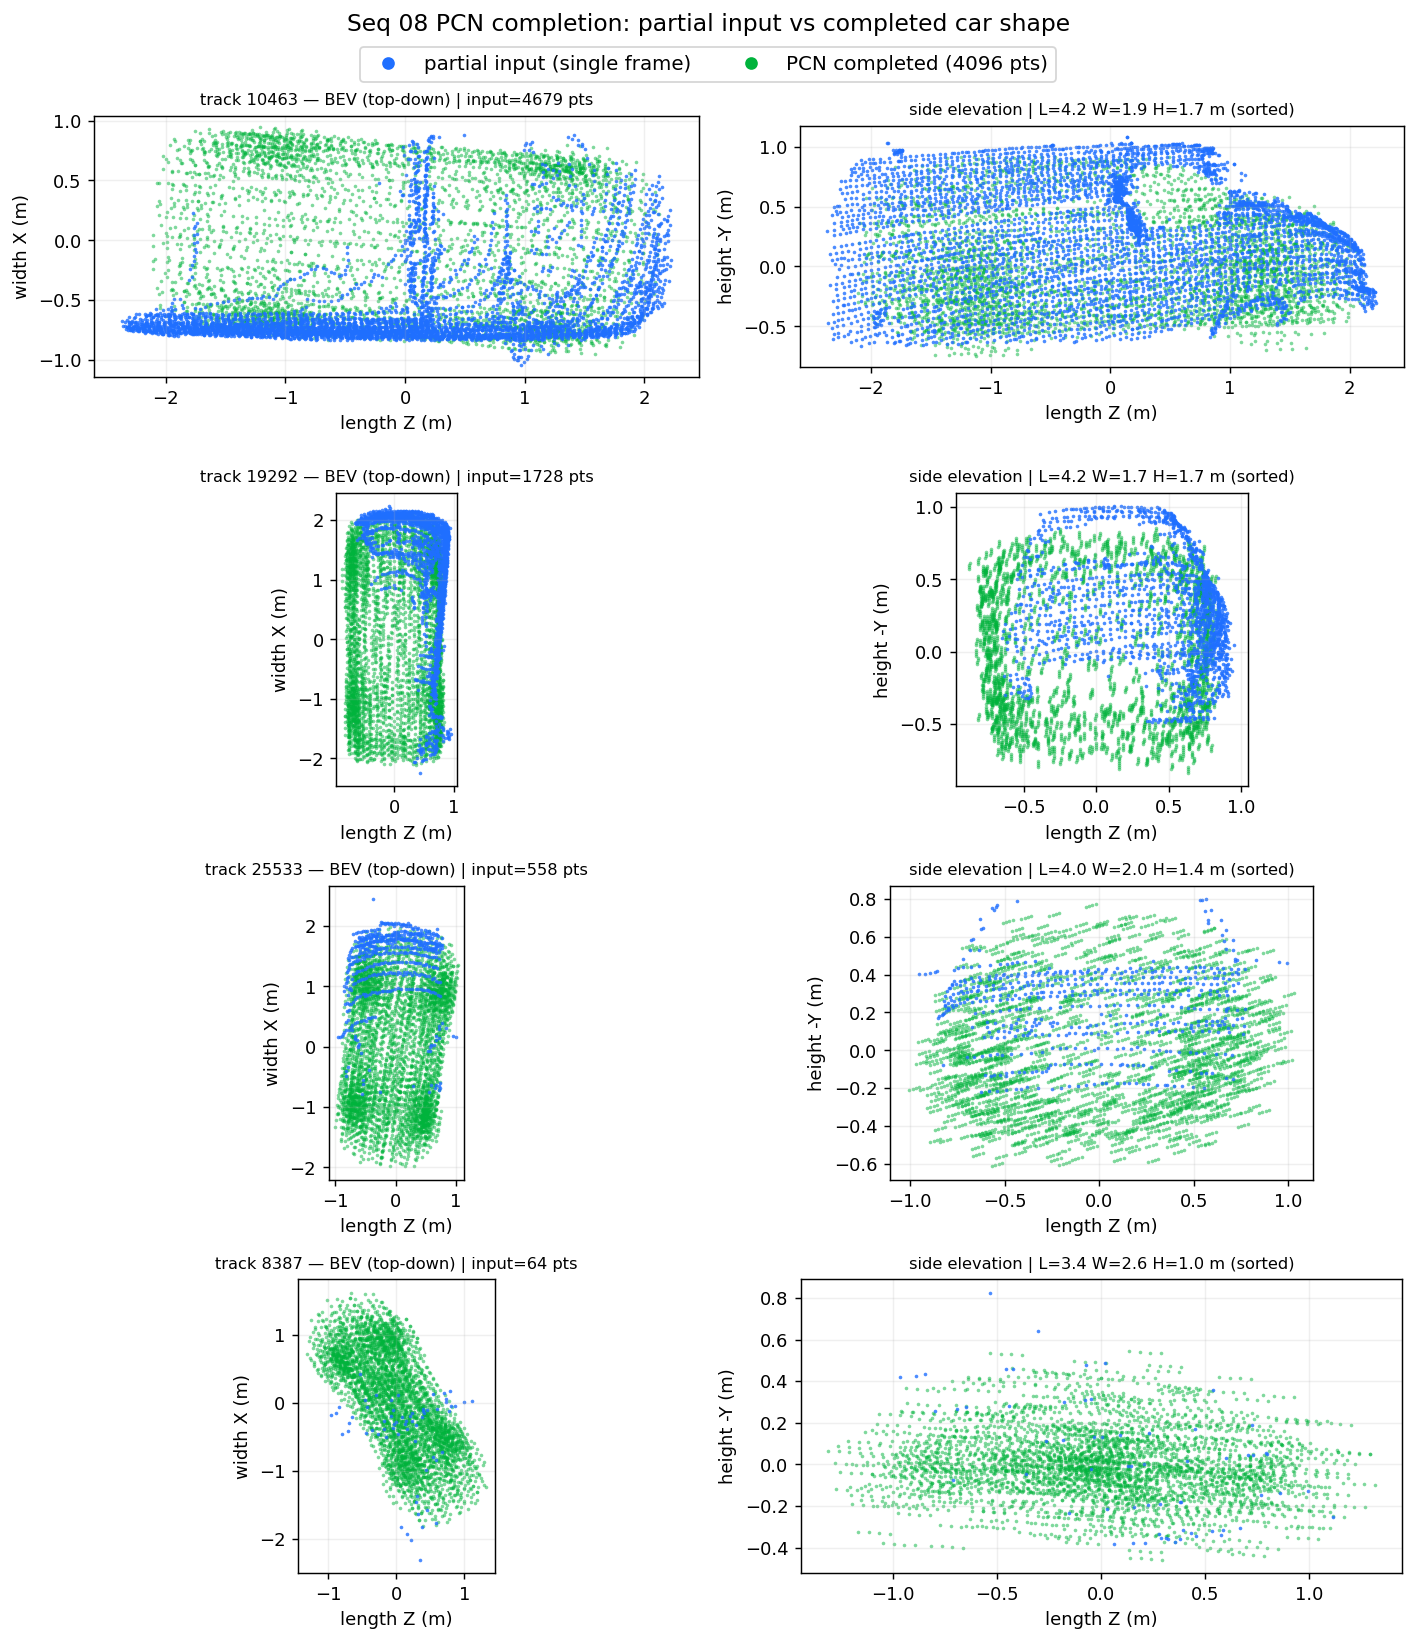
\includegraphics[width=0.92\textwidth]{completion_shape_08.png}
  \caption[Object completion on a real LiDAR car]{Object-level point-cloud completion on
    real sequence-08 cars. Each row is one detected car in bird's-eye (left) and side
    elevation (right): the blue points are the single-frame partial input the sensor
    observed from one side, and the green points are the PCN completion, which fills the
    occluded surface into a full car shape. This is the partial-to-complete mapping the
    thesis's completion stage performs; how well it does so on real data is evaluated in
    Section~\ref{sec:completion-results}.}
  \label{fig:completion-example}
\end{figure}

Two points from this literature bear directly on later chapters. First, models trained
on clean synthetic partials face a synthetic-to-real domain gap when applied to noisy,
sparse LiDAR clusters; this thesis adopts PCN and confronts that gap head-on
(Section~\ref{ch:completion-method}), and its comparison of PCN against a transformer alternative found no
decisive real-data advantage for the heavier model (Section~\ref{sec:completion-results}). Second, and more
consequentially, the standard completion metric, Chamfer distance to a reference
shape, presupposes a complete ground-truth surface, which real accumulated LiDAR does
not provide: the accumulation is itself one-sided, seen from the same road, so scoring a
completion against it rewards a network that reproduces the observed side and adds
nothing. This is why real-LiDAR completion is not evaluated by reference Chamfer at all
in the recent literature, and why this thesis evaluates it without any self-made
reference (Section~\ref{sec:completion-results}). This should be distinguished from
semantic scene completion, which fills a whole voxelised scene from a single scan;
the present work completes individual segmented objects, a different and narrower task.

Because real automotive LiDAR offers no complete target, a small toolkit of
completion metrics has grown up around the KITTI cars, of two kinds. The first kind is
reference-free fidelity: the unidirectional Chamfer and Hausdorff distances
(UCD and UHD), which score a completion by how closely it reproduces the points of its
own partial input. Chen et al.~\cite{chen2020unpaired} apply UHD directly to KITTI cars,
and P2C~\cite{cui2023p2c} uses UCD together with a region-aware variant (RCD) that
localises the comparison around observed skeleton points but still anchors it to seen
geometry. PCN~\cite{yuan2019pcnpointcompletionnetwork} scores its KITTI completions by
Fidelity (how well the input is preserved in the output), Minimal Matching
Distance (Chamfer distance to the nearest complete car in a synthetic reference set), and
Consistency (agreement between the completions of one instance across consecutive
frames); Ren et al.~\cite{ren2022selfsupervised} score completed vehicles against a
multi-frame accumulation with Chamfer-based distances. Every one of these references
something other than the real occluded surface, the observed input, a synthetic prior,
the model's own outputs, or a one-sided accumulation, and, crucially, a completion that
merely copies its input scores best on the input-referenced measures, so none of
them rewards recovering genuinely unobserved surface. The second kind exists precisely to
close that gap: a plausibility term that asks not how close a completion is to a
reference but whether it reads as a real object at all. Chen et
al.~\cite{chen2020unpaired} pair UHD with exactly such a term, the acceptance rate of a
shape classifier trained on external complete shapes (ModelNet40), chosen to avoid bias
toward the ShapeNet shapes the completion network was trained on. This thesis adopts that
plausibility protocol as its favorable real-data completion signal, and reports fidelity
alongside it with the caveat that fidelity rewards under-completion
(Section~\ref{sec:completion-results}).

Table~\ref{tab:completion-metrics} summarises this landscape against the two properties
the completion claim needs: whether a metric credits a completion for producing a
plausible whole object rather than reproducing its input, and what each scores a
completion against. The fidelity measures reward input reproduction; the plausibility
term is the one that credits a car-plausible completed shape.

\begin{table}[H]
  \centering
  \caption[Real-LiDAR completion metrics by type]{Established real-LiDAR completion
    metrics, by kind and by what each scores a completion against. The
    fidelity measures reward reproducing the observed input, so a completion that
    adds nothing scores best on them, and they cannot on their own credit a plausible
    completed shape. The plausibility term, an independent classifier's acceptance
    of the completed cloud, is the one that credits a car-plausible whole object; it is
    the protocol this thesis adopts as its favorable real-data signal
    (Section~\ref{sec:completion-results}).}
  \label{tab:completion-metrics}
  \small
  \renewcommand{\arraystretch}{1.2}
  \setlength{\tabcolsep}{6pt}
  \begin{tabular}{@{}p{2.6cm}p{2.4cm}p{4.4cm}c@{}}
    \toprule
    Metric & Kind & Scored against & Plausible shape \\
    \midrule
    UCD~\cite{cui2023p2c}       & fidelity & observed input & no \\
    UHD~\cite{chen2020unpaired} & fidelity & observed input & no \\
    Fidelity~\cite{yuan2019pcnpointcompletionnetwork} & fidelity & observed input & no \\
    MMD~\cite{yuan2019pcnpointcompletionnetwork} & reference & synthetic CAD prior & indirect \\
    Consistency~\cite{yuan2019pcnpointcompletionnetwork} & self-ref. & model's own frames (cross-frame) & no \\
    meanCD~\cite{ren2022selfsupervised} & reference & full multi-frame accumulation & no \\
    \midrule
    \textbf{Plausibility}~\cite{chen2020unpaired} & plausibility & external classifier's car-acceptance & yes \\
    \bottomrule
  \end{tabular}
\end{table}

\subsection{Positioning of This Work}
\label{sec:bg-positioning}

The pipeline studied here is a car-only instance detector built from training-free
clustering and a binary classifier, followed by object completion. It occupies a
different point in the design space from the benchmark leaders of
Section~\ref{sec:bg-deep}. Table~\ref{tab:positioning} sets that position out along the
axes on which it actually differs, approach, segmentation supervision, and output type
, rather than on an accuracy score. A shared accuracy column is deliberately omitted:
the published methods are scored by mIoU and panoptic quality across all classes, this
work by a car-only point-level F$_1$, and placing those figures in one column would invite
a comparison the metrics do not support. The accuracy gap is real, and is stated plainly
in the text below the table instead.

\begin{table}[H]
  \centering
  \caption[Positioning against representative SemanticKITTI methods]{Positioning
    against representative SemanticKITTI methods by approach, segmentation supervision,
    and output type, the axes on which this work actually differs. A reported-accuracy
    column is deliberately omitted: the published methods are scored by mIoU and panoptic
    quality across all classes and this work by a car-only point-level F$_1$, so no single
    accuracy column would be comparable across rows. The accuracy gap is stated in the
    text.}
  \label{tab:positioning}
  \small
  \renewcommand{\arraystretch}{1.25}
  \setlength{\tabcolsep}{5pt}
  \begin{tabular}{@{}p{2.7cm}p{3.7cm}p{3.5cm}p{3.0cm}@{}}
    \toprule
    Method & Approach & Supervision & Output \\
    \midrule
    RangeNet++~\cite{milioto2019rangenet++} & Range-image CNN, semantic & Dense per-point & Per-point class \\
    RandLA-Net~\cite{Hu_2020_CVPR} & Point-based, semantic & Dense per-point & Per-point class \\
    Cylinder3D~\cite{zhu2021cylindrical} & Voxel (cylindrical), semantic & Dense per-point & Per-point class \\
    \addlinespace[2pt]
    RangeNet++ \& PointPillars~\cite{behley2021panoptic} & Semantic net + detector, panoptic & Dense per-point + boxes & Per-point class + instance \\
    Panoptic-PolarNet~\cite{zhou2021panopticpolarnet} & End-to-end panoptic & Dense per-point + instance & Per-point class + instance \\
    DS-Net~\cite{hong2021dsnet} & End-to-end panoptic & Dense per-point + instance & Per-point class + instance \\
    EfficientLPS~\cite{sirohi2021efficientlps} & End-to-end panoptic & Dense per-point + instance & Per-point class + instance \\
    \midrule
    \textbf{This work} & Geometric clustering + binary classifier (+ completion) & None for segmentation; auto-mined weak labels for the classifier & Point-level car clusters (+ completion) \\
    \bottomrule
  \end{tabular}
\end{table}

Read as requirements, the table states the thesis's position plainly. On their own
benchmarks the supervised networks reach \numrange{52.2}{67.8} mIoU (semantic) and
\numrange{37.1}{57.4} PQ (panoptic) over the official test sequences~11--21, scored
across all classes; this work reports a car-only point-level F$_1$ of \num{0.812}
(recall \num{0.732} against the $\ge$-10-surviving-points denominator of
Chapter~\ref{ch:evaluation}, precision \num{0.911}) on sequence~08. These are not the
same measurement, none of the published metrics is this work's point-level car F$_1$,
and the published rows are all-class test-set scores while this work's is a car-only,
single-sequence one, so the lower accuracy is a difference of paradigm, not a lower
score on a shared axis, and this work does not contest the gap. What the pipeline offers
instead is a different set of properties: it
segments without any labelled point clouds, it runs on a single consumer GPU without a
training stage for detection (its runtime is reported in Section~\ref{sec:results-runtime}), and every stage of
its decision is inspectable, so its
failure modes can be, and are, root-caused rather than left opaque (the recall
shortfall is traced to clustering fragmentation, not classifier error, in Section~\ref{sec:recall-analysis}).
The accuracy gap is therefore a deliberate consequence of choosing interpretability and
zero additional manual annotation over benchmark accuracy, not an unexplained deficiency.

A related question the table anticipates is why the comparison is drawn against
segmentation methods rather than 3D object detection, the task the ``detector'' label
most naturally invokes. Detection benchmarks score oriented 3D bounding boxes by average
precision, as in PointPillars~\cite{lang2019pointpillars} and
CenterPoint~\cite{yin2021centerpoint}. This pipeline, however, emits point-level clusters
, it must, because those clusters are the input to the completion stage (Section~\ref{ch:completion-method}),
and never fits an oriented box; box AP would require a box-fitting stage the pipeline
deliberately does not have. Point-level IoU against the ground-truth car points is
therefore the metric that matches the actual output, and the choice of IoU threshold and
recall denominator that make that measurement precise, together with its sensitivity
to those choices, is examined directly in Section~\ref{sec:eval-protocol}.

This framing also sets the boundary of the thesis's contribution. The individual
building blocks, classical ground-removal-plus-clustering detection, including recent
clustering-plus-classifier detectors for LiDAR vehicles~\cite{lim2025longrange}; a
lightweight multi-object tracking stage used only to filter transient detections across
frames (in the tradition of 3D multi-object trackers such as
AB3DMOT~\cite{weng2020ab3dmot}, and not a contribution of this work); and PCN-style
completion, are all established, and are reimplemented and tuned here rather than
invented. The contribution is their integration: a modular, inspectable framework, requiring zero
additional manual annotation, that detects occluded vehicles and completes them on real
LiDAR, evaluated end to end, with its completion quality assessed by an independent
classifier so that no self-made reference is involved
(Section~\ref{sec:completion-results}). Two diagnostic findings sit alongside it: the
root-cause analysis of the recall bottleneck together with the chain of negative repair
results (Section~\ref{sec:recall-analysis}), and the finding that synthetic pretraining is
redundant for the classifier at scale (Chapter~\ref{ch:evaluation}). The positioning table
is the backdrop against which the contribution is argued: this is an interpretable system
built on auto-mined supervision, whose value is in what it explains and measures, not in
topping a benchmark it was never designed to win.

\section{Theoretical Background}
\label{sec:bg-theory}

This section fixes notation and states the standard definitions for the operators the
pipeline is built from, in the order a scan passes through them: ground-plane fitting, voxel
downsampling, density-based clustering, the point-set classifier, and the point-set
distances used for completion and its evaluation. Each is a textbook construction cited to
its source; the pipeline's own architectures and parameter choices are given in the method
chapters. A single LiDAR scan is written as a finite point set
$P = \{\mathbf{x}_i \in \mathbb{R}^3\}_{i=1}^{N}$.

\subsection{Ground-Plane Removal by RANSAC}
\label{sec:th-ransac}
A plane is a pair $(\mathbf{n}, d)$ with unit normal $\mathbf{n}\in\mathbb{R}^3$,
$\lVert\mathbf{n}\rVert = 1$, and offset $d$; a point lies on it when
$\mathbf{n}\cdot\mathbf{x} + d = 0$, and its signed distance to the plane is
\begin{equation}
  \delta(\mathbf{x};\mathbf{n},d) = \mathbf{n}\cdot\mathbf{x} + d .
\end{equation}
RANSAC~\cite{fischler1981random} fits the ground plane by repeatedly sampling three points,
forming the plane through them, and scoring it by its inlier set, the points closer than
a tolerance $\tau_g$,
\begin{equation}
  \mathcal{I}(\mathbf{n},d) = \bigl\{\, \mathbf{x}\in P : \lvert \delta(\mathbf{x};\mathbf{n},d)\rvert \le \tau_g \,\bigr\}.
\end{equation}
The candidate with the largest inlier set is kept and its inliers removed as ground. To draw
at least one all-inlier sample with probability $p$, given inlier fraction $w$ and $s=3$
points per sample, the required number of iterations is
\begin{equation}
  T = \left\lceil \frac{\log(1-p)}{\log\!\bigl(1 - w^{s}\bigr)} \right\rceil .
\end{equation}

\subsection{Voxel-Grid Downsampling}
\label{sec:th-voxel}
To reduce the range-dependent density bias before clustering, the non-ground points are
downsampled on a regular grid of side $v$. Each point maps to an integer cell index
\begin{equation}
  \mathrm{vox}(\mathbf{x}) = \left\lfloor \frac{\mathbf{x} - \mathbf{x}_{\min}}{v} \right\rfloor \in \mathbb{Z}^3
\end{equation}
(the floor taken per coordinate), where $\mathbf{x}_{\min}$ is the per-axis minimum corner
of the point set. Writing $P_c = \{\mathbf{x}\in P : \mathrm{vox}(\mathbf{x}) = c\}$ for the
points falling in cell $c$, every occupied cell is replaced by their centroid,
\begin{equation}
  \bar{\mathbf{x}}_c = \frac{1}{\lvert P_c\rvert} \sum_{\mathbf{x}\in P_c} \mathbf{x} .
\end{equation}

\subsection{Density-Based Clustering: DBSCAN and HDBSCAN}
\label{sec:th-clustering}
The non-ground points are grouped into objects by density. DBSCAN~\cite{ester1996dbscan}
uses a fixed radius $\varepsilon$ and a minimum count $m$: with the
$\varepsilon$-neighbourhood
$\mathcal{N}_\varepsilon(\mathbf{p}) = \{\mathbf{q}\in P : \lVert\mathbf{p}-\mathbf{q}\rVert \le \varepsilon\}$,
a point is a core point when
\begin{equation}
  \lvert \mathcal{N}_\varepsilon(\mathbf{p}) \rvert \ge m ,
\end{equation}
and clusters are the maximal sets connected through core points. A single $\varepsilon$
cannot serve both the dense near field and the sparse far field of a scan.
HDBSCAN~\cite{campello2013hdbscan,mcinnes2017hdbscan} removes the fixed radius. With the
core distance $d_{\mathrm{core}}(\mathbf{p})$ set to the distance from $\mathbf{p}$ to
its $m$-th nearest neighbour, it defines the mutual reachability distance
\begin{equation}
  d_{\mathrm{mreach}}(\mathbf{a},\mathbf{b}) = \max\!\bigl(\, d_{\mathrm{core}}(\mathbf{a}),\; d_{\mathrm{core}}(\mathbf{b}),\; \lVert\mathbf{a}-\mathbf{b}\rVert \,\bigr),
\end{equation}
builds a minimum spanning tree under it, and condenses the tree into a hierarchy indexed by
$\lambda = 1/d_{\mathrm{mreach}}$. A candidate cluster $C$ born at $\lambda_{\min}(C)$, losing
each point $\mathbf{p}$ at level $\lambda_{\mathbf{p}}$, has stability
\begin{equation}
  S(C) = \sum_{\mathbf{p}\in C} \bigl(\lambda_{\mathbf{p}} - \lambda_{\min}(C)\bigr),
\end{equation}
and the flat clustering is the set of disjoint clusters of maximum total stability.
Stability-based extraction is what lets one setting cluster both near and far cars; it is
also, as Section~\ref{sec:recall-analysis} shows, what splits a single car when an internal
density gap makes two sub-clusters individually more stable than the whole.

\subsection{Permutation-Invariant Point Classification}
\label{sec:th-pointnet}
The car/not-car classifier is built on PointNet~\cite{Qi_2017_CVPR}, whose defining property
is invariance to the ordering of its input points. A function of a point set is made
permutation-invariant by applying a shared map $h$ to each point, pooling with a symmetric
operator, and passing the pooled feature through a final map $g$:
\begin{equation}
  f(\{\mathbf{x}_1,\dots,\mathbf{x}_n\}) = g\!\left( \max_{i=1,\dots,n} h(\mathbf{x}_i) \right),
\end{equation}
the maximum taken coordinate-wise over the per-point feature vectors. Because the $\max$ pool
is symmetric, $f$ is independent of the order of the points; $h$ and $g$ are multilayer
perceptrons learned end-to-end. Chapter~\ref{ch:pipeline} applies this design to a single
cluster.

\subsection{Point-Set Distances and Completion-Quality Measures}
\label{sec:th-distances}
Completion and its evaluation are expressed through distances between point sets. The
Chamfer distance between sets $A$ and $B$ averages, in each direction, the squared
distance from every point to the nearest point of the other set,
\begin{equation}
  \mathrm{CD}(A,B) = \frac{1}{\lvert A\rvert}\sum_{\mathbf{a}\in A} \min_{\mathbf{b}\in B} \lVert\mathbf{a}-\mathbf{b}\rVert^2 \;+\; \frac{1}{\lvert B\rvert}\sum_{\mathbf{b}\in B} \min_{\mathbf{a}\in A} \lVert\mathbf{b}-\mathbf{a}\rVert^2 ,
\end{equation}
and is the standard training objective and synthetic-benchmark score for completion, where
a complete ground-truth shape $B$ exists~\cite{fan2017point,yuan2019pcnpointcompletionnetwork}.
On real LiDAR no such $B$ exists (Section~\ref{sec:bg-completion}), so completion is scored
by two reference-free measures instead. Detection is first scored by a point-level
intersection-over-union between a predicted cluster $Q$ and a ground-truth car's point set
$G$,
\begin{equation}
  \mathrm{IoU}(Q,G) = \frac{\lvert Q \cap G\rvert}{\lvert Q \cup G\rvert},
\end{equation}
a prediction matching a ground-truth object when $\mathrm{IoU}(Q,G)\ge 0.3$
(Chapter~\ref{ch:evaluation}).

For completion, unidirectional fidelity measures how well a completed cloud $C$
preserves the observed partial input $P$, by the directed distance from each observed
point to its nearest completed point. The unidirectional Chamfer distance
(UCD)~\cite{cui2023p2c} averages it and the unidirectional Hausdorff distance
(UHD)~\cite{chen2020unpaired} takes its worst case,
\begin{equation}
  \mathrm{UCD}(P,C) = \frac{1}{\lvert P\rvert}\sum_{\mathbf{p}\in P} \min_{\mathbf{c}\in C} \lVert\mathbf{p}-\mathbf{c}\rVert^2 ,
  \qquad
  \mathrm{UHD}(P,C) = \max_{\mathbf{p}\in P} \min_{\mathbf{c}\in C} \lVert\mathbf{p}-\mathbf{c}\rVert .
\end{equation}
Both are smallest when $C$ reproduces $P$ exactly, so they reward preserving the observed
side and cannot, alone, credit added surface, the caveat under which
Section~\ref{sec:completion-results} reports them. The second measure is
plausibility~\cite{chen2020unpaired}: an independent shape classifier
$\phi(\cdot)$, trained on external complete shapes and returning a probability per class,
judges whether a completed cloud reads as a car. Over a set of completions
$\{C_k\}_{k=1}^{K}$, the acceptance rate is the fraction the classifier assigns to the car
class,
\begin{equation}
  \mathrm{Acc} = \frac{1}{K}\sum_{k=1}^{K} \mathbf{1}\!\left[\, \arg\max_j \phi_j(C_k) = \mathrm{car} \,\right],
\end{equation}
reported together with the mean car-probability $\tfrac{1}{K}\sum_k \phi_{\mathrm{car}}(C_k)$.
Because $\phi$ is trained on shapes disjoint from the completion network's training set,
a high acceptance rate is evidence that completion produces genuinely car-plausible shapes
rather than shapes that merely resemble its own training data
(Section~\ref{sec:completion-results}).

Three points emerge from this review and set up the rest of the thesis. First, the accuracy
of mainstream LiDAR segmentation is inseparable from a dense per-point annotation budget,
which motivates the interpretable clustering-plus-classifier route taken here, built on
auto-mined supervision, and whose recall cost the later chapters measure and root-cause. Second, that
route's stage-level transparency is what makes such root-causing possible at all, where an
end-to-end network offers no stage to inspect. Third, completion on real LiDAR has no valid
reference-based score: every reference or fidelity metric is anchored to the observed input,
a synthetic prior, or a one-sided accumulation, and rewards a completion that reproduces its
input, so the field pairs them with a plausibility term that asks whether the completed
shape reads as a real object. These three points are the basis on which the thesis is built:
the interpretable framework the first two motivate, and the plausibility-based completion
evaluation the third calls for, are what its two research questions address
(Chapter~\ref{ch:introduction}). The chapter has also fixed the notation and standard
operators the later chapters build on. Chapter~\ref{ch:pipeline} turns those operators into
the detection pipeline and the completion method, in their configured, instantiated form.

% ===== END inlined ch2_background.tex =====
% ===== BEGIN inlined ch3_methodology.tex =====
% Chapter 3 -- Methodology (\input by main.tex): detection pipeline + object completion
% (completion half merged in below, formerly sec_6_completion_method.tex).
%
% Honesty-phrasing rules applied (personal_agenda P1):
%   - production classifier is the FROM-SCRATCH Stage B checkpoint
%     (stage_b_scratch_best.pth, Finding #31); synthetic Stage A pretraining
%     was DROPPED from the final pipeline and is kept only as Ch-4 ablation
%     material (#25/#30). We do NOT present two-stage training as a contribution.
%   - measured vs inferred evidence tiers marked in prose; timing numbers are
%     measured (timing_seq08_full_n4068.json), cited as such.
%   - every number traceable to a finding / output artifact.
%   - "the classifier's job is precision" claim deferred to the Ch-4 ablation.
%
\chapter{Proposed Methodology}
\label{ch:pipeline}

This chapter presents the proposed method: a modular detection-and-completion framework
for automotive LiDAR. Section~\ref{sec:meth-architecture} gives the overall architecture;
the sections that follow describe each stage in the order a scan flows through it, in its
configured, instantiated form. The general operators each stage is built from are defined
in Chapter~\ref{ch:background}; this chapter states how each is set up and connected here,
and the end-to-end evaluation is Chapter~\ref{ch:evaluation}.

\section{System Architecture}
\label{sec:meth-architecture}

The framework is a single system that turns a raw LiDAR scan into completed,
box-estimated cars. It is organised as two stages in sequence, each the subject of one
section below. The detection stage (Section~\ref{sec:meth-detection}) segments and
classifies car clusters from the raw scan, emitting an oriented bounding box and a stable
track identity per car. The completion stage (Section~\ref{ch:completion-method})
reconstructs each detected car's full surface from the one-sided partial a single frame
observes. Figure~\ref{fig:pipeline} shows the detection chain that produces every input the
completion stage consumes.

The design is deliberately modular and classical: classical geometry does the work
geometry solves well, and small learned models are used only where discrimination
needs them, so every stage is separately inspectable and its cost separately
measurable. This architecture is what lets the evaluation
(Chapter~\ref{ch:evaluation}) attribute the recall limit to a single stage rather than
to an opaque network.

\section{Detection Pipeline}
\label{sec:meth-detection}

This section describes the car-detection pipeline that produces every detection
evaluated in Chapter~\ref{ch:evaluation} and every cluster completed in
Section~\ref{ch:completion-method}. The
design is deliberately modular and classical: a chain of independent stages,
each with a small number of interpretable parameters, rather than an end-to-end
learned detector. This choice trades peak accuracy for interpretability,
reproducibility, and zero additional manual annotation, the classifier is trained on
labels mined automatically from existing semantic annotations
(Section~\ref{sec:pipeline-classifier}), and it is what lets Section~\ref{sec:recall-analysis}
root-cause the recall shortfall to a single stage rather than to an opaque
network.

The pipeline takes one raw LiDAR scan and emits a set of car detections, each an
oriented bounding box with a stable track identity across frames. Every stage
parameter lives in a single frozen configuration, fixed before the write-up began; the frozen
values are collected in Table~\ref{tab:pipeline-config}. Figure~\ref{fig:pipeline}
gives the full chain.

\subsection{Overview of the Modular Detection Pipeline}
\label{sec:pipeline-overview}

\begin{figure}[H]
  \centering
  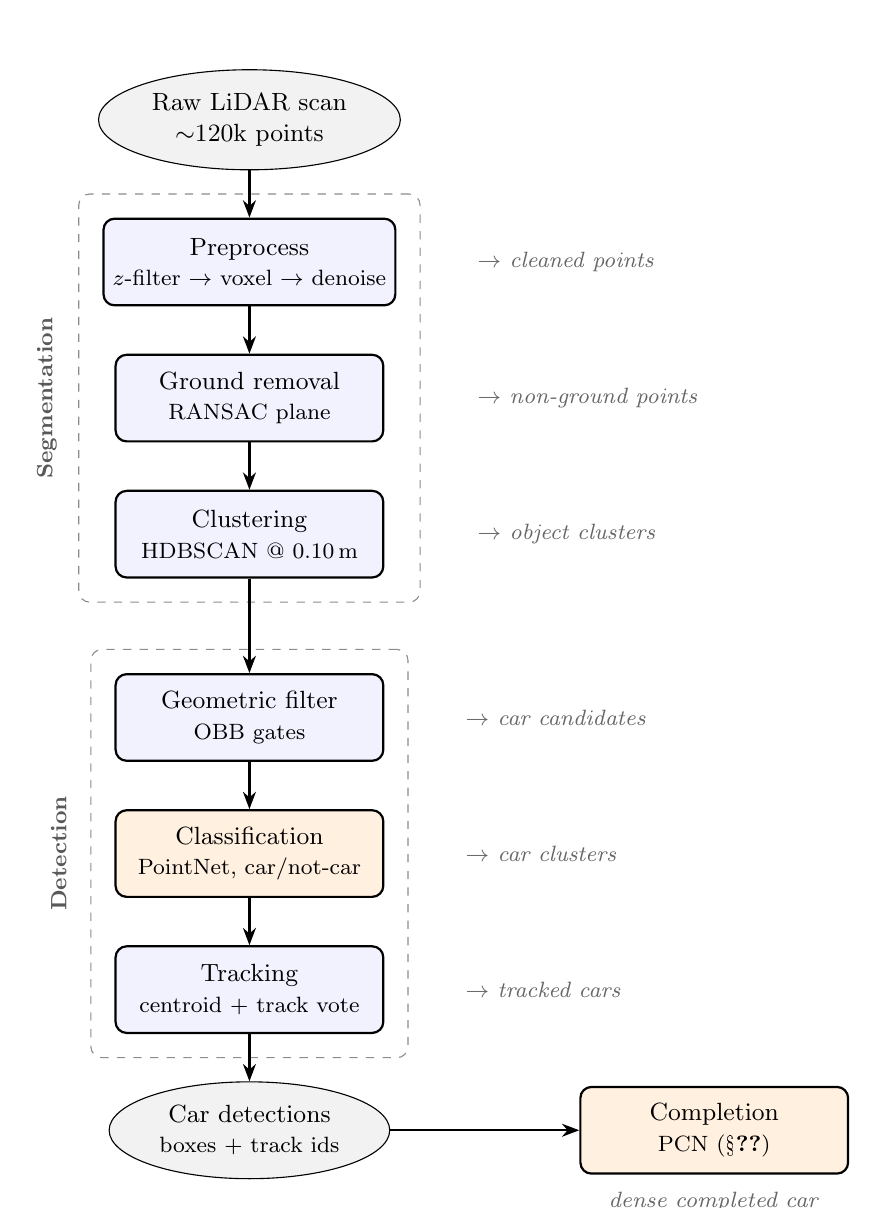
\begin{tikzpicture}[
      font=\small,
      node distance=6mm,
      stage/.style={
        draw, rounded corners, align=center,
        minimum width=34mm, minimum height=11mm,
        fill=blue!5, thick},
      learned/.style={stage, fill=orange!12},
      io/.style={draw, ellipse, align=center, fill=black!5,
        minimum width=28mm, minimum height=9mm},
      ms/.style={font=\footnotesize\itshape, text=black!60},
      arr/.style={-{Stealth[length=2.2mm]}, thick},
      grp/.style={draw=black!45, dashed, rounded corners, inner sep=3mm},
      grplab/.style={font=\footnotesize\bfseries, text=black!65},
    ]
    \node[io] (raw) {Raw LiDAR scan\\$\sim$120k points};
    \node[stage, below=of raw] (pre) {Preprocess\\{\footnotesize $z$-filter $\to$ voxel $\to$ denoise}};
    \node[stage, below=of pre] (ground) {Ground removal\\{\footnotesize RANSAC plane}};
    \node[stage, below=of ground] (cluster) {Clustering\\{\footnotesize HDBSCAN @ \SI{0.10}{\meter}}};
    \node[stage, below=12mm of cluster] (geo) {Geometric filter\\{\footnotesize OBB gates}};
    \node[learned, below=of geo] (clf) {Classification\\{\footnotesize PointNet, car/not-car}};
    \node[stage, below=of clf] (track) {Tracking\\{\footnotesize centroid + track vote}};
    \node[io, below=of track] (out) {Car detections\\{\footnotesize boxes + track ids}};
    \node[learned, right=24mm of out] (comp) {Completion\\{\footnotesize PCN (\S\ref{ch:completion-method})}};

    \draw[arr] (raw) -- (pre);
    \draw[arr] (pre) -- (ground);
    \draw[arr] (ground) -- (cluster);
    \draw[arr] (cluster) -- (geo);
    \draw[arr] (geo) -- (clf);
    \draw[arr] (clf) -- (track);
    \draw[arr] (track) -- (out);
    \draw[arr] (out) -- (comp);

    % dashed phase blocks (segmentation: points -> clusters; detection: clusters -> cars)
    \begin{scope}[on background layer]
      \node[grp, fit=(pre)(ground)(cluster)] (segbox) {};
      \node[grp, fit=(geo)(clf)(track)] (detbox) {};
    \end{scope}
    \node[grplab, rotate=90] at ([xshift=-4mm]segbox.west) {Segmentation};
    \node[grplab, rotate=90] at ([xshift=-4mm]detbox.west) {Detection};

    % per-stage output in one column, anchored to the phase-block right edge (uniform gap)
    \node[ms, anchor=west] at ([xshift=6mm]segbox.east|-pre)     {$\to$ cleaned points};
    \node[ms, anchor=west] at ([xshift=6mm]segbox.east|-ground)  {$\to$ non-ground points};
    \node[ms, anchor=west] at ([xshift=6mm]segbox.east|-cluster) {$\to$ object clusters};
    \node[ms, anchor=west] at ([xshift=6mm]detbox.east|-geo)     {$\to$ car candidates};
    \node[ms, anchor=west] at ([xshift=6mm]detbox.east|-clf)     {$\to$ car clusters};
    \node[ms, anchor=west] at ([xshift=6mm]detbox.east|-track)   {$\to$ tracked cars};
    \node[ms, below=1mm of comp.south, text width=34mm, align=center]
      {\footnotesize\itshape dense completed car};
  \end{tikzpicture}
  \caption[Detection pipeline]{The detection pipeline, grouped into two phases (dashed): a
    segmentation phase that turns a raw scan into clusters (preprocess, ground removal,
    clustering) and a detection phase that turns clusters into tracked car boxes
    (geometric filter, classification, tracking), with each stage's output shown at right; the
    completion stage (right) runs off the tracked detections. Learned stages are shaded; all
    others are classical.}
  \label{fig:pipeline}
\end{figure}

The system is offline by design: the tracker and the track-level filter
use the whole sequence, and real-time operation is out of scope. The pipeline runs well
below sensor rate, and the per-stage runtime budget, which stages dominate, and where
the learned and classical costs fall, is measured and reported in the runtime section
of Chapter~\ref{ch:evaluation} rather than claimed here.

\subsection{Preprocessing: Filtering, Downsampling, and Denoising}
\label{sec:pipeline-preprocess}

Each raw scan (roughly \num{120000} points) passes through three cleaning steps
before any object reasoning:

\begin{enumerate}
  \item Ground-height $z$-filter. Points below
    $z = \SI{-2.0}{\meter}$ in the sensor frame are dropped. This removes the bulk
    of the road surface and any sub-ground noise cheaply, before the more
    expensive steps see them.
  \item Voxel downsampling at \SI{0.05}{\meter}. Points are collapsed to
    one representative per \SI{5}{\centi\meter} voxel, which both regularises the
    range-dependent density of LiDAR and cuts the point count by roughly an order
    of magnitude.
  \item Statistical outlier removal. Points whose mean distance to their
    \num{20} nearest neighbours exceeds \num{2.0} standard deviations of the
    local distribution are discarded, removing isolated speckle.
\end{enumerate}

The order of the last two steps is behaviour-changing. In the frozen configuration
(\texttt{voxel\_\allowbreak before\_\allowbreak denoise = True}) downsampling runs before
denoising, so the statistical outlier test operates on roughly ten times fewer
points, and on a regularised point set, which changes which points survive.
This ordering was adopted as part of the pipeline optimisation primarily
because it improves detection (Chapter~\ref{ch:evaluation}). It is behaviour-changing, so
we flag it here rather than presenting the two orderings as equivalent.

\subsection{Ground-Plane Removal by RANSAC}
\label{sec:pipeline-ground}

The dominant remaining structure after preprocessing is the ground plane, which
must be removed before clustering or it bridges every object into one component.
We fit a single plane with RANSAC: over \num{300} iterations, three points are
sampled, their plane computed, and inliers counted within
\SI{0.2}{\meter}; the best-supported plane is kept. The plane is
accepted only if its normal is near-vertical, the $z$-component of the
unit normal must exceed \num{0.5}, so a spuriously-fitted vertical surface (a
wall, the side of a truck) cannot be mistaken for ground. If the check fails, no
points are removed and the whole cloud is passed on as objects; this fail-safe is
rare but prevents a bad plane fit from deleting real cars.

A single global plane is a deliberate simplification: it assumes the local ground
is approximately planar, which holds on the flat urban sequences used here but
would degrade on strong slopes. A grid-based ground model (Patchwork++-style) is
listed as future work, not a limitation we claim to have solved. The iteration
count was reduced from \num{1000} to \num{300} as part of the runtime optimisation after
confirming the plane fit converges well before \num{1000} iterations on this
data; the fit uses a fixed seed (\texttt{np.random.default\_rng(42)}) so ground
removal, and therefore the whole pipeline, is deterministic across runs.

\subsection{Object-Candidate Clustering with HDBSCAN}
\label{sec:pipeline-cluster}

Non-ground points are grouped into object candidates with HDBSCAN
(Section~\ref{sec:th-clustering} gives the general mutual-reachability construction), here
configured with a minimum cluster size of \num{10} and a minimum-samples value of \num{5}
(the neighbour count $m$ that sets the core distance). HDBSCAN is chosen over a fixed-radius method
because LiDAR density falls off with range: a single Euclidean radius that merges
nothing at \SI{5}{\meter} will over-segment at \SI{40}{\meter}. HDBSCAN's
variable-density hierarchy adapts to this without a hand-tuned radius schedule,
and Chapter~\ref{ch:evaluation} reports a controlled benchmark confirming it beats
DBSCAN and Euclidean extraction on recall at matched settings.

Two details of the frozen configuration are load-bearing. First, clustering runs
on a coarser \SI{0.10}{\meter} voxel grid than the \SI{0.05}{\meter}
preprocessing grid: the object cloud is re-downsampled to \SI{0.10}{\meter},
HDBSCAN is run there, and the labels are propagated back to the full-resolution
points by nearest neighbour. This was adopted because the coarser
grid closes intra-car density gaps that otherwise cause a single car to split
into several clusters, the central mechanism of the recall bottleneck analysed
in Section~\ref{sec:recall-analysis} (Figure~\ref{fig:clustering}); its measured effect on
true positives is reported there. Second, HDBSCAN is by far the pipeline's most expensive
stage, because it is superlinear in the point count, so the coarse-grid re-voxelisation is
as much a speed measure as an accuracy one; the per-stage runtime is reported in
Chapter~\ref{ch:evaluation}.

\begin{figure}[H]
  \centering
  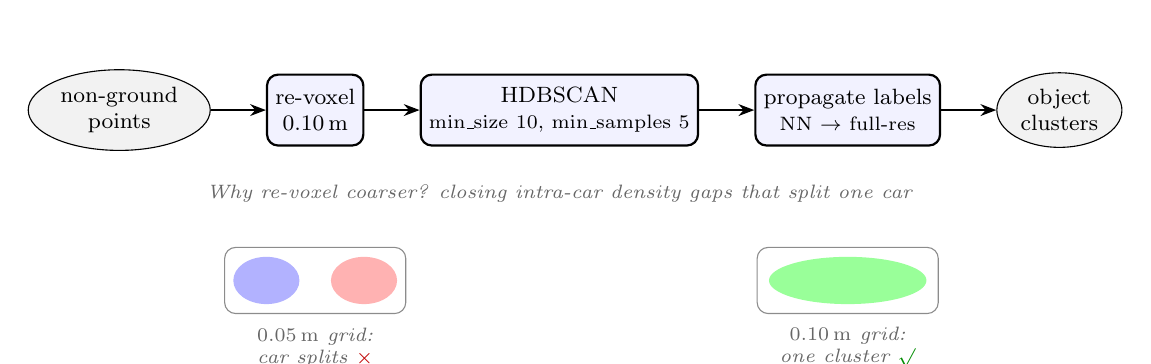
\begin{tikzpicture}[
      font=\footnotesize, node distance=5mm and 7mm,
      blk/.style={draw, rounded corners, align=center, fill=blue!5, thick,
        minimum height=9mm, inner sep=3pt},
      io/.style={draw, ellipse, align=center, fill=black!5, inner sep=2pt},
      arr/.style={-{Stealth[length=2mm]}, thick},
      note/.style={font=\scriptsize\itshape, text=black!60, align=center},
    ]
    % --- top: the clustering flow ---
    \node[io] (in) {non-ground\\points};
    \node[blk, right=of in] (vox) {re-voxel\\\SI{0.10}{\meter}};
    \node[blk, right=of vox] (hdb) {HDBSCAN\\{\scriptsize min\_size \num{10}, min\_samples \num{5}}};
    \node[blk, right=of hdb] (prop) {propagate labels\\{\scriptsize NN $\to$ full-res}};
    \node[io, right=of prop] (out) {object\\clusters};
    \draw[arr] (in)--(vox); \draw[arr] (vox)--(hdb);
    \draw[arr] (hdb)--(prop); \draw[arr] (prop)--(out);

    % --- bottom: why the coarser grid (split vs whole) ---
    \node[note] (why) at ($(hdb.south)+(0,-6mm)$)
      {Why re-voxel coarser? closing intra-car density gaps that split one car};
    \begin{scope}[shift={($(vox.south)+(0,-17mm)$)}]
      \draw[rounded corners, black!45] (-1.15,-0.42) rectangle (1.15,0.42);
      \fill[blue!30] (-0.62,0) ellipse (0.42 and 0.30);
      \fill[red!30]  (0.62,0)  ellipse (0.42 and 0.30);
      \node[note] at (0,-0.85) {\SI{0.05}{\meter} grid:\\car splits {\textcolor{red!75!black}{$\times$}}};
    \end{scope}
    \begin{scope}[shift={($(prop.south)+(0,-17mm)$)}]
      \draw[rounded corners, black!45] (-1.15,-0.42) rectangle (1.15,0.42);
      \fill[green!40] (0,0) ellipse (1.0 and 0.30);
      \node[note] at (0,-0.85) {\SI{0.10}{\meter} grid:\\one cluster {\textcolor{green!55!black}{$\surd$}}};
    \end{scope}
  \end{tikzpicture}
  \caption[Clustering stage]{The clustering stage. Non-ground points are re-voxelised to a coarser
    \SI{0.10}{\meter} grid, clustered with HDBSCAN (density-adaptive, so a single car stays whole at
    both near and far range without a hand-tuned radius), and the cluster labels are propagated back to
    the full-resolution points by nearest neighbour. The coarser grid is load-bearing (bottom): on the
    \SI{0.05}{\meter} preprocessing grid intra-car density gaps split one car into several clusters,
    whereas the \SI{0.10}{\meter} grid closes them and keeps the car a single cluster. HDBSCAN is the
    pipeline's most expensive stage, so the coarse grid is also a speed measure.}
  \label{fig:clustering}
\end{figure}

\subsection{Geometric Filtering of Non-Car Clusters}
\label{sec:pipeline-geometric}

Most clusters are not cars: they are trees, poles, building facades, and
fragments. A geometric filter rejects clusters whose oriented bounding box (OBB)
is inconsistent with a car, using only cheap, interpretable shape gates. For each
cluster the OBB is computed and the cluster is kept only if it passes all
of the following:

\begin{itemize}
  \item at least \num{15} points;
  \item OBB volume in $[\num{0.5}, \num{50}]\,\si{\meter\cubed}$;
  \item longest OBB extent $\leq \SI{6.0}{\meter}$, and the two largest extents
    above small floors (\SI{0.5}{} and \SI{0.4}{\meter}), rejecting slivers;
  \item box centre no more than \SI{1.5}{\meter} above the fitted ground plane,
    and vertical point span $\leq \SI{1.8}{\meter}$, rejecting tall structures;
  \item aspect ratio (longest\,/\,shortest extent) $\leq \num{6.0}$, rejecting
    thin walls and poles.
\end{itemize}

These bounds are generous car priors, not a tight car model, they are meant to
remove obvious non-cars while leaving the fine car/not-car decision to the
learned classifier. The height gate is computed relative to the fitted
ground plane, not to a fixed world height, so it is robust to the sensor not
being perfectly level. Its individual gates are ablated in Chapter~\ref{ch:evaluation}; the stage is
high-recall and low-precision by construction, and the
classifier is what turns its survivors into precise detections.

\subsection{The Car / Not-Car Point Classifier}
\label{sec:pipeline-classifier}

Each surviving cluster is classified as car or not-car by a small
dual-branch PointNet. The binary decision
replaces
an earlier multi-class (car/bus/motorcycle) design that was dropped once the data
showed near-zero real bus and motorcycle instances, leaving the car-only detector
(Chapter~\ref{ch:introduction}).

\paragraph{Architecture:} The network has two branches
(Figure~\ref{fig:classifier}) and about \num{80000}
parameters, deliberately small:
\begin{itemize}
  \item a point branch that takes \num{512} points (sampled or padded)
    normalised into the unit sphere, and applies shared per-point MLPs
    ($3 \to 64 \to 128 \to 256$) followed by a max-pool to a \num{256}-d shape
    descriptor;
  \item a bounding-box branch that takes an \num{8}-dimensional metric
    feature vector (sorted OBB extents, volume, two aspect ratios,
    $\log(1+\text{point count})$, vertical span), $z$-score normalised, through a
    small MLP to \num{32}-d.
\end{itemize}
The two are concatenated and passed through a small head
($288 \to 128 \to 2$) with dropout. The bounding-box branch is what re-injects
absolute metric scale, which the unit-sphere normalisation deliberately strips
from the point branch: a distant small car and a nearby one have the same
normalised shape but different real extents, and the metric branch is how the
network sees the difference. There are no T-Nets, since clusters already sit in a
consistent sensor frame.

\begin{figure}[H]
  \centering
  \resizebox{\linewidth}{!}{%
  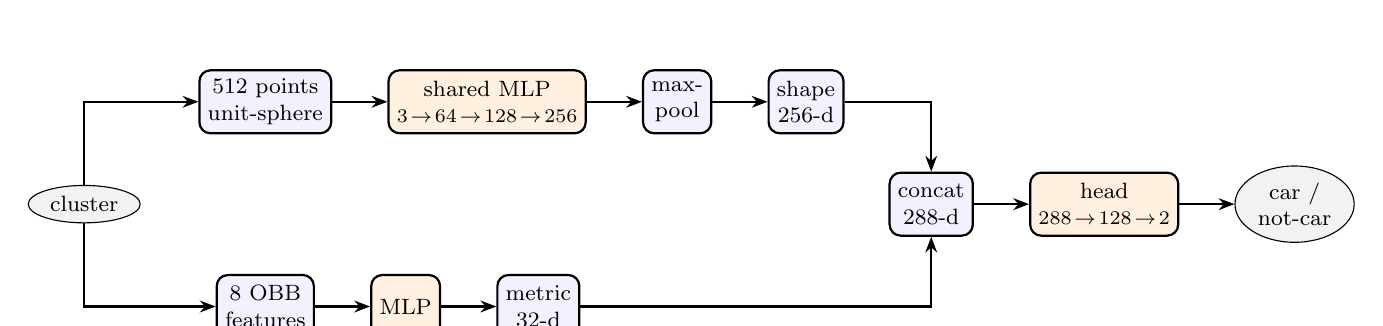
\begin{tikzpicture}[
      font=\footnotesize, node distance=6mm and 7mm,
      blk/.style={draw, rounded corners, align=center, fill=blue!5, thick,
        minimum height=8mm, inner sep=3pt},
      lrn/.style={blk, fill=orange!12},
      io/.style={draw, ellipse, align=center, fill=black!5, inner sep=2pt},
      arr/.style={-{Stealth[length=2mm]}, thick},
    ]
    \node[io] (cl) at (0,0) {cluster};
    \node[blk] (pts) at (2.3,1.3) {\num{512} points\\unit-sphere};
    \node[lrn, right=of pts] (pmlp) {shared MLP\\{\scriptsize $3\!\to\!64\!\to\!128\!\to\!256$}};
    \node[blk, right=of pmlp] (pool) {max-\\pool};
    \node[blk, right=of pool] (pd) {shape\\\num{256}-d};
    \node[blk] (feat) at (2.3,-1.3) {\num{8} OBB\\features};
    \node[lrn, right=of feat] (bmlp) {MLP};
    \node[blk, right=of bmlp] (bd) {metric\\\num{32}-d};
    \node[blk] (cat) at ($(pd.east)+(1.1,-1.3)$) {concat\\\num{288}-d};
    \node[lrn, right=of cat] (head) {head\\{\scriptsize $288\!\to\!128\!\to\!2$}};
    \node[io, right=of head] (out) {car /\\not-car};
    \draw[arr] (cl) |- (pts.west);
    \draw[arr] (cl) |- (feat.west);
    \draw[arr] (pts)--(pmlp); \draw[arr] (pmlp)--(pool); \draw[arr] (pool)--(pd);
    \draw[arr] (feat)--(bmlp); \draw[arr] (bmlp)--(bd);
    \draw[arr] (pd) -| (cat.north);
    \draw[arr] (bd) -| (cat.south);
    \draw[arr] (cat) -- (head);
    \draw[arr] (head) -- (out);
  \end{tikzpicture}%
  }
  \caption[Dual-branch classifier]{The dual-branch classifier applied to one
    cluster. The point branch takes \num{512} unit-sphere-normalised points to a
    \num{256}-d shape descriptor; the bounding-box branch takes \num{8} metric
    shape features to \num{32}-d. The two are concatenated and passed through a
    small head to a car/not-car decision. Learned blocks are shaded.}
  \label{fig:classifier}
\end{figure}

\paragraph{Training data (mined, not hand-labelled):} The classifier is trained
on real LiDAR clusters mined automatically from SemanticKITTI. For each training frame the pipeline's own
stages~1--5 are replayed, the ground-truth semantic labels are propagated onto the
surviving clusters by nearest neighbour, and each cluster is labelled car
or not-car by majority vote, keeping only clusters whose majority class
has purity $\geq \num{0.75}$. This yields \num{420333} training clusters
(sequences 00--07, 09, 10) and \num{130394} validation clusters (sequence~08),
with the intrinsic $\approx$21\,\%/79\,\% car/not-car imbalance handled by a
class-weighted loss. The key property is that the training clusters are produced
by the same clustering and filtering the classifier meets at inference,
including HDBSCAN splits and filter survivors, so it learns on exactly the
distribution it must classify, at no manual-annotation cost.

\paragraph{The from-scratch production checkpoint:} The production classifier
is \texttt{stage\_b\_\allowbreak scratch\_\allowbreak best.pth}, trained on the
mined real clusters from random initialisation. An earlier
two-stage design first pretrained on synthetic ShapeNet partial renders
(``Stage~A'') and then fine-tuned on the real clusters (``Stage~B''). The
two-stage machinery is reported in Chapter~\ref{ch:evaluation} as an ablation:
a controlled comparison there shows the synthetic pretraining to be redundant given the
mined real clusters, so the final pipeline uses the simpler from-scratch checkpoint, and
the synthetic pretraining, together with the finding that the sim-to-real gap is total and
symmetric, is presented as a negative result rather than as a contribution.

\paragraph{Training:} The from-scratch checkpoint is trained for \num{15} epochs
with Adam (learning rate \num{e-4}, weight decay \num{e-5}) and a step schedule
that halves the rate every \num{10} epochs, at batch size \num{64}. The loss is
cross-entropy weighted by inverse square-root class frequency (normalised to unit
mean), which offsets the intrinsic $\approx$21\,\%/79\,\% car/not-car imbalance
without resampling. Training clusters are augmented online with a random rotation
about the vertical axis and Gaussian jitter ($\sigma = \SI{0.005}{\meter}$); the
input is the \num{512}-point cluster of the architecture above. Runs are seeded
and the reported checkpoint is the epoch with the best validation macro-$F_1$; that
value, and the ablation comparison, are reported in Chapter~\ref{ch:evaluation}.

\subsection{Multi-Frame Tracking and Track-Level Filtering}
\label{sec:pipeline-tracker}

Detections are linked across frames by a centroid tracker. Each frame, current detections are matched to existing
tracks by solving a Hungarian assignment on the pairwise centroid-distance
matrix; matches beyond \SI{2.0}{\meter} are rejected, unmatched detections start
new tracks, and a track that goes unmatched for more than \num{5} consecutive
frames is retired. This is an offline, centroid-only tracker, no motion model,
no appearance, which is adequate here because detection, not association, is
the bottleneck; an IoU-based (SORT-style) tracker is listed as future work.

The tracker also enables a track-level filter that improves precision
(Figure~\ref{fig:tracker}).
Each detection carries the classifier's per-frame label; a track is accepted as a
car only if, across its lifetime, it collected at least \num{2} non-rejected
votes, those known votes are a majority of its votes
($\geq \num{0.5}$), and they agree on a single class. A cluster that the
classifier flickers on (a car in one frame, not-car in the next) is thus
resolved by temporal majority rather than trusted per frame. Because this filter
consults the whole track, it is an offline post-processing step, consistent with
the offline scope of the system; its contribution is isolated as an ablation row
in Chapter~\ref{ch:evaluation}. The tracker itself is computationally negligible.

\begin{figure}[H]
  \centering
  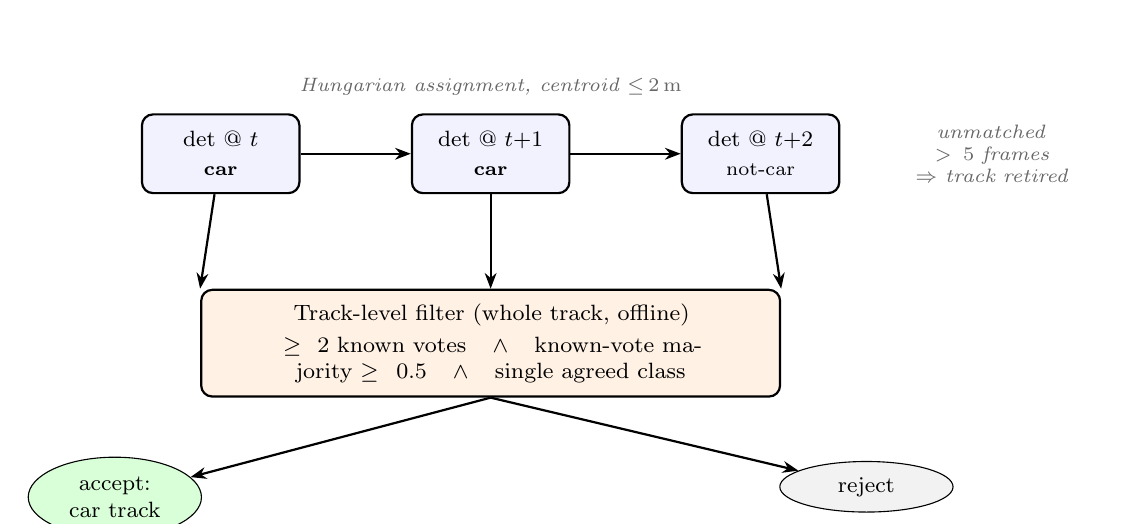
\begin{tikzpicture}[
      font=\footnotesize, node distance=6mm and 14mm,
      det/.style={draw, rounded corners, align=center, fill=blue!5, thick,
        minimum height=10mm, minimum width=20mm, inner sep=3pt},
      dec/.style={draw, rounded corners, align=center, fill=orange!10, thick, inner sep=5pt},
      res/.style={draw, ellipse, align=center, inner sep=3pt, minimum width=22mm},
      arr/.style={-{Stealth[length=2mm]}, thick},
      lbl/.style={font=\scriptsize\itshape, text=black!60, align=center},
    ]
    % one track's per-frame detections, linked by centroid association
    \node[det] (d1) {det @ $t$\\[1pt]{\scriptsize\bfseries car}};
    \node[det, right=of d1] (d2) {det @ $t{+}1$\\[1pt]{\scriptsize\bfseries car}};
    \node[det, right=of d2] (d3) {det @ $t{+}2$\\[1pt]{\scriptsize not-car}};
    \draw[arr] (d1)--(d2);
    \draw[arr] (d2)--(d3);
    \node[lbl, above=1mm of d2] {Hungarian assignment, centroid $\le$\,\SI{2}{\meter}};
    \node[lbl, right=6mm of d3, text width=24mm] (ret)
      {unmatched $>\num{5}$ frames\\$\Rightarrow$ track retired};

    % track-level filter over the whole vote sequence
    \node[dec, below=12mm of d2, text width=70mm] (filt)
      {Track-level filter (whole track, offline)\\[2pt]
       $\ge \num{2}$ known votes \;\, $\wedge$ \;\, known-vote majority $\ge \num{0.5}$
       \;\, $\wedge$ \;\, single agreed class};
    \draw[arr] (d1) -- (filt.north west);
    \draw[arr] (d2) -- (filt.north);
    \draw[arr] (d3) -- (filt.north east);

    \node[res, fill=green!15, below left=9mm and 3mm of filt] (acc) {accept:\\car track};
    \node[res, fill=black!5, below right=9mm and 3mm of filt] (rej) {reject};
    \draw[arr] (filt.south) -- (acc);
    \draw[arr] (filt.south) -- (rej);
  \end{tikzpicture}
  \caption[Tracker and track-level filter]{The tracker and track-level filter. Per-frame detections
    are linked into tracks by Hungarian assignment on centroid distance (matches beyond \SI{2}{\meter}
    rejected; a track unmatched for more than \num{5} frames retired). The track-level filter then
    resolves each track over its whole vote sequence rather than per frame: a track is accepted as
    a car only with at least \num{2} known votes, a known-vote majority of at least \num{0.5}, and
    agreement on a single class. In the worked example the votes \{car, car, not-car\} clear all three
    gates, so a classifier flicker in one frame is overruled by temporal majority. Both steps are
    offline.}
  \label{fig:tracker}
\end{figure}

\subsection{The Frozen Pipeline Configuration}
\label{sec:pipeline-config}

Table~\ref{tab:pipeline-config} lists the frozen parameter values that produce
every number in this thesis. They are the committed \texttt{PIPELINE\_CONFIG} and
were not altered to obtain any reported result.

\begin{table}[H]
  \centering
  \caption[Frozen pipeline configuration]{Frozen pipeline configuration. These values
    were fixed before the write-up; no reported number was produced by changing them.
    The classifier is the committed from-scratch checkpoint
    (\texttt{stage\_b\_scratch\_best.pth}).}
  \label{tab:pipeline-config}
  \begin{tabular}{lll}
    \toprule
    Stage & Parameter & Value \\
    \midrule
    Preprocess & $z$-filter threshold & \SI{-2.0}{\meter} \\
               & voxel size & \SI{0.05}{\meter} \\
               & denoise neighbours / std-ratio & \num{20} / \num{2.0} \\
               & voxel before denoise & true \\
    \midrule
    Ground     & RANSAC iterations & \num{300} \\
               & inlier distance & \SI{0.2}{\meter} \\
               & min.\ normal $z$ & \num{0.5} \\
    \midrule
    Clustering & method & HDBSCAN \\
               & min.\ cluster size / min.\ samples & \num{10} / \num{5} \\
               & clustering voxel size & \SI{0.10}{\meter} \\
    \midrule
    Geometric  & min.\ points & \num{15} \\
               & volume range & $[\num{0.5}, \num{50}]\,\si{\meter\cubed}$ \\
               & max.\ longest extent & \SI{6.0}{\meter} \\
               & max.\ height above ground & \SI{1.5}{\meter} \\
               & max.\ vertical span & \SI{1.8}{\meter} \\
               & max.\ aspect ratio & \num{6.0} \\
    \midrule
    Classifier & model & dual-branch PointNet (binary, from scratch) \\
               & input points & \num{512} \\
    \midrule
    Tracker    & max.\ match distance & \SI{2.0}{\meter} \\
               & max.\ disappeared frames & \num{5} \\
               & min.\ track length & \num{2} \\
               & min.\ known votes / ratio & \num{2} / \num{0.5} \\
    \bottomrule
  \end{tabular}
\end{table}

The completion stage that operates on the tracked car detections
(Figure~\ref{fig:pipeline}, right) is the subject of Section~\ref{ch:completion-method}; the evaluation of
the detections themselves is Chapter~\ref{ch:evaluation}.


%% ===== merged from sec_6_completion_method.tex ===== %%

% Point-Cloud Completion: Method (clean-method-first; false starts gathered in a
% closing "Negative results and lessons" subsection). Folds under Chapter 3.
%
% Scope: this section is the completion METHOD and the debugging narrative that
% produced it. The completion RESULTS (synthetic CD/F, independent-classifier
% plausibility, fidelity) live in Chapter 4 (Evaluation); here we only describe the
% method and defer the full evaluation.
%
% Reframe (2026-09-12): the old self-made completion metric and box-reference
% evaluation are dropped; result numbers migrated to Ch4 per the Ch3=theory rule.
%
% Honesty-phrasing rules applied (personal_agenda P1):
%   - domain-gap failures (#15-19) presented as FINDINGS, not apologies; #26
%     inference bug presented as a debugging lesson.
%   - final path = per-car length estimate ON.
%   - length-prior fallback stated as a live limitation.
%   - measured vs inferred tiers marked; numbers traceable to findings/artifacts.
%
% Figures (all embedded via \graphicspath from the gitignored output/ tree;
% regenerable from the named scripts):
%   Fig 6.1 fig61_partial_compare.py    -> fig61_partials/       (naive vs KITTI-like partial)
%   Fig 6.3 viz_completion.py           -> completion_shape_08.png (final output, output/08)
% Floats set [htbp]. Draft-grade renders; may get a cosmetic restyle in the figure pass.
%
\section{Object Completion}
\label{ch:completion-method}

This part of the method takes each detected car and completes it:
from the one-sided, partial cluster a single LiDAR frame observes, it predicts
the full car surface. The section presents the finished method in the order a
cluster passes through it, the network, its training data, the inference-time
normalisation, the input gate, and the length geometry, and then, separately,
gathers the negative results and lessons that shaped it
(Section~\ref{sec:completion-lessons}). Those false starts are of independent value
, one is the motivating case for a project-wide rule, so they are reported as
findings rather than smoothed over, but they are kept out of the method description
so that reads as what the pipeline does, not as how it was arrived at. The engineering
content here is not the network, a standard Point Completion Network (PCN) used off the
shelf, but the data it is trained on and the geometry by which a real partial is
presented to it. The evaluation of the finished method, on synthetic shapes and on real
cars by independent-classifier plausibility, is the subject of
Section~\ref{sec:completion-results}; here we describe how the completion is produced.

\subsection{Completion Targets: Single-Frame Car Clusters}
\label{sec:completion-what}

Completion runs on the tracked car detections of Section~\ref{sec:meth-detection}. The input is a
single-frame cluster in the sensor frame, not the accumulated multi-frame
track. This is a deliberate choice with an evidence basis: accumulating a moving car over many frames produces a
motion smear up to several metres long, which is neither a valid completion
target nor matchable to a car shape. A single frame is one clean, if partial,
observation. Whether completing this partial produces a car-plausible shape on real data
is what Section~\ref{sec:completion-results} measures; this section is how the completion
is produced.

\subsection{The Completion Network (PCN)}
\label{sec:completion-pcn}

We use PCN (Yuan et al., 2018), an encoder--decoder for point clouds
(Figure~\ref{fig:pcn}). The encoder is a stacked PointNet: shared per-point MLPs
lift each point to a local feature, a max-pool summarises the whole cloud into a
global vector, that global vector is concatenated back onto every point, and a
second MLP-plus-max-pool stage produces a single \num{1024}-dimensional shape
embedding. The decoder is coarse-to-fine: a fully-connected stage predicts
\num{1024} coarse seed points, then a grid-folding stage attaches a small
2D grid patch to each seed and learns to fold it into local surface geometry,
densifying the coarse skeleton into the final cloud. Training minimises a
two-term Chamfer loss, $\mathrm{CD}_{\text{coarse}} + 0.5\,\mathrm{CD}_{\text{fine}}$;
the fine term is down-weighted so the coarse skeleton is learned first. At
inference the partial is subsampled to \num{256} points before it enters the
encoder.

\begin{figure}[H]
  \centering
  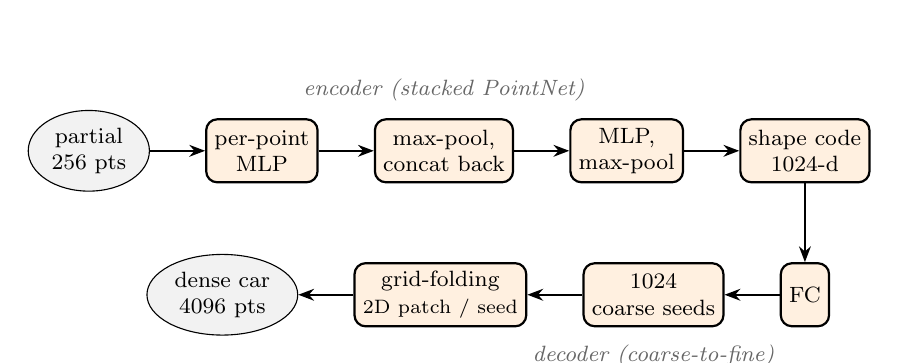
\begin{tikzpicture}[
      font=\footnotesize, node distance=6mm and 7mm,
      blk/.style={draw, rounded corners, align=center, fill=orange!12, thick,
        minimum height=8mm, inner sep=3pt},
      io/.style={draw, ellipse, align=center, fill=black!5, inner sep=2pt},
      arr/.style={-{Stealth[length=2mm]}, thick},
      lbl/.style={font=\footnotesize\itshape, text=black!60},
    ]
    \node[io] (in) {partial\\\num{256} pts};
    \node[blk, right=of in] (ppm) {per-point\\MLP};
    \node[blk, right=of ppm] (mp1) {max-pool,\\concat back};
    \node[blk, right=of mp1] (mp2) {MLP,\\max-pool};
    \node[blk, right=of mp2] (emb) {shape code\\\num{1024}-d};
    \node[blk, below=10mm of emb] (fc) {FC};
    \node[blk, left=of fc] (coarse) {\num{1024}\\coarse seeds};
    \node[blk, left=of coarse] (fold) {grid-folding\\{\scriptsize 2D patch / seed}};
    \node[io, left=of fold] (out) {dense car\\\num{4096} pts};
    \draw[arr] (in)--(ppm); \draw[arr] (ppm)--(mp1); \draw[arr] (mp1)--(mp2);
    \draw[arr] (mp2)--(emb); \draw[arr] (emb)--(fc); \draw[arr] (fc)--(coarse);
    \draw[arr] (coarse)--(fold); \draw[arr] (fold)--(out);
    \node[lbl, above=1mm of mp1] {encoder (stacked PointNet)};
    \node[lbl, below=1mm of coarse] {decoder (coarse-to-fine)};
  \end{tikzpicture}
  \caption[Completion network (PCN)]{The completion network (PCN). A stacked-PointNet
    encoder maps the \num{256}-point partial to a \num{1024}-d global shape code;
    a coarse-to-fine decoder predicts \num{1024} seed points and folds a small 2D
    grid patch onto each to produce the dense \num{4096}-point car. Every block is
    learned; the architecture is used off the shelf and unmodified.}
  \label{fig:pcn}
\end{figure}

The architecture is not a contribution and was not modified; the controlled comparison
against PoinTr that justifies keeping PCN, a small synthetic edge and equivalent
real-data behaviour, is reported with the completion ablations
(Section~\ref{sec:abl-completion}). What makes PCN
work on real cars is not the weights but the two subsections that follow: the
distribution of partials it is trained on, and the frame a real partial is normalised
into at inference.

\subsection{Training Data: KITTI-Like Partials}
\label{sec:completion-kittilike}

PCN is trained on synthetic partials, and those partials must match the distribution
of the real clusters it meets at inference or the network sees a different input at
test time than it was trained on. A derisk study comparing candidate partial
generators against real seq-08 clusters isolated three properties a naive
generator gets wrong: it sampled a dense pinhole depth render, skipped the
\SI{0.05}{\meter} voxelisation and ground removal the real input has been through, and
added range-proportional noise (up to \SI{0.15}{\meter} at \SI{30}{\meter}) that
washed out the scan-ring banding real Velodyne data shows.

The generator used makes the synthetic partial match the real one: it orients the
ShapeNet car to gravity, casts a single HDL-64E viewpoint (64 elevation beams,
\SI{0.09}{\degree} horizontal resolution) from a sensor at \SI{1.73}{\meter} and
a sampled range of \SIrange{8}{30}{\meter}, adds small absolute noise
(\SI{0.015}{\meter}), voxelises at \SI{0.05}{\meter} to match the pipeline, and
removes points within \SI{0.30}{\meter} of the ground plane. The dense complete
mesh sample remains the target. PCN retrained on these partials
(\texttt{pcn\_kitti\_best.pth}) is in-distribution with the real input, and on a held-out
synthetic set produces clean cars rather than blobs; its synthetic Chamfer and F-score are
reported in Chapter~\ref{ch:evaluation}. Figure~\ref{fig:kitti-like-partial} contrasts the
naive and KITTI-like partials for the same ShapeNet car.

\paragraph{Training:} PCN is trained on the KITTI-like synthetic partials (input
\num{256} points, target the dense mesh sample) for \num{100} epochs with Adam
(learning rate \num{e-4}, weight decay \num{e-6}) and a step schedule that halves
the rate every \num{40} epochs, at batch size \num{8}, minimising the two-term
Chamfer loss above. No real cars enter training; the reported checkpoint
(\texttt{pcn\_kitti\_best.pth}) is the best-validation-loss epoch. The subsequent geometry
work is all inference-time and does not retrain the network.

\begin{figure}[htbp]
  \centering
  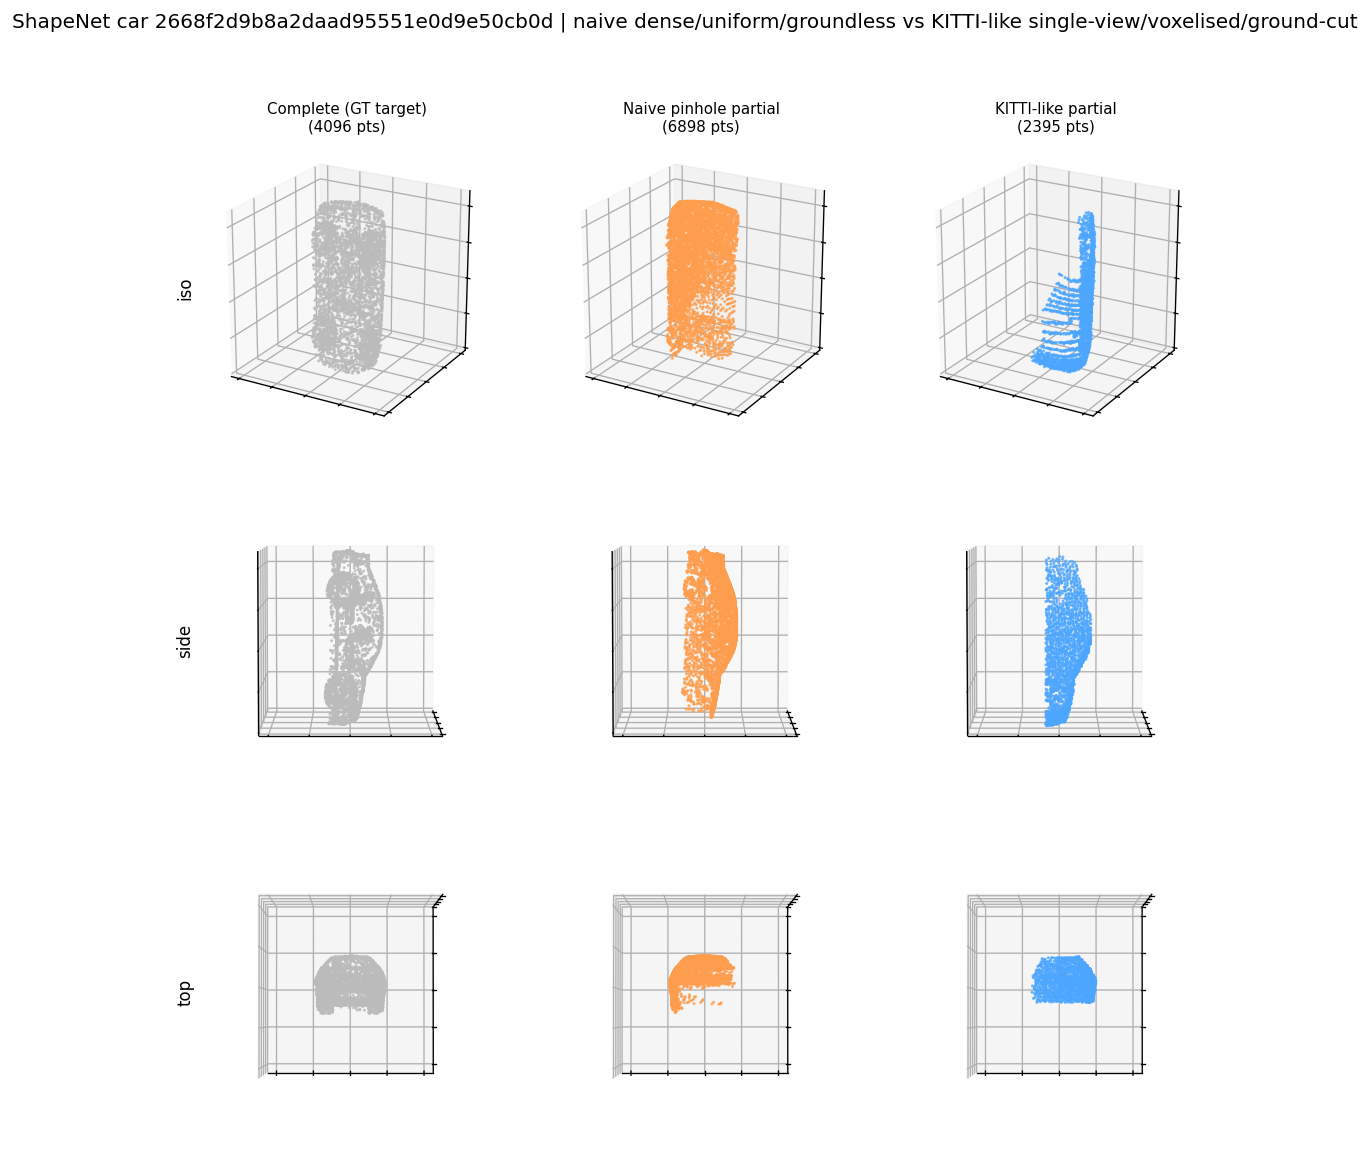
\includegraphics[width=\linewidth]{fig61_partials/partials_2668f2d9b8a2daad95551e0d9e50cb0d.png}
  \caption[Training-input distribution]{The training-input distribution: one ShapeNet car in
    three views, with its complete-surface target (left, grey) and two candidate
    training inputs. The naive pinhole partial (centre, orange) is dense and
    uniform; the KITTI-like partial (right, blue) reproduces what real LiDAR
    delivers, scan-ring banding, single-viewpoint coverage, \SI{0.05}{\meter}
    voxelisation, and the ground cut. Neither is a completion output; ``better''
    here means closer to the real input distribution, not more complete. Training on
    the KITTI-like distribution is what keeps the network in-distribution on real data.}
  \label{fig:kitti-like-partial}
\end{figure}

\subsection{Inference-Time Partial Normalisation}
\label{sec:completion-normalisation}

PCN is trained on shapes expressed in a fixed canonical car frame, centred on the
true car centre and scaled by the true car radius, so at inference a real partial
must be mapped into that same frame before it is completed, anything else
hands the network a normalisation it never saw during training. Reconstructing that
frame from a one-sided partial is non-trivial, because a partial reveals neither the
true centre nor the true radius directly. The inference path
(\texttt{estimate\_canonical\_frame}) reconstructs it in three steps:

\begin{itemize}
  \item Reorientation. The sensor frame is rotated into the canonical
    car frame (X${}={}$width, Y${}={}$up, Z${}={}$length): gravity maps to the
    up axis, and the horizontal heading axis maps to length. Heading comes from the
    L-shape footprint fit (Section~\ref{sec:completion-lshape}), not a principal-axis
    alignment.
  \item Full-car centre estimate. A one-sided partial's bounding-box
    centre is not the car centre, so the centre is corrected on each axis: shift
    down to undo the upward bias from the ground cut (the dominant
    correction, \SI{0.25}{\meter}); push outward along width toward the
    occluded far side to a half-car-width prior (\SI{1.9}{\meter}); and push
    along length toward the occluded far end (Section~\ref{sec:completion-length}).
  \item Scale. Normalise by the maximum point-to-centre distance divided
    by a fixed scale correction (\num{1.137}), the calibrated ratio between a
    one-sided partial radius and the true car radius.
\end{itemize}

With this path the same real seq-08 clusters recover the correct pose and scale; the
ablation isolating this normalisation against a naive partial-frame alternative, and the
box-overlap gains it produces, is reported with the completion ablations
(Section~\ref{sec:abl-completion}). Viewed in the
canonical car frame, the corrected completions are recognisably car-shaped: they
recover the car footprint in bird's-eye view and a rough side silhouette
(roofline included) even from very sparse input, a clean car footprint from a
\num{64}-point cluster in the extreme case. We are nonetheless careful about the
strength of the claim: crispness varies with input density (cleaner on
well-observed cars, blobbier on the sparsest), and a completion is a filled
\num{4096}-point cloud rather than a CAD-clean surface. The sharpest completions
are the in-distribution synthetic ones of
Section~\ref{sec:completion-kittilike}; on real data the normalisation's value is
corrected geometry, pose and scale, and the car-plausibility of the completed shape
that Section~\ref{sec:completion-results} reports. A calibration study on synthetic cars
further identified the residual dominant error as centre estimation, not scale,
which is what motivates the geometry work in the rest of this section.

\subsection{L-Shape Gating of Completion Inputs}
\label{sec:completion-lshape}

Even with correct normalisation, some clusters cannot complete into a plausible
car because the input is not one car: HDBSCAN fragments (part of a car) and
merges (two cars, or a \SI{90}{\degree} heading error) both feed the completion
network implausible input. To detect them we fit the cluster's ground-plane footprint with a
search-based L-shape fit (Zhang et al., 2017), which scores edge adherence over
candidate yaw angles and stays well-defined on near-square footprints where PCA
degenerates. The fitted footprint gives an input-quality gate: a
cluster is rejected as a fragment if its fitted length is below \SI{2.7}{\meter},
or as a merge if its fitted width exceeds \SI{2.3}{\meter}.

On seq-08 every implausible completion
originated from a fragment or merge input, so the gate's effect on completion quality
is a clean ablation, reported in Section~\ref{sec:abl-completion}. An honest secondary
finding from the same study: the L-shape heading itself is neutral against plain PCA on
real data, the fit earns its place by detecting bad inputs, not by giving a
better heading.

\subsection{Per-Car Length Estimation}
\label{sec:completion-length}

The canonical-frame centre estimate re-centres the occluded lateral side and the
ground cut, but a partial truncated at the occluded far end is normalised
around its observed near portion, so PCN's output tends to stop short of the far end,
the least-covered region of a one-sided car. Two successive fixes address it, both
inference-only (no retraining).

\paragraph{The fixed length prior:} A longitudinal, extend-only
push mirrors the width prior along the length axis: the centre is pushed toward
the occluded far end so the completion reaches an assumed full car length of
\SI{4.14}{\meter}, a population-median car length. A larger \SI{4.5}{\meter} prior
was rejected because it over-extended genuinely compact cars.

\paragraph{The per-car estimate:} A single \SI{4.14}{\meter}
prior is a population median, so it is wrong in both tails, it over-extends
compact cars and under-extends long ones. It is replaced by a per-car length,
\texttt{track\_length\_estimate}: the \nth{90} percentile of the car's own
gate-passed footprint-length fits, plus a \SI{0.12}{\meter} bias correction,
falling back to the fixed prior when a track has fewer than \num{5} gate-passed
frames. The aggregate is a quantile, not the maximum, because a single
contaminated L-shape fit would set the maximum. This is a per-track quantity, so the
pipeline (which owns the track) computes it and passes it in; the completion module itself
stays stateless.

\paragraph{Limitation:} The fallback is not rare: a non-trivial fraction of tracks have
fewer than five gate-passed frames and fall back to the fixed prior. This is stated as a
live limitation, not a solved problem; the exact fallback rate on sequence~08 is reported
with the completion results, and it is revisited in the discussion.

\subsection{The End-to-End Completion Path}
\label{sec:completion-summary}

To summarise, a single-frame car cluster is completed by: fitting its footprint
and rejecting fragments and merges (L-shape gate); reorienting it into the
canonical car frame with no PCA; estimating the full-car centre (down-shift for
the ground cut, width prior for the occluded side, per-car length estimate for
the occluded far end); normalising by the scale-corrected radius; running the
KITTI-like-trained PCN; and rotating the output back to the sensor frame. Every
step is inference-time geometry except the one-off retraining on KITTI-like
partials; no step fine-tunes on the evaluation cars.

Figure~\ref{fig:completion-shape} shows what this path produces on real seq-08
cars across the input-density range, in the canonical car frame. The completed
cloud (green) fills the car footprint and a rough side silhouette that the
single-frame partial (blue) leaves one-sided, recognisably car-shaped down to a
\num{64}-point input. Consistent with the caveats above, the sparsest inputs complete
more coarsely and can inflate the width, and the clouds are filled rather than CAD-clean;
the point here is qualitative shape, with the quantitative real-data assessment,
whether the completed cloud reads as a car to an independent classifier, being what
Section~\ref{sec:completion-results} sets out to measure.

\begin{figure}[htbp]
  \centering
  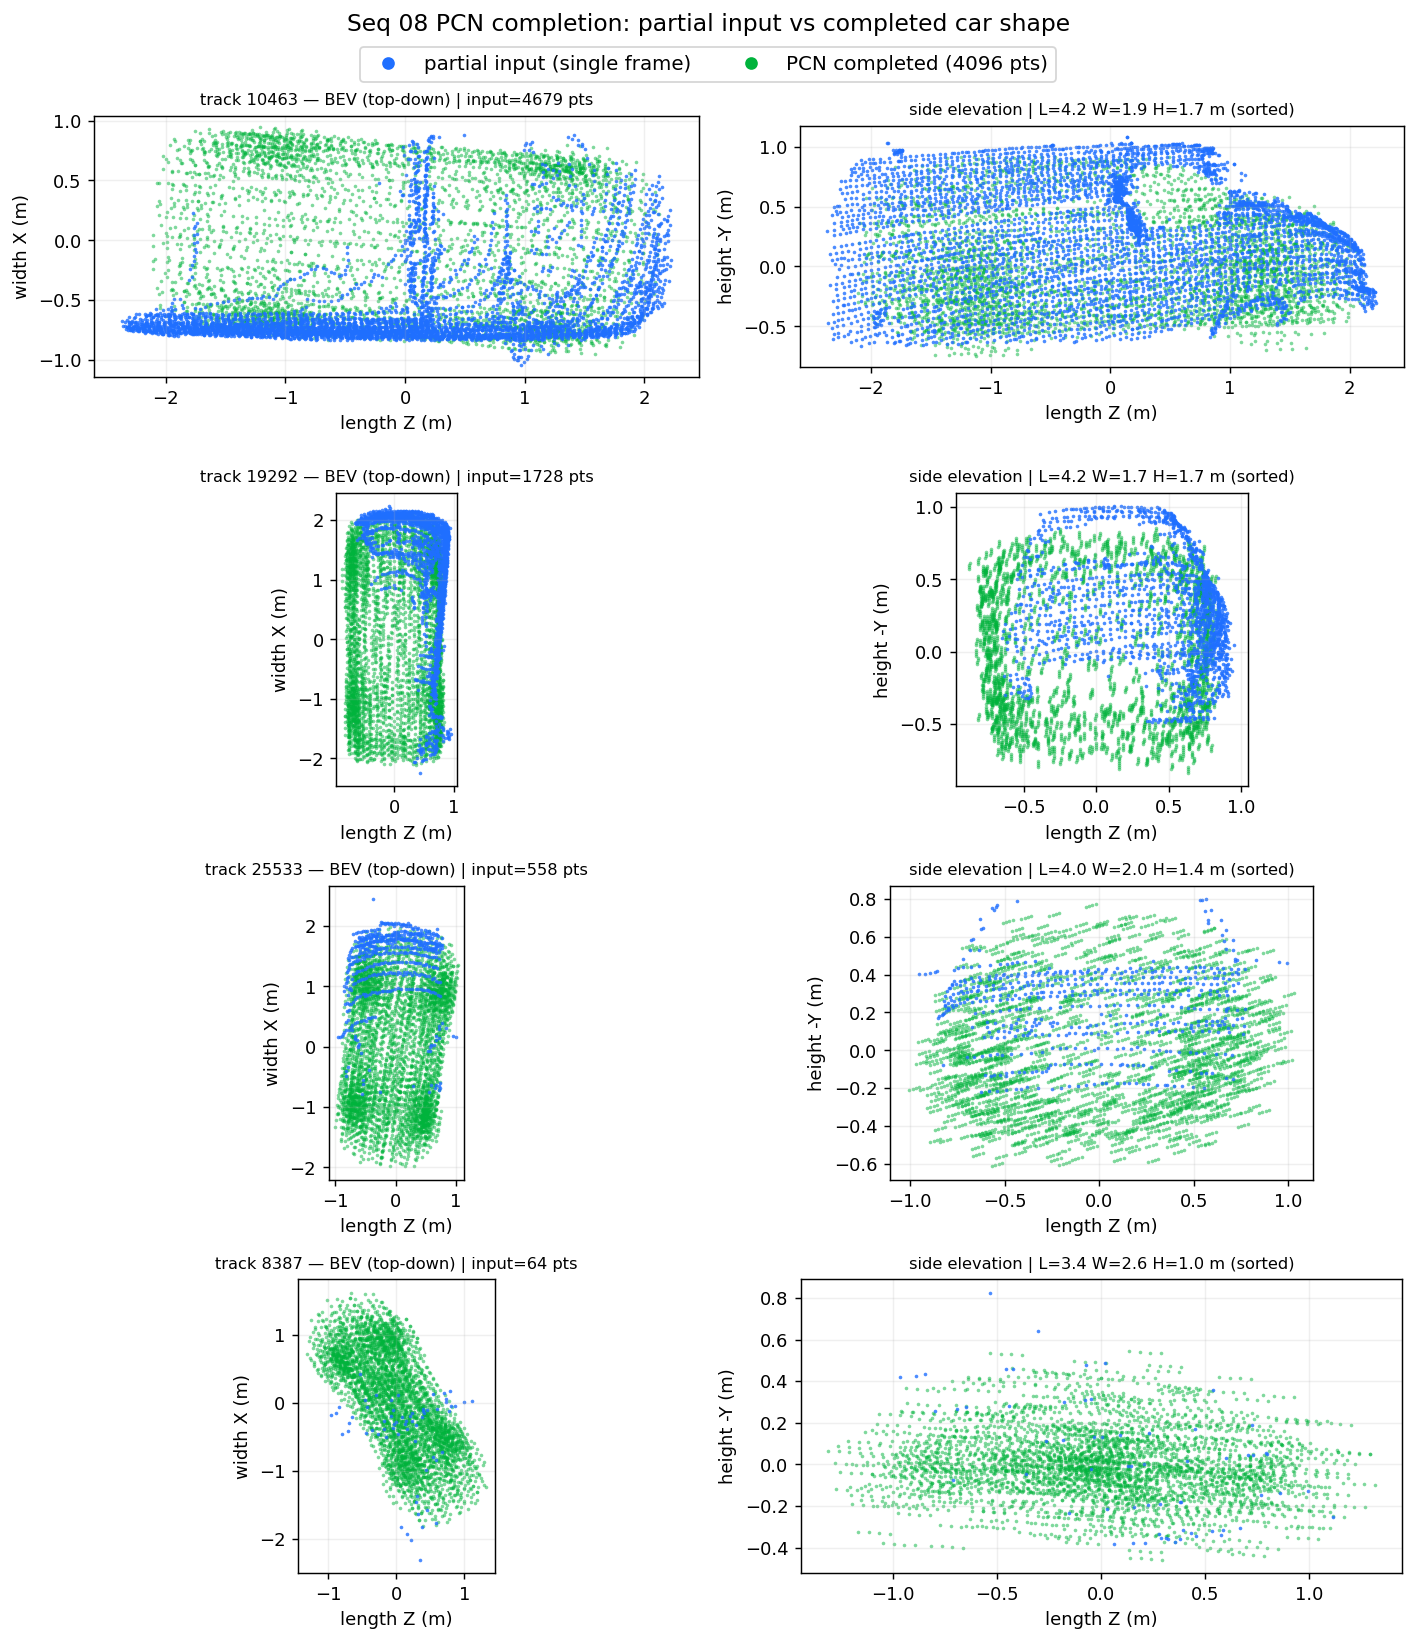
\includegraphics[width=\linewidth]{completion_shape_08.png}
  \caption[Completions on real seq-08 cars]{What the final completion path produces on real seq-08 cars, four
    tracks spanning the input-density range, each in the canonical car frame: bird's-eye
    view (left of each pair) and side elevation (right). Blue is the single-frame partial
    input, green the PCN completion. The completion recovers the full car footprint and a
    rough roofline silhouette from a one-sided partial; crispness and dimensional accuracy
    degrade on the sparsest inputs (the lowest-density car shows some width inflation).}
  \label{fig:completion-shape}
\end{figure}

\subsection{Negative Results and Lessons}
\label{sec:completion-lessons}

The method above was not reached in one step. Two false starts shaped it, and each
carries a lesson worth stating in its own right rather than smoothing over. They are
gathered here so that the method description reads as what the pipeline does. A third
intervention that was tried and rejected, a length-dependent far-end
compensation, is reported as a completion ablation
(Section~\ref{sec:abl-completion}).

\paragraph{The blobs were not a synthetic-data problem:}
\label{sec:completion-domaingap}
The first attempts to run PCN on real cars all produced ``blobs'', rounded,
car-sized clouds with no recognisable car structure. This was initially attributed to
the training data being synthetic, and the response was a series of sim-to-real
remedies: LiDAR-noise augmentation of the synthetic partials, and real-data
fine-tuning. None of them fixed the blobs, and the fine-tuning attempt is recorded as
a negative result, on this data, fine-tuning PCN on mined real pairs did not recover
real-car geometry. The blobs had two causes, and neither was the network weights: the
training-input distribution (Section~\ref{sec:completion-kittilike}) and the inference
normalisation (Section~\ref{sec:completion-normalisation}), the two method steps above.
The lesson is to suspect the data and the input pipeline before the model.

\paragraph{Train and inference semantics must match:}
\label{sec:completion-inferencebug}
Even after retraining on KITTI-like partials, real clusters still blobbed, and the
cause is the sharper lesson. An earlier inference path normalised each real partial by
a 3D PCA frame and the partial's own centroid and radius, a normalisation the
model had never seen, since it was trained in the canonical car frame of
Section~\ref{sec:completion-normalisation}. This silent train/inference mismatch alone
produced blobs, and it did so for every checkpoint, including in-distribution
synthetic ones where the model is otherwise clean. Because the two frames each looked
internally reasonable, the
divergence was invisible until measured. This incident is the motivating example for
the project's rule that any external integration or reuse gets a written semantics map
, coordinate frame, centring, and scale conventions, reconciled before code is
run.

\section{Summary and Methodological Limitations}
\label{sec:meth-limitations}

This chapter has set out the full method: the modular detection pipeline that turns a
raw scan into car detections, and the single-frame completion path with its input gate and
length prior. Several limitations are built into these choices and are flagged here so the
evaluation is read with them in view; each is taken up in full in the discussion of
Chapter~\ref{ch:conclusion}.

\begin{itemize}
  \item Ground model: a single global RANSAC plane assumes near-planar
    ground; it holds on the flat urban sequences used here but would degrade on
    strong slopes, where a grid-based model (future work) would be needed
    (Section~\ref{sec:pipeline-ground}).
  \item Offline by design: the tracker and track-level filter consult the
    whole sequence, and the pipeline runs far below sensor rate; real-time operation is
    out of scope (Section~\ref{sec:pipeline-overview}).
  \item Single-frame, static-car completion: completion runs on one frame's
    cluster; moving cars are completed but are considered separately, and no completion is
    scored against an accumulated multi-frame shape (Section~\ref{sec:completion-what}).
  \item Length-prior fallback: the per-car length estimate falls back to the
    fixed \SI{4.14}{\meter} prior on tracks with fewer than five gate-passed frames, and a
    residual far-end under-extension on long cars is a characterised, not eliminated, limit
    (Section~\ref{sec:completion-length}).
  \item Synthetic-only completion training: PCN sees only synthetic
    KITTI-like partials; real-data fine-tuning was a negative result, so a sim-to-real
    residual remains (Section~\ref{sec:completion-domaingap}).
\end{itemize}

With these caveats stated, Chapter~\ref{ch:evaluation} puts each component to the test
, the detection operating point and its ablations, the recall root-cause, and the
completion results (synthetic fidelity and independent-classifier plausibility), and
Chapter~\ref{ch:conclusion} returns to the limitations above alongside the evaluation
questions the results raise.


% ===== END inlined ch3_methodology.tex =====
% ===== BEGIN inlined ch4_evaluation.tex =====
% Chapter 4 -- Evaluation (\input by main.tex): detection protocol + detection results
% + recall analysis + completion results (synthetic CD/F + independent-classifier
% plausibility + reference-free fidelity). Merged from the former sec_4_1 /
% sec_4_results / sec_5 / sec_7_results fragments (seam markers below).
% Reframe (2026-09-12): the old self-made completion metric and box-reference evaluation
% removed; completion results rebuilt on synthetic fidelity + plausibility (Finding #54) + UCD/UHD.
%
% Honesty-phrasing rules applied (personal_agenda P1):
%   - "mean IoU" always qualified as "of matched detections"
%   - recall denominator stated explicitly (>=10 points surviving preprocessing)
%   - evaluation is leave-one-sequence-out (LOSO): each sequence is scored by a
%     classifier that never saw it in training or selection; seq 08 is the reported
%     operating point (fold-08 confirms the final seq-08 numbers)
%   - measured vs inferred evidence tiers marked in prose
%   - every number traceable to a finding / output artifact
%
\chapter{Experimental Evaluation}
\label{ch:evaluation}

This chapter evaluates the full pipeline end to end. It first fixes the
experimental setup, dataset, the pipeline under test, metrics, baselines, and
test environment (Section~\ref{sec:eval-protocol}). It then reports detection and
classification results together with runtime
(Section~\ref{sec:results-detection}), and the completion results, synthetic
fidelity, independent-classifier plausibility on real cars, and reference-free fidelity
(Section~\ref{sec:results-completion}). Two further
sections decompose these results: ablations that isolate each stage's
contribution (Section~\ref{sec:results-ablations}), and an analysis of where
detection succeeds and fails (Section~\ref{sec:recall-analysis}), which
root-causes the recall limit to the same clustering step that governs input
cleanliness for completion, the link between the chapter's two halves.

\section{Dataset}
\label{sec:eval-sequences}

The framework is grounded on two public datasets, matching its two halves.
SemanticKITTI~\cite{Behley_2019_ICCV} supplies the real Velodyne HDL-64E scans
used for detection, weak-label mining, and evaluation; its per-point semantic and instance
labels serve as ground truth. ShapeNetCore~v2~\cite{chang2015shapenetinformationrich3dmodel}
supplies the synthetic complete car meshes from which the completion network's training
partials are rendered (Section~\ref{sec:completion-kittilike}); no real car is ever
hand-labelled for completion. Detection and completion therefore draw on real and
synthetic data respectively, and the framework requires zero additional manual
annotation: the classifier's training data is auto-mined from existing semantic
annotations and the completion network is trained exclusively on synthetic shapes.

We evaluate on the eleven labelled SemanticKITTI odometry sequences
(\numrange{00}{10}), whose per-point semantic and instance labels serve as
ground truth. The official test sequences \numrange{11}{21} carry no
public labels, so no ground-truth detection metric can be computed on them; this
is a property of the dataset, not a choice, and it is why no labelled sequence
can be reserved as a conventional held-out test set. Table~\ref{tab:dataset} summarises
the labelled sequences, their frame counts, and their role in each half of the framework.

\begin{table}[H]
  \centering
  \caption[Labelled SemanticKITTI sequences and their roles]{The eleven labelled
    SemanticKITTI sequences (\numrange{00}{10}; \num{23201} labelled frames total), with
    per-sequence frame counts and their role. The binary classifier is trained on the ten
    non-08 sequences and validated on sequence~08; leave-one-sequence-out cross-validation
    (Section~\ref{sec:eval-loso}) re-partitions the same mined clusters so every sequence is
    scored by a classifier that never saw it. The completion network is trained only on
    synthetic ShapeNet partials and evaluated on all eleven sequences by
    independent-classifier plausibility (Section~\ref{sec:results-plausibility}).}
  \label{tab:dataset}
  \small
  \setlength{\tabcolsep}{5pt}
  \begin{tabular}{lccccccccccc}
    \toprule
    Seq & 00 & 01 & 02 & 03 & 04 & 05 & 06 & 07 & 08 & 09 & 10 \\
    \midrule
    Frames & 4541 & 1101 & 4661 & 801 & 271 & 2761 & 1101 & 1101 & 4071 & 1591 & 1201 \\
    Classifier role & \multicolumn{8}{c}{train} & val & \multicolumn{2}{c}{train} \\
    \bottomrule
  \end{tabular}
\end{table}

\paragraph{Train, validation, and test split:} For classification, the binary car/
not-car classifier is trained on the mined clusters of sequences \numrange{00}{07}, 09, and
10 and validated on sequence~08; the leakage-controlled result is the LOSO cross-validation
across all eleven sequences (Section~\ref{sec:eval-loso}). For completion, the PCN
network is trained on synthetic KITTI-like ShapeNet-car partials, with no real-data split,
and is evaluated on all eleven labelled sequences through the independent-classifier
plausibility protocol (Section~\ref{sec:results-plausibility}). The SemanticKITTI test
sequences (\numrange{11}{21}) are unusable for either, as they carry no public labels.

\paragraph{Classifier evaluation uses leave-one-sequence-out cross-validation:}
Rather than report detection on the sequence the classifier was tuned against, we
evaluate the binary classifier under leave-one-sequence-out (LOSO)
cross-validation over all eleven sequences. For each held-out sequence~$K$ a
classifier is trained on the other ten sequences and then run on the full
sequence~$K$; the held-out sequence contributes zero clusters to that
fold's training data and is never used to select the checkpoint. Checkpoint
selection is removed entirely: every fold trains for a fixed \num{15}-epoch
budget and the last-epoch checkpoint is used (historically the best epoch was
\num{13}/\num{15}, so last~$\approx$~best), so the held-out sequence is untouched
during both training and model selection. In the per-fold table below,
therefore, the classifier scoring sequence~$K$ has never seen
sequence~$K$ during training or model selection. Because the
Stage~B clusters are stored with a sequence prefix in their filenames, the folds
are a re-partition of the existing mined data and require no re-mining.

\paragraph{Two sequences carry additional, distinct roles:}
\begin{itemize}
  \item Sequence 08 (reported operating point; \num{4071} frames). The
    largest labelled sequence is the operating point at which the pipeline is
    reported in detail: the stage ablations (Section~\ref{sec:results-ablations}),
    the recall root-cause analysis (Section~\ref{sec:recall-analysis}), and the
    IoU-threshold sensitivity below are all computed on the sequence-08 output of the
    final classifier, and the completion constants were tuned on it (the completion
    evaluation itself, Section~\ref{sec:completion-results}, spans all eleven
    sequences). Sequence~08 was never used to tune the classical stages. The final
    classifier was historically selected on sequence~08, so its sequence-08 numbers
    could in principle be optimistic; the LOSO fold-08 classifier (trained on
    \numrange{00}{07},\,\numrange{09}{10}, last-epoch, never selected on 08) settles
    this empirically below.
  \item Sequence 00 (classifier training split, tuning baseline).
    Sequence~00's classical pipeline parameters (\texttt{PIPELINE\_CONFIG}) were
    historically hand-tuned on it, and it also sits in the classifier's training split,
    so its detection recall reads optimistically; we isolate that residual in the
    LOSO aggregate below (dropping fold-00 moves pooled recall by \num{0.022}). This does
    not touch the completion evaluation, which is a paired raw-versus-completed comparison
    on identical inputs and whose network never saw any real sequence.
\end{itemize}

\paragraph{Ground-truth targets and the eligibility rule:}
\label{sec:eval-targets}

The pipeline is a car detector, so the evaluation counts only the two
car-bearing SemanticKITTI classes as valid ground-truth objects:
car (class~10) and moving-car (class~252); we refer to this target
set as supported-vehicles. A ground-truth car instance is a
maximal set of points sharing one instance id within these classes.

An instance is counted in the evaluation only if at least 10 of its
points survive preprocessing, the $z$-filter, voxel downsampling, statistical
denoising, and ground removal that every scan passes through before clustering.
This is the recall denominator: recall is computed against ground-truth car
instances with $\geq 10$ points surviving preprocessing, not against every
annotated car. The rule exists because an instance reduced to a handful of points
by occlusion or range cannot be segmented by any clustering method, so including
it would measure sensor sparsity rather than the pipeline.

This choice narrows the denominator, and honesty requires quantifying by how
much. On a stride-20 sample of sequence~08 (204 of \num{4071} frames, drawn
uniformly across the drive), of all annotated car instances
(\num{2332} pooled), 25.5\% are excluded by the surviving-points rule;
measured instead against instances that have $\geq 10$ points in the raw
scan (\num{2033} pooled), 14.6\% are excluded by preprocessing.\footnote{%
These are two distinct $\geq 10$-point rules: one thresholds raw label
points (a distinct-car count), the other thresholds points surviving
preprocessing (the eval denominator). They are not interchangeable.}
Because an excluded instance can never be matched, the sequence-08 operating-point
recall of \num{0.732} against the eligible denominator corresponds, by inference, to a
recall of approximately \num{0.55} against all annotated cars
(the eligible-to-annotated survival ratio on this sample is
$\num{1737}/\num{2332}=\num{0.745}$; the ratio is a stride-20 estimate, so this
figure is inferred, not separately measured). We report the eligible-denominator
recall as the headline and disclose the all-annotated figure alongside it.

\section{Experimental Setup}
\label{sec:eval-protocol}

Every quantitative claim about detection in this thesis is produced by a single
evaluation script under one fixed protocol. Because
the results, ablation, and recall-analysis sections all report numbers from this
protocol, we state it in full here and refer back to it rather than restating it
per table. The protocol was frozen before the write-up began; no configuration,
checkpoint, or metric definition described below was altered to produce a
reported number.

\subsection{Baseline Methods}
\label{sec:eval-baselines}

Detection is not compared head-to-head against the supervised networks of
Section~\ref{sec:bg-positioning}: those report different metrics under different
protocols, and Table~\ref{tab:positioning} sets out that non-comparison and the
paradigm gap behind it. Within this pipeline the classical stages and the track
filter are instead compared against one another by ablation
(Section~\ref{sec:results-ablations}). Completion is judged against explicit
references on the same inputs: the raw partial (the paired baseline the
completion must beat), a dense static-accumulation ceiling (the shape-quality
upper bound of a correctly-shaped car), and, for architecture, PoinTr. Real-data
completion quality is scored by the independent-classifier plausibility of
Section~\ref{sec:results-plausibility}, with the standard reference-free metrics UCD and
UHD (Section~\ref{sec:bg-completion}) reported alongside it in
Section~\ref{sec:results-fidelity}.

\subsection{Evaluation Metrics}
\label{sec:eval-matching}

Detections and ground-truth instances are compared at the point level.
For a detection mask $D$ and an instance mask $G$ over the surviving points, the
overlap is the intersection-over-union
\[
  \mathrm{IoU}(D,G) \;=\; \frac{|D \cap G|}{|D \cup G|}.
\]
All detection--instance pairs with $\mathrm{IoU} \geq \tau$ are collected, sorted
by descending IoU, and assigned greedily and one-to-one: the highest-IoU
pair is matched first, and once a detection or an instance is used it cannot be
matched again. This yields, per frame:
\begin{itemize}
  \item a true positive (TP) for each matched pair,
  \item a false positive (FP) for each unmatched detection,
  \item a false negative (FN) for each unmatched eligible instance.
\end{itemize}
Precision, recall, and $F_1$ are then computed from TP, FP, and FN
micro-averaged over the sequence: counts are pooled across all frames and
the ratios taken once, so denser frames contribute proportionally more. We also
report the mean IoU of matched detections, the mean of the IoU values
of the accepted TP pairs only. This is a quality measure of the matches that were
made; it says nothing about missed cars and must not be read as an overall
segmentation score.

Track-level filtering is enabled by default for the headline numbers: an offline
centroid tracker links detections across frames, and only tracks meeting a
minimum length and class-consistency requirement are accepted. This is a
post-hoc, offline step (it uses the whole sequence), consistent with the
offline scope of the system; its effect is isolated as an ablation row in the
ablation section (Section~\ref{sec:results-ablations}).

\paragraph{Choice of IoU threshold and its sensitivity:}
\label{sec:eval-iou-threshold}

All headline numbers use $\tau = 0.3$. A point-level threshold of 0.3 is
permissive relative to the bounding-box 0.5 common in detection benchmarks, so
it is fair to ask whether the results are an artifact of a lenient gate. They
are not, and the reason is visible in Table~\ref{tab:headline}: the mean IoU of
matched detections is \num{0.913} on sequence~08, far above either threshold, so
the matches are not marginal overlaps sitting just past $\tau$.

To make this concrete we re-ran the full sequence~08 evaluation at
$\tau \in \{0.25, 0.30, 0.50\}$ with everything else frozen
(Table~\ref{tab:iou-sensitivity}).

\begin{table}[H]
  \centering
  \caption[IoU-threshold sensitivity on seq~08]{IoU-threshold sensitivity on the full sequence~08 (frozen
    configuration). The $\tau = 0.30$ row is the headline. $F_1$ moves by at most
    \num{2.7} points across the tested range (\num{0.815} at $\tau=0.25$ to
    \num{0.788} at $\tau=0.50$); mean IoU of matched detections rises at the
    stricter gate because it keeps only the better-overlapping matches.}
  \label{tab:iou-sensitivity}
  \begin{tabular}{cccccc}
    \toprule
    $\tau$ & Precision & Recall & $F_1$ & Mean IoU & TP / FP / FN \\
    \midrule
    0.25 & 0.914 & 0.735 & 0.815 & 0.910 & \num{25660} / \num{2421} / \num{9262} \\
    0.30 & 0.911 & 0.732 & 0.812 & 0.913 & \num{25568} / \num{2513} / \num{9354} \\
    0.50 & 0.884 & 0.711 & 0.788 & 0.927 & \num{24837} / \num{3244} / \num{10085} \\
    \bottomrule
  \end{tabular}
\end{table}

$F_1$ falls only \num{2.4} points from the headline $\tau = 0.30$ to the strict
$\tau = 0.50$ (\num{0.812} to \num{0.788}), and \num{2.7} points across the full
tested range from the permissive $\tau = 0.25$ (\num{0.815}), so the reported
quality is stable under the choice of threshold and does not depend on the lenient
value. We had
pre-registered that a threshold-sensitive result would be reported as a
finding rather than tuned away; it was not sensitive.


%% ===== merged from sec_4_results.tex ===== %%

% Detection Results, Ablations, Range, Runtime (Sections 4.2--4.5; folds under Chapter 4).
% Opens with \section{Detection Evaluation} carrying its own distinct label
% (\label{ch:detection-eval-results}), which does not clash with the chapter's
% \label{ch:evaluation}.
%
% Honesty-phrasing rules applied (personal_agenda P1):
%   - "mean IoU" always qualified as "of matched detections"
%   - recall denominator restated / cross-referenced (>=10 surviving points)
%   - seq 08 = classifier model-selection set, not a held-out test set
%   - negative results reported AS FINDINGS, not apologised for
%     (C5 synthetic-pretraining redundant; clustering "adopt nothing")
%   - the distance table is per-frame / track-filter-OFF: stated as a deviation,
%     read as a trend, NOT a restatement of the 0.732 headline
%   - every number traces to a finding / output artifact (cited Finding~\#NN)
%
\subsection{Implementation Details}
\label{sec:eval-pipeline}

The system under evaluation is the frozen detection-and-completion pipeline of
Chapter~\ref{ch:pipeline}, run unmodified by a single script:
ground removal, HDBSCAN clustering, the geometric
filter, the binary classifier, and the centroid tracker with its track-level
filter for detection; and, for each detected car, the KITTI-like-trained PCN
behind the L-shape input gate for completion. Every number below uses the
committed \texttt{PIPELINE\_CONFIG} (Table~\ref{tab:pipeline-config}); no stage,
checkpoint, or parameter was changed to obtain a reported result.

The framework's defining property is that supervision is confined to two learned stages,
with all geometric reasoning done by training-free classical methods
(Table~\ref{tab:sup-unsup}). This is what lets the framework require zero additional
manual annotation: the classical stages need no training data at all, the classifier is
trained on supervision auto-mined from existing semantic annotations, and the
completion network on synthetic ShapeNet partials.

\begin{table}[H]
  \centering
  \caption[Unsupervised and supervised stages of the framework]{The framework's stages by
    supervision. The six unsupervised stages are training-free classical methods; the two
    supervised stages are learned but require no additional manual annotation (the classifier
    is trained on supervision auto-mined from existing semantic annotations, the completion
    network on synthetic ShapeNet partials).}
  \label{tab:sup-unsup}
  \small
  \begin{tabular}{@{}p{0.46\linewidth}p{0.46\linewidth}@{}}
    \toprule
    Unsupervised (classical, training-free) & Supervised (learned, no real labels) \\
    \midrule
    $z$-filter; denoise + voxel downsample; RANSAC ground removal; HDBSCAN clustering;
      geometric OBB filter; centroid tracker + track-level filter
      & Binary car/not-car PointNet classifier (mined weak labels); PCN completion
      (synthetic ShapeNet partials) \\
    \bottomrule
  \end{tabular}
\end{table}

\label{sec:eval-environment}
All runs are deterministic: ground-plane RANSAC and the classifier use fixed
seeds (Chapter~\ref{ch:pipeline}), so a rerun reproduces every reported number.
Timings are wall-clock on an AMD Ryzen~7 7800X3D with an RTX~3070~Ti, measured on
the full sequence~08 under the promoted configuration
(Section~\ref{sec:results-runtime}). The classifier and PCN training
hyperparameters, optimiser, learning-rate schedule, epochs, and batch size,
are given with each model in Chapter~\ref{ch:pipeline} and are not repeated here.

\section{Detection and Classification Results}
\label{sec:results-detection}

\subsection{The Reported Operating Point on Sequence 08}
\label{sec:eval-operating-point}

Table~\ref{tab:headline} gives the reported operating point on the full
sequence~08 under this protocol, produced by the final classifier (the one the
completion pipeline actually runs with). This is the operating point the
ablation and recall-analysis sections of this chapter decompose; the
cross-validation that confirms it follows in Section~\ref{sec:eval-loso}.

\begin{table}[H]
  \centering
  \caption[Reported detection operating point]{Reported detection operating point on the
    full sequence~08 (frozen protocol, final classifier), with its leave-one-sequence-out
    held-out counterpart, fold-08, a classifier that never saw sequence~08
    (Section~\ref{sec:eval-loso}). The two agree on recall (the held-out row is marginally
    higher) and differ by about two precision points, so selecting the classifier on
    sequence~08 did not inflate the reported recall. Sequence~08 is the largest labelled
    sequence and was never used to tune the classical stages; mean IoU is over matched
    detections only.}
  \label{tab:headline}
  \setlength{\tabcolsep}{5pt}
  \begin{tabular}{lccccc}
    \toprule
    Classifier (seq~08) & Precision & Recall & $F_1$ & Mean IoU & TP / FP / FN \\
    \midrule
    Reported (final)        & 0.911 & 0.732 & 0.812 & 0.913 & \num{25568} / \num{2513} / \num{9354} \\
    Held-out (LOSO fold-08) & 0.888 & 0.736 & 0.805 & 0.913 & \num{25715} / \num{3228} / \num{9207} \\
    \bottomrule
  \end{tabular}
\end{table}

The pipeline is precision-saturated and recall-limited: false positives are flat
at roughly one per frame, while recall is set by how many eligible cars the
clustering stage recovers as single objects. The remaining sections of this
chapter report the ablations that decompose this operating point, and Section~\ref{sec:recall-analysis}
root-causes the recall shortfall.

\subsection{Per-Frame Detection Results}

The headline operating point is the reported row of Table~\ref{tab:headline}
(Section~\ref{sec:eval-protocol}): precision \num{0.911}, recall \num{0.732}, $F_1$ \num{0.812}, and
a mean IoU of matched detections of \num{0.913}, over
\num{25568}~/~\num{2513}~/~\num{9354} TP~/~FP~/~FN. Two properties of this
operating point organise the rest of the chapter, and both are visible directly
in the per-frame record rather than only in the pooled totals.

First, the pipeline is precision-saturated. Across the full sequence the
false-positive count is low and stable, about \num{0.6} per frame
(\num{2513} over \num{4071} frames), independent of how many cars are in view.
Figure~\ref{fig:bev-detections} shows this spatially, detections track the
true parked and moving cars along the street, with few spurious boxes, and
Figure~\ref{fig:timeseries} shows it over time: the FP trace is low and
stationary while the number of ground-truth cars per frame swings widely.

Second, the pipeline is recall-limited, and the limit is structural. The
recall shortfall traces to a measured clustering failure: HDBSCAN splits large,
close cars into fragments that no longer match a single instance, and the split rate is highest exactly where cars are densest and
nearest (\SI{53.5}{\percent} at \SIrange{0}{10}{\metre}).
Section~\ref{sec:results-distance} exhibits the resulting near-range recall dip
directly, and the time series (Figure~\ref{fig:timeseries}) shows per-frame
recall tending to fall in the denser frames while false positives stay flat. We
root-cause the splitting mechanism in Section~\ref{sec:recall-analysis}; here we establish only that
recall, not precision, is the dominant error mode, and that it does not come from
the classifier misfiring (false positives stay flat regardless).

\begin{figure}[htbp]
  \centering
  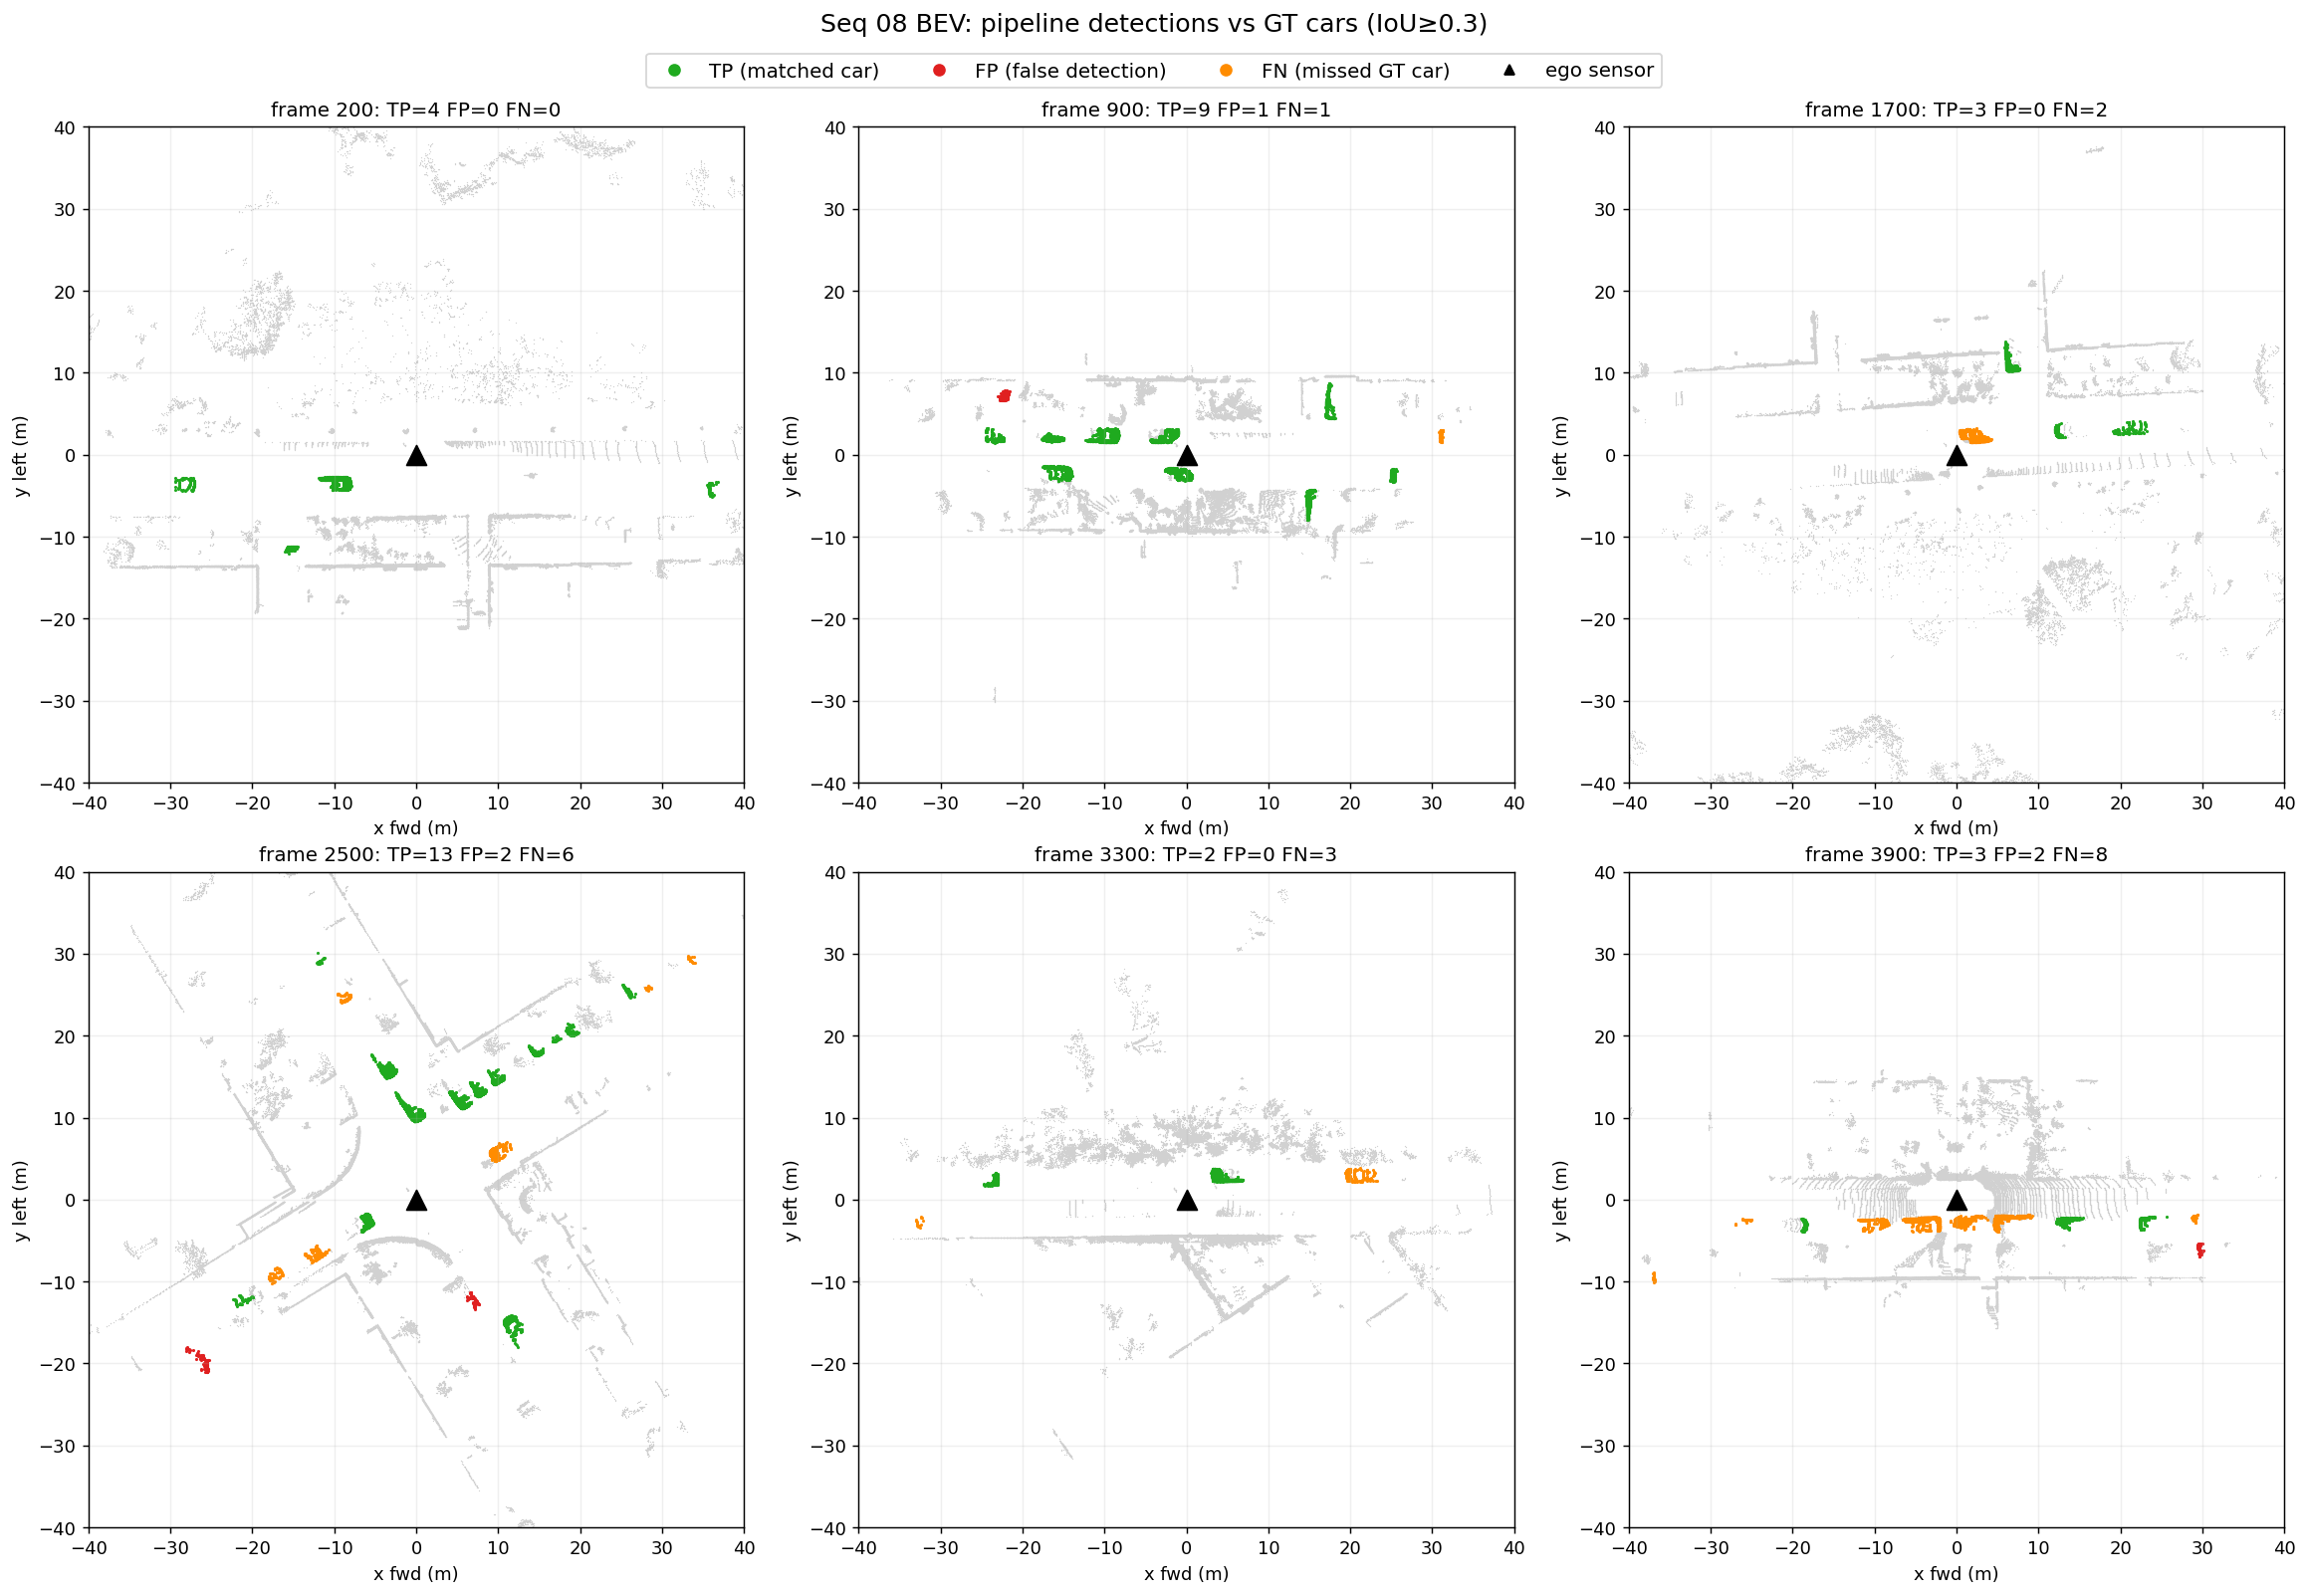
\includegraphics[width=\linewidth]{seq08_bev_detections.png}
  \caption[Bird's-eye view of detections on seq~08]{Bird's-eye view of detections on a representative sequence~08 frame.
    Detected car clusters (coloured) are overlaid on the ground-removed point
    cloud; ego is at the origin. Detections concentrate on true vehicles, with
    few spurious clusters, the precision-saturated behaviour reported in
    Table~\ref{tab:headline}.}
  \label{fig:bev-detections}
\end{figure}

\begin{figure}[htbp]
  \centering
  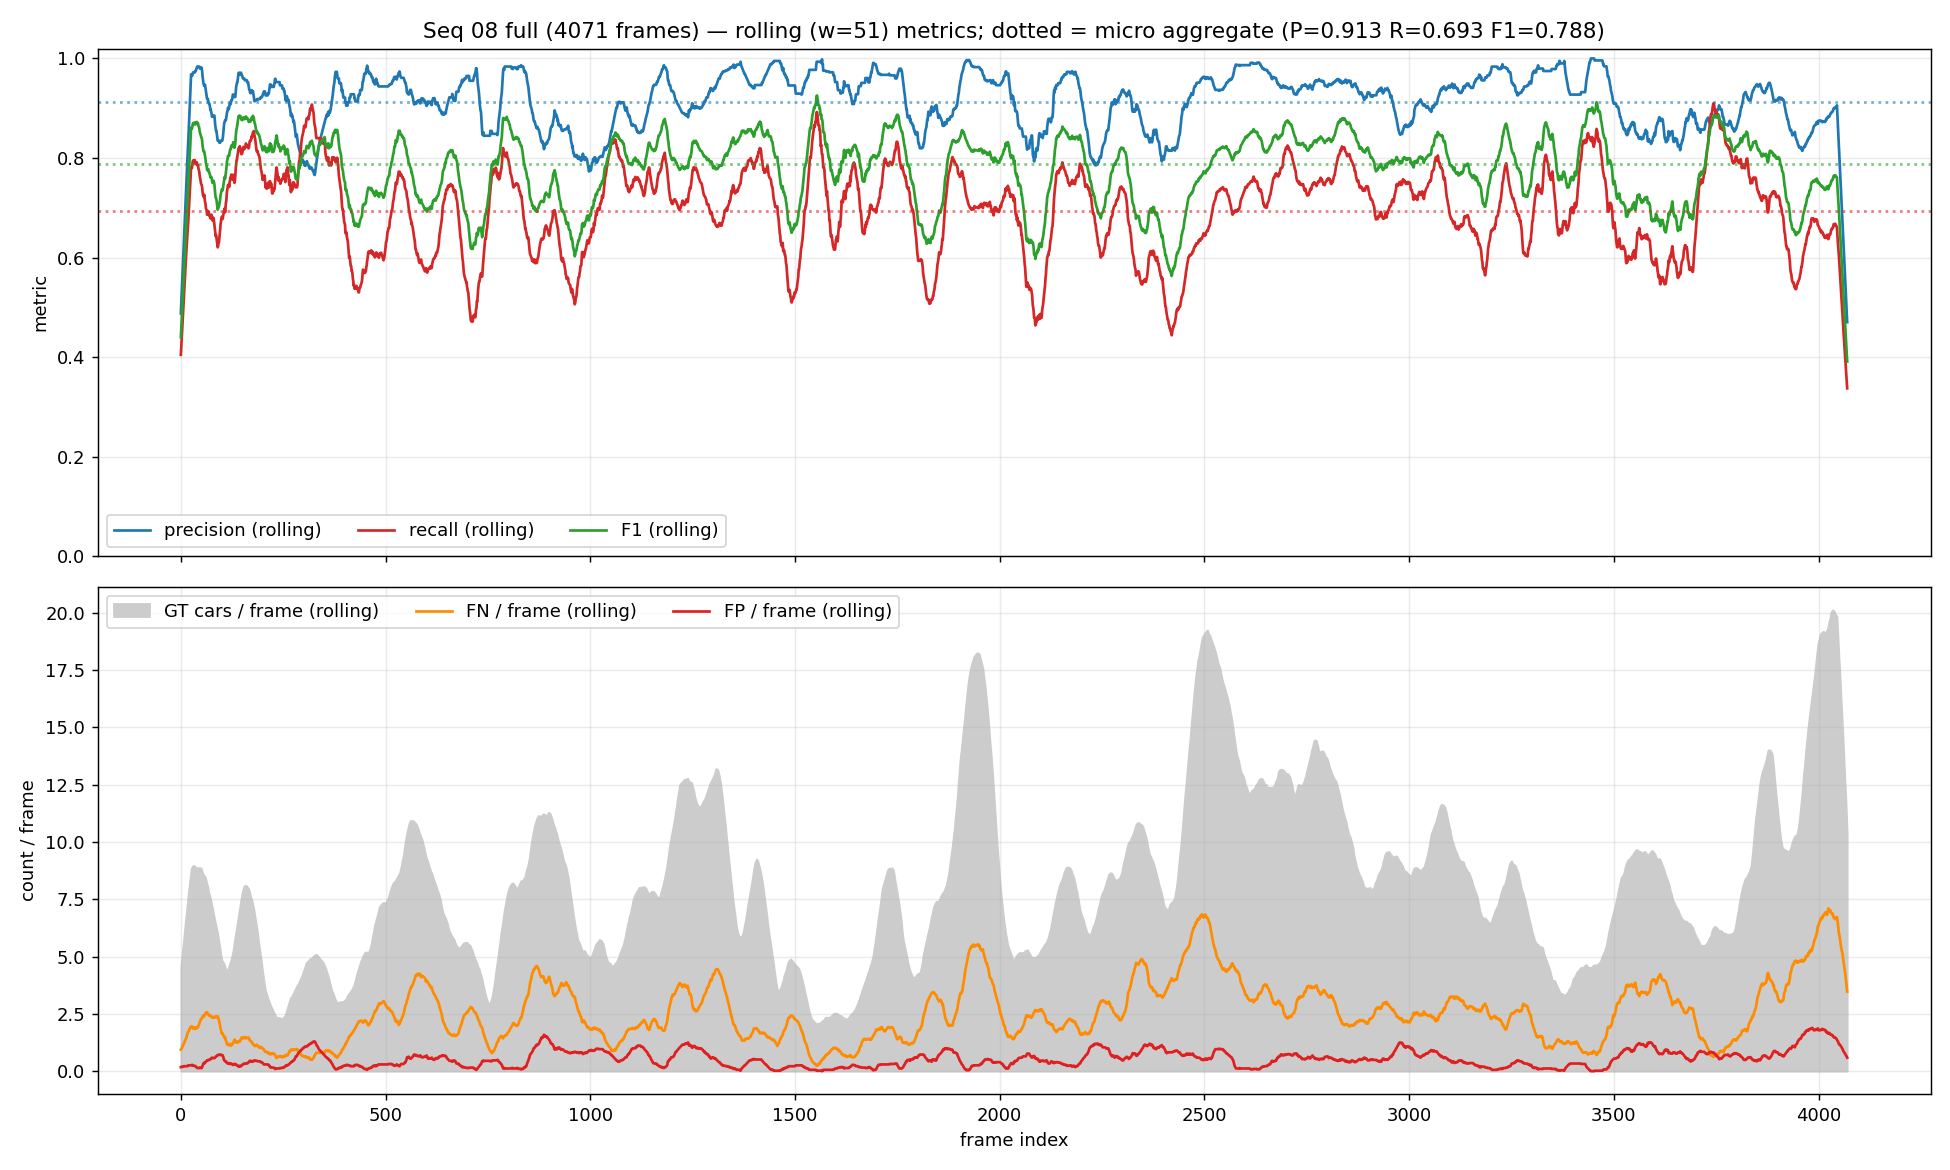
\includegraphics[width=\linewidth]{seq08_timeseries.png}
  \caption[Per-frame detection behaviour on seq~08]{Per-frame detection behaviour over sequence~08. False positives (lower
    trace) stay low and flat, under one per frame, regardless of scene
    content, while per-frame recall tends to fall in frames with more
    ground-truth cars. The structural recall limit is root-caused in Section~\ref{sec:recall-analysis}
    (HDBSCAN splitting).}
  \label{fig:timeseries}
\end{figure}

\subsection{Leave-One-Sequence-Out Cross-Validation}
\label{sec:eval-loso}

The operating point above is reported on sequence~08, which is also the sequence
the final classifier was historically selected on. To show that this selection
does not inflate the result, and to characterise the per-sequence recall spread
that a single reporting sequence cannot, we ran the LOSO protocol of
Section~\ref{sec:eval-sequences}: eleven folds, each training a classifier on ten
sequences and evaluating the full held-out eleventh, so every fold's classifier
is blind to the sequence it scores. Table~\ref{tab:loso} reports all eleven folds,
the pooled micro-average (counts summed across folds, comparable to the single
operating-point number), and the macro mean~$\pm$~standard deviation across folds.

\begin{table}[H]
  \centering
  \caption[Leave-one-sequence-out cross-validation]{Leave-one-sequence-out cross-validation over all eleven labelled
    sequences (full sequences, $\tau=0.3$, final configuration). Each fold's
    classifier trained on the other ten sequences and was never selected on the
    held-out one, so no row's classifier has seen the sequence it scores.
    ``Pooled'' sums TP/FP/FN across folds; the excl.-seq00 pool isolates the
    residual seq-00 classical-tuning familiarity (Section~\ref{sec:eval-sequences}).}
  \label{tab:loso}
  \setlength{\tabcolsep}{3pt}
  \footnotesize
  \begin{tabular}{lccccc}
    \toprule
    Held-out seq & Precision & Recall & $F_1$ & Mean IoU & TP / FP / FN \\
    \midrule
    00 (\num{4541} fr.) & 0.921 & 0.758 & 0.831 & 0.933 & \num{42583} / \num{3675} / \num{13607} \\
    01 (\num{1101} fr.) & 0.957 & 0.336 & 0.498 & 0.953 & \num{540} / \num{24} / \num{1066} \\
    02 (\num{4661} fr.) & 0.823 & 0.701 & 0.757 & 0.904 & \num{10941} / \num{2345} / \num{4663} \\
    03 (\num{801} fr.)  & 0.796 & 0.623 & 0.699 & 0.905 & \num{1528} / \num{391} / \num{925} \\
    04 (\num{271} fr.)  & 0.824 & 0.510 & 0.630 & 0.836 & \num{539} / \num{115} / \num{517} \\
    05 (\num{2761} fr.) & 0.880 & 0.725 & 0.795 & 0.910 & \num{10585} / \num{1448} / \num{4013} \\
    06 (\num{1101} fr.) & 0.873 & 0.637 & 0.737 & 0.906 & \num{6379} / \num{931} / \num{3632} \\
    07 (\num{1101} fr.) & 0.916 & 0.726 & 0.810 & 0.930 & \num{11089} / \num{1011} / \num{4179} \\
    08 (\num{4071} fr.) & 0.888 & 0.736 & 0.805 & 0.913 & \num{25715} / \num{3228} / \num{9207} \\
    09 (\num{1591} fr.) & 0.851 & 0.638 & 0.729 & 0.913 & \num{5072} / \num{888} / \num{2882} \\
    10 (\num{1201} fr.) & 0.745 & 0.557 & 0.638 & 0.872 & \num{1826} / \num{625} / \num{1450} \\
    \midrule
    \textbf{Pooled (all 11)} & \textbf{0.888} & \textbf{0.717} & \textbf{0.793} & \textbf{0.919} & \num{116797} / \num{14681} / \num{46141} \\
    Pooled (excl.\ seq~00)   & 0.871 & 0.695 & 0.773 & 0.912 & \num{74214} / \num{11006} / \num{32534} \\
    Macro mean $\pm$ std     & $0.861{\pm}0.059$ & $0.632{\pm}0.119$ & $0.721{\pm}0.095$ & $0.907{\pm}0.030$ &, \\
    \bottomrule
  \end{tabular}
\end{table}

Three things follow. First, model selection did not inflate the reported
recall. The fold-08 classifier, blind to sequence~08, reaches recall \num{0.736} against
the sequence-08 operating point's \num{0.732}, if anything marginally higher,
not lower, so the recall headline is not a product of having selected the
classifier on the reporting sequence. The model-selection optimism that does
exist is confined to precision and is small: fold-08 precision is \num{0.888}
versus the final \num{0.911} (an extra \num{715} false positives across
\num{4071} frames), exactly the two-point, precision-only exposure the stage
decomposition predicts (Section~\ref{sec:disc-eval-validity}). The two
sequence-08 rows are not two separate experiments but one classifier under
two checkpoint-selection rules: the final model and the fold-08 model share the
same architecture, the same ten training sequences (\numrange{00}{07},
\numrange{09}{10}), and the same from-scratch \num{15}-epoch regime, and differ
only in which epoch is frozen, the final model takes the epoch that scored
best on the sequence-08 validation set, the fold-08 model takes the last epoch and
never inspects sequence~08 at all. The \num{0.732}~$\rightarrow$~\num{0.736}
(recall) and \num{0.911}~$\rightarrow$~\num{0.888} (precision) deltas therefore
isolate the effect of that selection: selecting on sequence~08 bought about two
precision points and no recall. The isolation is not perfect, because
sequence~08 cannot serve as the fold's loss-monitoring split, the fold-08 model
trains on \SI{95}{\percent} of the final model's clusters (a \num{5}-percent
monitoring slice is set aside), but that confound removes training data from
the fold-08 model, which would depress its recall, not inflate it, so it only
strengthens the ``recall was not inflated'' reading. Second, the
pooled cross-validated operating point over all eleven sequences,
precision \num{0.888}, recall \num{0.717}, $F_1$~\num{0.793}, mean IoU
\num{0.919}, sits within roughly two points of the sequence-08 operating point
on every metric, so the reported numbers are representative of the labelled set
and not specific to sequence~08. Third, the per-sequence spread is now
explicit: recall ranges from \num{0.336} on sequence~01 (a sparse highway drive)
to \num{0.758} on sequence~00 (dense urban), with a macro mean of
\num{0.632}~$\pm$~\num{0.119}; precision is far steadier
(\num{0.861}~$\pm$~\num{0.059}). The gap between the pooled recall (\num{0.717})
and the macro mean (\num{0.632}) is driven by the smallest, sparsest sequences
(seq~01 and seq~04, the latter only \num{271} frames), which the count-weighted
pool down-weights and the unweighted mean does not; both figures are reported so
neither hides the spread. Finally, the residual seq-00 classical-tuning exposure
is bounded: dropping the seq-00 fold lowers pooled recall only from \num{0.717}
to \num{0.695} (a \num{0.022} delta), so the historical seq-00 pipeline tuning
does not drive the aggregate.

\subsection{Detection Accuracy Versus Range}
\label{sec:results-distance}

Recall is not uniform in range, and the way it varies is not the naive
``far~=~worse'' monotone one might expect. Table~\ref{tab:distance} stratifies
detection by the range of each cluster's centroid from the ego sensor, on a
stride-20 sample of sequence~08 under the frozen configuration.
Deviation: like the clustering benchmark, this table is
per-frame with the track filter off (striding breaks the tracker), so its
pooled recall (\num{0.671}) is a per-frame figure and does not restate the
track-filtered headline \num{0.732}; read the table as a range trend, not
as a re-derivation of the headline.

\begin{table}[H]
  \centering
  \caption[Detection stratified by range-to-ego on seq~08]{Detection stratified by range-to-ego on sequence~08 (stride-20 sample,
    frozen configuration, per-frame / track-filter-off). Recall is
    non-monotonic: it dips in the nearest bin, peaks at
    \SIrange{10}{20}{\metre}, then falls with range. The nearest-bin dip is
    over-segmentation, the far decline is sparsity. Mean IoU is
    over matched detections. Summing the two near bins recovers the
    \SIrange{0}{20}{\metre} figure ($R=\num{0.829}$) comparable to the earlier
    range analysis.}
  \label{tab:distance}
  \begin{tabular}{lccccc}
    \toprule
    Range (m) & Precision & Recall & $F_1$ & Mean IoU (matched) & TP / FP / FN \\
    \midrule
    0--10   & 0.899 & 0.787 & 0.839 & 0.902 & \num{311} / \num{35}  / \num{84}  \\
    10--20  & 0.869 & \textbf{0.862} & 0.866 & 0.926 & \num{432} / \num{65}  / \num{69}  \\
    20--40  & 0.799 & 0.550 & 0.652 & 0.934 & \num{401} / \num{101} / \num{328} \\
    40+     & 0.512 & 0.196 & 0.284 & 0.943 & \num{22}  / \num{21}  / \num{90}  \\
    \midrule
    Pooled  & 0.840 & 0.671 & 0.746 & 0.923 & \num{1166} / \num{222} / \num{571} \\
    \bottomrule
  \end{tabular}
\end{table}

The counter-intuitive result is the nearest-bin recall dip: recall at
\SIrange{0}{10}{\metre} (\num{0.787}) is lower than at
\SIrange{10}{20}{\metre} (\num{0.862}), even though near cars carry far more
points. This is not sparsity, it is over-segmentation. The split-rate analysis shows
that HDBSCAN splits the majority of the very-near cars (a split rate of
\SI{53.5}{\percent} at \SIrange{0}{10}{\metre}, falling to \SI{3.5}{\percent} past
\SI{40}{\metre}): a large, close car dissolves into several clusters,
none of which matches the whole instance, so it is counted as a miss. The nearest bin
also has the lowest mean IoU of matched detections (\num{0.902}),
consistent with fragments eroding the overlap even on the cars that do match. We
develop this splitting mechanism, and why post-hoc fragment-merging fails to
recover it, in Section~\ref{sec:recall-analysis}.

Beyond the peak the decline is ordinary sparsity: recall falls from \num{0.862}
at \SIrange{10}{20}{\metre} to \num{0.550} at \SIrange{20}{40}{\metre} and
\num{0.196} past \SI{40}{\metre}, as cars thin to too few surviving points to
cluster or to clear the \num{10}-point eligibility rule (Section~\ref{sec:eval-protocol}).
Mean IoU of matched detections rises with range
(\num{0.902}~$\rightarrow$~\num{0.943}): the far cars that are detected at all are
compact, single-cluster instances, so their overlap is clean even as their number
collapses. The earlier precision-only, seq-00, pre-promotion range analysis is superseded by this on-frozen-config sequence-08 table and is
retained only as a historical note.

\section{Runtime Evaluation}
\label{sec:results-runtime}

Table~\ref{tab:runtime} breaks the per-frame cost down by stage, measured over
the full sequence~08 under the final (promoted) configuration
(\num{4068} timed frames, RTX~3070~Ti / Ryzen~7~7800X3D;
per-stage figures from \texttt{timing\_seq08\_full\_n4068\_combined.json}). The breakdown shows where
the time goes: the two classical geometric stages, ground-plane RANSAC and,
above all, HDBSCAN clustering, dominate, together taking roughly
\SI{68}{\percent} of the frame; adding preprocessing and the geometric filter,
the classical CPU stages account for about \SI{94}{\percent}, leaving the single
learned component, the classifier, at only $\sim$\SI{5.4}{\percent} (the
centroid/Hungarian tracker is a classical assignment step, not learned). The
classifier is \SI{33.7}{\milli\second} for the $\sim$\num{45} clusters in a frame
($\sim$\SI{0.75}{\milli\second} each) and the tracker is negligible.

\begin{table}[H]
  \centering
  \caption[Per-frame runtime by stage on seq~08]{Per-frame runtime by stage on the full sequence~08 under the final
    (promoted) configuration (\num{4068} timed frames; mean ms).
    Clustering alone is nearly \SI{60}{\percent} of the frame. The total is
    $\approx\SI{623.5}{\milli\second}$ ($\approx$\num{1.6}~fps) on this full run;
    a stride-20 sample of the same configuration estimates
    $\approx\SI{650.6}{\milli\second}$ (the two agree to within the sampling
    variation of the expensive stages). The pre-optimisation configuration
    totalled \SI{921.3}{\milli\second}. Percentages are of the
    \SI{623.5}{\milli\second} total.}
  \label{tab:runtime}
  \begin{tabular}{lcc}
    \toprule
    Stage & Mean (ms) & Share \\
    \midrule
    Data load                       & 0.7   & 0.1\% \\
    Preprocessing (z-filter, denoise, voxel) & 125.9 & 20.2\% \\
    Ground removal (RANSAC)         & 56.2  & 9.0\% \\
    Clustering (HDBSCAN)            & 370.4 & 59.4\% \\
    Geometric filter                & 36.2  & 5.8\% \\
    Classification                  & 33.7  & 5.4\% \\
    Tracking                        & 0.3   & 0.1\% \\
    \midrule
    Total                           & 623.5 & 100\% ($\approx$1.6 fps) \\
    \bottomrule
  \end{tabular}
\end{table}

The promoted configuration is itself the product of a runtime optimisation that
targeted the dominant classical stages directly: reducing the
RANSAC iteration count and coarsening the clustering voxel to \SI{0.10}{\metre}
cut the per-frame total by roughly a third, from a pre-optimisation
\SI{921.3}{\milli\second} to \SI{623.5}{\milli\second} on the full sequence
(\SI{650.6}{\milli\second} on the stride-20 sample), and the coarser voxel also
improved detection, it is the promoted configuration used throughout
this chapter. A sub-\SI{400}{\milli\second} target was shown to be unreachable
through the authorised optimisation tiers, the post-ground object cloud is
intrinsically sparse, so coarser voxelisation compresses it little and the Python
HDBSCAN retains a floor of $\sim$\SI{185}{\milli\second}, and the achieved
operating point was accepted, real-time operation being out of scope (user
decision, \num{2026}-07-23). Point-completion, when it runs, adds
$\sim$\SI{13}{\milli\second} per completed car on top of detection and is not part
of the detection budget above.


%% ===== merged from sec_5_recall_bottleneck.tex ===== %%

% The Recall Bottleneck (folds under Chapter 4 as a section, not a chapter of its own).
% Root-causes the recall shortfall established earlier in the chapter and reports the
% failed repair strategies as a negative-results contribution. Sub-tables are
% referenced by section + Finding number rather than hard-coded table number, to stay
% robust to renumbering.
%
% Honesty-phrasing rules applied (personal_agenda P1):
%   - recall denominator restated / cross-referenced (>=10 surviving points, Sec 4.1)
%   - "mean IoU" always qualified as "of matched detections"
%   - negative results (#21/#24, temporal aggregation) reported AS FINDINGS, not
%     apologised for
%   - the retracted "~0.74 hard limit" is corrected explicitly (#24 Correction / #34)
%   - two measurement eras kept separate: the pre-promotion seq-00 repair search
%     (baseline F1 0.844; #21/#24/temporal) vs the promoted-config seq-08 fix (#34)
%   - every number traces to a finding / session log artifact (cited Finding~\#NN /
%     session_history.md)
%
\section{Completion Results}
\label{sec:results-completion}
\label{sec:completion-results}

The completion stage is evaluated on the two fronts the problem allows. On
synthetic shapes a complete ground truth exists, so the network can be scored
directly with Chamfer distance and F-score; this establishes that the network works in
distribution (Section~\ref{sec:results-synthetic}). On real LiDAR no complete
ground-truth shape exists (Section~\ref{sec:bg-completion}), so the completion is judged
two ways that need no self-made reference: an independent shape classifier tests whether
the completed real clouds read as cars (Section~\ref{sec:results-plausibility}), the
favorable real-data signal; and the established reference-free fidelity metrics are
reported with the caveat that they reward under-completion
(Section~\ref{sec:results-fidelity}). The scope of the resulting claim is stated plainly in
Section~\ref{sec:results-completion-scope}.

\subsection{Synthetic Fidelity: The Network in Distribution}
\label{sec:results-synthetic}

Trained on the KITTI-like synthetic partials of Section~\ref{sec:completion-kittilike}
(input \num{256} points, target the dense mesh sample), the completion network
(\texttt{pcn\_kitti\_best.pth}) reaches a best validation Chamfer loss of \num{0.1246}. On
a held-out synthetic set, where the complete CAD shape is the ground truth, it produces
clean cars rather than blobs: Chamfer distance \SI{0.16}{\meter} and
F-score@\SI{0.1}{\meter} \num{0.76}. These are established metrics against an established
ground truth (ShapeNet), and they confirm the network has learned the partial-to-complete
mapping in distribution. They say nothing on their own about real LiDAR, which is what the
next two subsections address.

\subsection{Real-Data Plausibility: An Independent Classifier}
\label{sec:results-plausibility}

On real cars there is no complete shape to score against, so we adopt the plausibility
protocol of Chen et al.~\cite{chen2020unpaired}: an independent shape classifier,
trained on complete-shape data disjoint from the completion network's training set, judges
whether each completed cloud reads as a car. The judge is a PointNet++ (single-scale
grouping) trained from scratch on ModelNet40, whose CAD models are drawn from a different
repository than the ShapeNet cars PCN was trained on, so a car accepted by the judge is not
an artefact of shared training data. Chen et al.\ use a ModelNet40-trained judge for exactly
this reason. The judge reaches \num{0.9214} test accuracy on ModelNet40 (above a
pre-registered \num{0.88} usability gate) and is trained without rotation augmentation, so
it is orientation-sensitive; every cloud is therefore harmonised into the judge's canonical
frame (width, up, length), resampled to \num{1024} points and unit-sphere normalised, before
scoring. The experiment and its hypotheses were pre-registered before any scoring run.

We score \num{2822} completed car tracks across all eleven labelled sequences, each paired
with its own raw single-frame partial, and report the car-acceptance rate (the fraction the
judge labels car) and the mean car-probability. As a shape-quality upper bound we also score
\num{140} static-accumulation clouds: dense multi-frame accumulations of well-observed
static cars, which are both dense and correctly shaped, the ceiling a completion could aspire
to. Table~\ref{tab:plausibility} reports the three arms.

\begin{table}[H]
  \centering
  \caption[Independent-classifier plausibility of completed cars]{Independent-classifier
    plausibility on real LiDAR cars (pooled over all eleven labelled sequences,
    $N=\num{2822}$ paired raw/completed tracks; the static-accumulation ceiling is a
    separate $N=\num{140}$ set of dense, correctly-shaped cars). Acceptance is the judge's
    car argmax rate; car-probability is its mean car posterior. The raw$\to$completed
    contrast is paired; the completed$\to$ceiling contrast is across different car
    populations.}
  \label{tab:plausibility}
  \begin{tabular}{lcc}
    \toprule
    Arm & Acceptance $\uparrow$ & Mean car-prob $\uparrow$ \\
    \midrule
    Raw partial            & 0.253          & 0.219 \\
    \textbf{Completed}     & \textbf{0.785} & \textbf{0.745} \\
    Static-accumulation ceiling & 0.807     & 0.728 \\
    \bottomrule
  \end{tabular}
\end{table}

Completion raises car-acceptance from \num{0.253} on the raw partials to \num{0.785}, and
mean car-probability from \num{0.219} to \num{0.745}. The paired gain is decisive: on a
McNemar test of the paired argmax decisions, completion flips \num{1615} rejected partials
to accepted against only \num{115} in the reverse direction ($p\approx0$), and the paired
car-probability improvement is significant on a Wilcoxon signed-rank test ($p\approx0$).
This is the primary favorable real-data completion result: an external judge, with no stake
in the completion network's training data, reads the completed clouds as cars far more often
than the partials it started from.

\paragraph{Completion reaches the shape-quality ceiling:} The raw$\to$completed gain could
in principle be a density effect: the completion is denser than the partial, and the judge
might reward density alone. The static-accumulation ceiling controls for this, because it is
both dense and correctly shaped. The completed clouds reach it: on the static
subset ($N=\num{2220}$) the completed mean car-probability is \num{0.730}, statistically at
the ceiling's \num{0.728} (Mann-Whitney $p=\num{6.8e-7}$ reflects distribution shape at
large $N$, with the completed central tendency at or above the ceiling), and completed
acceptance \num{0.770} recovers about \num{96}\% of the raw$\to$ceiling acceptance gap. A
completion that merely produced denser blobs would sit well below a ceiling built from
correctly-shaped cars; that it reaches the ceiling is evidence the completed shapes are
genuinely car-like, not just dense.

\begin{figure}[H]
  \centering
  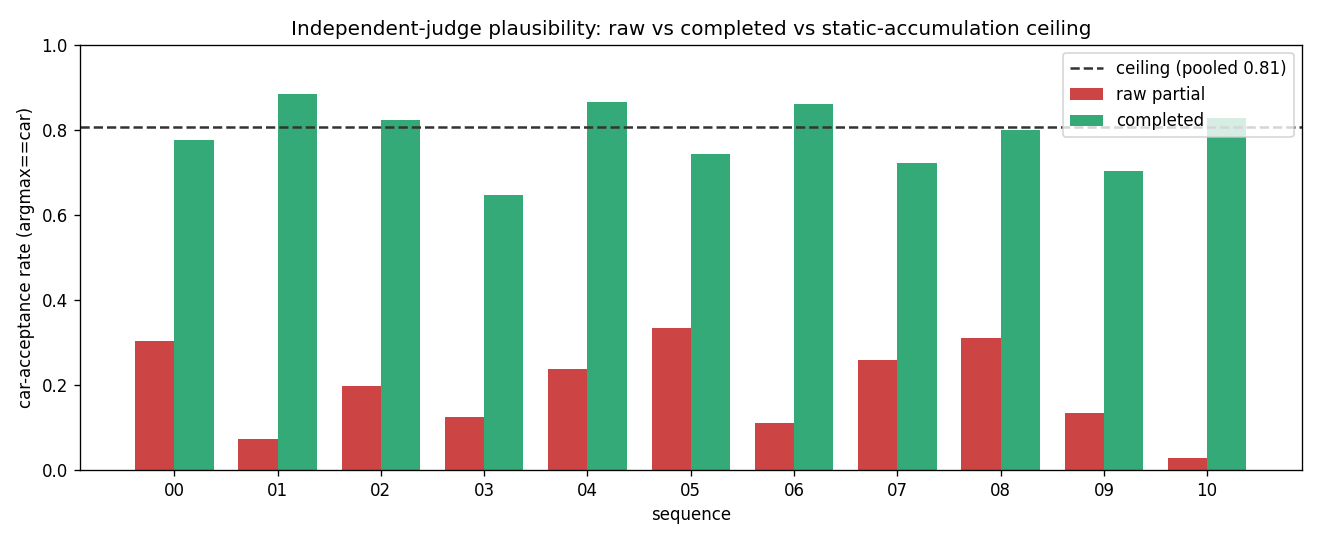
\includegraphics[width=\linewidth]{plausibility_acceptance.png}
  \caption[Plausibility by sequence]{Car-acceptance of the independent judge, per sequence:
    raw single-frame partial (red) against the PCN completion (green), with the pooled
    static-accumulation ceiling (dashed). Completion lifts acceptance several-fold on every
    one of the eleven labelled sequences and sits at or near the ceiling throughout;
    sequence~08, on which the completion constants were tuned, is not an outlier, so the
    result is not an artefact of tuning.}
  \label{fig:plausibility}
\end{figure}

\paragraph{The gain holds on every sequence:} The completion constants were developed on
sequence~08, so a fair test is whether the plausibility gain appears on sequences that took
no part in that development. Figure~\ref{fig:plausibility} and Table~\ref{tab:plausibility-seq}
show it does: completed acceptance ranges from \num{0.646} to \num{0.885} across the eleven
sequences, several times the raw-partial rate on each, and sequence~08 (\num{0.311}
$\to$~\num{0.799}) is unremarkable among them. The completion network was trained only on
synthetic data and never saw any real sequence, so this consistency is a direct
generalisation result.

\begin{table}[H]
  \centering
  \caption[Plausibility acceptance by sequence]{Car-acceptance by sequence, raw partial vs.\
    completed, over all eleven labelled sequences ($N$ = paired tracks per sequence).}
  \label{tab:plausibility-seq}
  \small
  \setlength{\tabcolsep}{4.5pt}
  \begin{tabular}{lccccccccccc}
    \toprule
    Seq & 00 & 01 & 02 & 03 & 04 & 05 & 06 & 07 & 08 & 09 & 10 \\
    \midrule
    $N$ & 926 & 96 & 329 & 48 & 59 & 258 & 164 & 213 & 518 & 141 & 70 \\
    Raw & 0.30 & 0.07 & 0.20 & 0.13 & 0.24 & 0.33 & 0.11 & 0.26 & 0.31 & 0.13 & 0.03 \\
    Compl.\ & 0.78 & 0.89 & 0.82 & 0.65 & 0.86 & 0.74 & 0.86 & 0.72 & 0.80 & 0.70 & 0.83 \\
    \bottomrule
  \end{tabular}
\end{table}

\paragraph{Moving cars complete as plausibly as static ones:}
\label{sec:results-movers}
Because completion runs on a single reference frame's cluster rather than on accumulated
points, there is no motion smear in its input, so motion is not expected to matter. Labelling
each track static or moving by the net displacement of its centroid confirms it: the moving
subset ($N=\num{602}$) reaches completed acceptance \num{0.837} and car-probability
\num{0.801}, if anything slightly above the static subset. The static-only ceiling comparison
above therefore does not hide a mover failure mode.

\paragraph{Heading ambiguity is not a confound:} The harmonisation fixes each cloud's up axis
and length axis but leaves front-versus-back ambiguous (the footprint fit does not resolve
heading sign). Re-scoring every completed cloud with an added \SI{180}{\degree} heading flip
changes acceptance by only \num{0.009}, so the residual heading ambiguity does not affect the
result.

\subsection{Reference-Free Fidelity and Its Caveat}
\label{sec:results-fidelity}

The field's established reference-free metrics score a completion by how closely it reproduces
its own observed input: the unidirectional Chamfer and Hausdorff distances (UCD, UHD;
Section~\ref{sec:th-distances}), applied to real KITTI cars by Chen et
al.~\cite{chen2020unpaired} and P2C~\cite{cui2023p2c}. Computed on the seq-08 cars
(input\,$\to$\,cloud direction, per-car medians), they behave exactly as their definition
dictates (Table~\ref{tab:fidelity}): the raw partial is a trivial optimum at \num{0}, because
it is its own input, while the completion is scored worst, penalised for every point it
adds beyond the observed side.

\begin{table}[H]
  \centering
  \caption[Reference-free fidelity metrics]{Reference-free fidelity on seq-08 cars
    (\num{39} cars, per-car medians, input\,$\to$\,cloud direction; lower is ``better'' in the
    sense of reproducing the observed input). The raw partial is the trivial optimum and the
    completion scores worst, the metrics reward under-completion, which is why they cannot
    on their own credit a completion and why the plausibility signal above is the load-bearing
    real-data evidence.}
  \label{tab:fidelity}
  \begin{tabular}{lccc}
    \toprule
    Cloud & UCD (m) $\downarrow$ & UHD$_{\max}$ (m) $\downarrow$ & UHD$_{p95}$ (m) $\downarrow$ \\
    \midrule
    Raw partial        & 0.000 & 0.000 & 0.000 \\
    Mirrored           & 0.000 & 0.000 & 0.000 \\
    \textbf{Completed} & 0.090 & 0.286 & 0.183 \\
    \bottomrule
  \end{tabular}
\end{table}

This is not a negative result about the completion; it is a property of the metrics. An
input-fidelity measure is minimised by the cloud that adds nothing, so it structurally cannot
reward recovering unobserved surface. This is precisely why the unpaired-completion literature
pairs UCD/UHD with a separate plausibility term~\cite{chen2020unpaired}, and why this thesis
reports fidelity honestly here but rests its favorable real-data claim on the plausibility of
Section~\ref{sec:results-plausibility}.

\subsection{Scope of the Completion Claim}
\label{sec:results-completion-scope}

The completion evidence is deliberately scoped. The network works in distribution on
synthetic shapes (Chamfer \SI{0.16}{\meter}, F@\SI{0.1}{\meter} \num{0.76}), but synthetic
performance is not a real-data claim. On real LiDAR the favorable evidence is the
independent-classifier plausibility: completion lifts car-acceptance from \num{0.253} to
\num{0.785}, reaching the static-accumulation shape ceiling, consistently across all eleven
sequences and for moving as well as static cars. The reference-free fidelity metrics do not
credit the completion, and are reported as such rather than omitted. The claim the thesis
makes is therefore this and no more: on real automotive LiDAR, learned completion produces
shapes an independent classifier accepts as cars far more often than the raw partials, and as
often as dense correctly-shaped references, while established fidelity metrics, which reward
reproducing the input, do not credit it. A remaining limitation of the production path is the
per-car length estimate's fixed-prior fallback on tracks with fewer than five gate-passed
frames (Section~\ref{sec:completion-length}); on the seq-08 output this fallback is used by a
non-trivial fraction of tracks and is revisited in the discussion.

\section{Ablation Studies}
\label{sec:results-ablations}

This section decomposes both halves of the system into the contribution of each
component, in two groups: detection ablations
(Section~\ref{sec:abl-detection}) and completion ablations
(Section~\ref{sec:abl-completion}). Every ablation is produced under the frozen
protocol of Section~\ref{sec:eval-protocol} unless a deviation is stated explicitly.

\subsection{Detection Ablations}
\label{sec:abl-detection}

\paragraph{Stage decomposition (classifier and track filter):}
\label{sec:ablation-stage}

Table~\ref{tab:ablation-stage} isolates the two filtering stages that sit on top
of geometric clustering. The geometric-only row uses clustering plus the
geometric size/shape filters with no learned classifier and no
track filter (like-for-like under the promoted
configuration); the full row is the headline.

\begin{table}[H]
  \centering
  \caption[Stage ablation on seq~08]{Stage ablation on the full sequence~08 (frozen configuration). Rows
    add one filtering stage at a time on top of geometric clustering. The
    per-frame classifier is the precision mechanism (it removes $\sim$\num{104000}
    junk clusters) but is conservative on borderline cars (recall drops); the
    offline track filter then recovers recall by temporal voting while raising
    precision further. Mean IoU is over matched detections only. Geometric-only
    and the middle row are per-frame (no track filter); the full row uses the
    offline track filter.}
  \label{tab:ablation-stage}
  \setlength{\tabcolsep}{5pt}
  \begin{tabular}{lccccc}
    \toprule
    Configuration & Precision & Recall & $F_1$ & Mean IoU & TP / FP / FN \\
    \midrule
    Geometric only                & 0.199 & 0.773 & 0.316 & 0.907 & \num{27002} / \num{108831} / \num{7920} \\
    \;+\,classifier              & 0.846 & 0.676 & 0.751 & 0.922 & \num{23600} / \num{4303} / \num{11322} \\
    \;+\,classifier, track filter & 0.911 & 0.732 & 0.812 & 0.913 & \num{25568} / \num{2513} / \num{9354} \\
    \bottomrule
  \end{tabular}
\end{table}

The decomposition tells a two-step story. The classifier
is the precision mechanism: geometric clustering under the promoted coarse-voxel
setting emits many mostly-junk clusters (precision \num{0.199}), and the per-frame
classifier removes about \num{104000} of them across the sequence
(FP \num{108831}~$\rightarrow$~\num{4303}), lifting precision from \num{0.199} to
\num{0.846}. It pays for this with recall, being conservative, it discards
borderline true clusters too, so recall falls from \num{0.773} to \num{0.676}.
The track filter then recovers that recall while improving precision
again: linking detections across frames and accepting only consistent tracks
lifts precision to \num{0.911} and recall to \num{0.732} (TP
\num{23600}~$\rightarrow$~\num{25568}), because a car seen across many frames is
kept even where a single frame classified it as unknown, while transient
false positives fail the track-length test. The net of both stages is still a
recall trade, geometric-only recall (\num{0.773}) exceeds the full-pipeline
recall (\num{0.732}), roughly \num{1400} true positives forgone for the
$\sim$\num{106000}-false-positive removal, but that trade runs through a
recall dip and a partial recovery, not a simple monotone loss. We report it
rather than hiding it: the system is deliberately tuned for precision, and the
recall it forgoes here is small next to the recall it never had (Section~\ref{sec:recall-analysis}). The
pre-promotion geometric-only figure ($F_1$~\num{0.305}) is
superseded by this like-for-like \num{0.316} and kept only as a historical
record.

\paragraph{Redundancy of synthetic pretraining (Stage~A ablation):}
\label{sec:ablation-stagea}

The classifier ships as a binary car/not-car network trained from scratch
on mined real clusters (Stage~B). A natural alternative is a two-stage
recipe in which a synthetic-ShapeNet Stage~A pretraining seeds Stage~B; we tested
whether that pretraining is necessary and found it is not, a negative result we
report as a finding, because it changes the recommended recipe.

At the classifier level, on the sequence~08 validation clusters, the from-scratch
network matches the pretrained one: macro $F_1$ \num{0.9285} from scratch versus
\num{0.9225} pretrained (the two are within run-to-run noise, with
scratch marginally ahead). At the pipeline level the two checkpoints are
identical in $F_1$ to three decimals on the full sequence~08. We therefore
drop Stage~A from the production pipeline and keep it as ablation material.

The reason the synthetic prior is redundant, and cannot simply be added for
safety, is a total, symmetric domain gap between synthetic and real point
clusters. Table~\ref{tab:cross-domain} gives the cross-domain
transfer matrix: a model trained on one domain and evaluated on the other scores
a car-class $F_1$ of \num{0.000} in both off-diagonal directions, and
fine-tuning on real data erases whatever the synthetic pretraining had learned.
Given \num{420000} real training clusters, the real data does essentially all the
work; the synthetic prior neither helps nor, once fine-tuned, survives.

\begin{table}[H]
  \centering
  \caption[Cross-domain classifier transfer]{Cross-domain classifier transfer (car-class $F_1$). Each
    model is trained on one domain and evaluated on the other's validation set;
    diagonal cells (italic) are in-domain, for scale. Both off-diagonal cells
    collapse to \num{0.000}, against strong in-domain performance
    (\num{0.999}, \num{0.885}), so synthetic and real clusters are mutually
    out-of-distribution and synthetic pretraining transfers nothing to real
    inference.}
  \label{tab:cross-domain}
  \begin{tabular}{lcc}
    \toprule
    & \multicolumn{2}{c}{Evaluated on} \\
    \cmidrule(lr){2-3}
    Trained on & Synthetic & Real \\
    \midrule
    Synthetic (Stage~A) & 0.999 & 0.000 \\
    Real (Stage~B)      & 0.000        & 0.885 \\
    \bottomrule
  \end{tabular}
\end{table}

\paragraph{Cost and benefit of HDBSCAN clustering:}
\label{sec:ablation-clustering}

The clustering stage is HDBSCAN. Because it is by far the most expensive stage
(Section~\ref{sec:results-runtime}), we benchmarked it against two cheaper
density/connectivity clusterers, DBSCAN and Euclidean-tolerance clustering,
at the same voxel resolution and under an identical pipeline
(Table~\ref{tab:clustering}). Deviation: this benchmark is
per-frame with the track filter off, because it strides across the
sequence and the tracker requires contiguous frames; the numbers are therefore
comparable to each other but not to the track-filtered headline.

\begin{table}[H]
  \centering
  \caption[Clustering-method benchmark]{Clustering-method benchmark at fixed voxel resolution
    ($\SI{0.10}{\metre}$), identical pipeline, per-frame / track-filter-off. HDBSCAN wins $F_1$ on both sequences, entirely through
    recall; precision is essentially method-independent. The alternatives are
    4--6$\times$ faster. Mean IoU is over matched detections; the timing column is
    the mean per-frame clustering time.}
  \label{tab:clustering}
  \begin{tabular}{llccccc}
    \toprule
    Seq & Method & Precision & Recall & $F_1$ & Mean IoU & Clustering (mean ms) \\
    \midrule
    \multirow{3}{*}{00}
      & HDBSCAN   & 0.972 & \textbf{0.731} & \textbf{0.835} & 0.968 & 306 \\
      & DBSCAN    & 0.975 & 0.637 & 0.771 & 0.964 & 54 \\
      & Euclidean & 0.979 & 0.636 & 0.771 & 0.982 & 76 \\
    \midrule
    \multirow{3}{*}{08}
      & HDBSCAN   & 0.840 & \textbf{0.671} & \textbf{0.746} & 0.923 & 320 \\
      & DBSCAN    & 0.870 & 0.565 & 0.685 & 0.927 & 57 \\
      & Euclidean & 0.869 & 0.576 & 0.693 & 0.950 & 75 \\
    \bottomrule
  \end{tabular}
\end{table}

The gap is entirely a recall gap, precision is within \num{0.030} across all
methods on either sequence, while HDBSCAN's recall exceeds the alternatives by
\numrange{9}{11} points. An $\varepsilon$-sweep confirms no fixed radius closes
it: the best fixed-radius setting (Euclidean at $\varepsilon=\SI{0.4}{\metre}$)
reaches $F_1$ \num{0.800} on sequence~00, still short of HDBSCAN's \num{0.835}.
HDBSCAN's variable-density criterion recovers cars that a single radius cannot,
which is exactly the recall margin that matters here. We therefore
adopt nothing from the benchmark and keep HDBSCAN in production, paying
its runtime cost knowingly; DBSCAN and Euclidean remain available as
command-line options for reproduction.

\subsection{Completion Ablations}
\label{sec:abl-completion}

These ablations isolate the effect of each completion-pipeline choice; they vary one
component of the completion path (Section~\ref{ch:completion-method}) and re-run the
completion, with the completion network itself unchanged.

\paragraph{Inference normalisation:} PCN is trained in a canonical car frame, so a real
partial must be mapped into that frame before completion
(Section~\ref{sec:completion-normalisation}). The importance of this step is the
semantics-map lesson of Section~\ref{sec:completion-inferencebug} made concrete: with the
canonical-frame normalisation, the completed clouds are recognisably car-shaped and
correctly oriented; with a naive alternative, aligning the partial to a 3D PCA frame and
normalising by its own centroid and radius, the same checkpoint produces mis-oriented,
mis-scaled blobs, because the 3D PCA picks an arbitrary principal axis rather than gravity.
The blob-versus-car difference is entirely a normalisation effect, not a network one, since
the checkpoint is identical.

\paragraph{Input-quality gate:} The L-shape gate decides whether a detected car reaches
completion as a clean single-object cluster (Section~\ref{sec:completion-lshape}). It
rejects HDBSCAN fragments and merges, which would otherwise feed the completion network an
input that is not one whole car and complete into an implausible shape. On seq~08 every
implausible completion originated from a fragment or merge input, so the gate is what keeps
the production completions clean; it carries a measured cost, dropping a fraction of
otherwise-usable cars as false rejections, which is stated as a limitation rather than
hidden.

\paragraph{Length geometry:} A partial truncated at the occluded far end completes short,
so the completion tends to under-extend length (Section~\ref{sec:completion-length}). The
production path corrects this with a per-car length estimate rather than a single fixed
prior, because a population-median prior over-extends genuinely compact cars while
under-extending long ones. The per-car estimate is the frozen production choice; a residual
far-end under-extension on the longest cars remains, characterised rather than eliminated,
and is carried to the discussion.

\paragraph{Completion architecture (PCN vs.\ PoinTr):} Swapping the completion network
holds the rest of the pipeline fixed. On held-out synthetic cars PoinTr's edge over PCN is
small (Chamfer \SI{0.161}{}$\to$\SI{0.153}{\meter}), a difference too small to justify the
heavier model, and the residual real-data gap is a centroid-estimation limit that is
architecture-independent. PCN is therefore kept off the shelf; the completion result is set
by input quality and geometry, not by the choice of network.

\section{Result Analysis and Error Analysis}
\label{sec:recall-analysis}

The detection operating point above established two facts: the pipeline is
precision-saturated (false positives are low and flat, about \num{0.6} per frame),
and it is recall-limited, missing roughly one car in four
($R=\num{0.732}$ on sequence~08). This section explains why the recall is
limited, and it also underpins the completion results reported earlier
(Section~\ref{sec:results-completion}): the same clustering step that caps recall
is the one that decides whether a detected car reaches completion as a clean
single-object cluster. We show that the shortfall is
a clustering failure rather than a classification failure
(Section~\ref{sec:recall-diagnosis}), root-cause it to HDBSCAN splitting large,
close cars into fragments (Section~\ref{sec:split-analysis}), report a search of
repair strategies that all fail to generalise (Section~\ref{sec:repairs}), and
describe the one intervention that did help, coarsening the clustering
resolution, which forces a correction of an earlier, overstated ``hard
ceiling'' claim (Section~\ref{sec:resolution-fix}). The negative results are
reported as findings, not apologised for: mapping which repairs fail, and why, is
itself a finding worth reporting, and it is what justifies the residual limitation carried to
Chapter~\ref{ch:conclusion}. Unless stated otherwise, the recall denominator
throughout is the one defined in Section~\ref{sec:eval-protocol}, ground-truth
car instances with at least \num{10} points surviving preprocessing.

\subsection{The Shortfall as a Clustering Failure}
\label{sec:recall-diagnosis}

The recall ceiling is upstream of the learned classifier. The stage decomposition
of Section~\ref{sec:results-ablations} makes this direct: geometric clustering with the
size/shape filters but no learned classifier and no track filter
already reaches recall \num{0.773}, which is higher than the full pipeline's
\num{0.732}. Every learned stage that follows can only hold or reduce that recall:
the classifier discards clusters, and the centroid tracker only re-labels and
filters clusters that geometric clustering has already produced, it emits a
detection in a frame only where a cluster exists in that frame, and never
interpolates a detection across a gap, so neither stage can invent a detection where clustering
found nothing. Across the full sequence the two stages together trade roughly
\num{1400} true positives (\num{27002} geometric-only versus \num{25568} full) for the removal of $\sim$\num{106000} false positives; this is a
distinct trade from the $+\num{756}$ true positives that the resolution change of
Section~\ref{sec:resolution-fix} later recovers. Whatever caps recall is therefore
already present in the clusters that geometric clustering produces, before the
classifier sees them.

The geometric filters are not the cap either. Ablation of the
size/shape gates across the full sequence~08 shows that of the
\num{903901} HDBSCAN clusters, \num{127654} (\SI{14.1}{\percent})
pass the filters, and \num{27718} of the rejected clusters overlap a ground-truth
car, dominated by \texttt{min\_volume} (\SI{73.9}{\percent} of the GT-matching
rejections) and \texttt{min\_points} (\SI{12.7}{\percent}). The dominant gates are
\texttt{min\_volume} and \texttt{min\_points}, the two that reject small
clusters. This is consistent with the rejected clusters being the smaller
sub-fragments of cars that HDBSCAN has already split (the dominant fragment passing
while the splinters fail the size gates), which the split analysis of
Section~\ref{sec:split-analysis} then confirms is the prevailing failure mode. We
state this as an inference rather than a direct measurement: the ablation records
only that a rejected cluster overlaps some ground-truth car,
not whether that same car also retains a
surviving cluster, so it establishes that the rejections are dominated by small
fragments, not that every one belongs to an otherwise-detected car. Either way the
diagnosis points one stage further upstream, at the clustering itself.

\subsection{Root Cause: HDBSCAN Fragmentation of Large, Close Cars}
\label{sec:split-analysis}

To quantify how clustering caps recall we measured, for every eligible ground-truth
car, how its points distribute across HDBSCAN clusters. Each car is
assigned to exactly one of four states that partition the population: ok (one
dominant cluster, under \SI{30}{\percent} noise), split (points spread over
two or more clusters), noisy (one cluster but at or above \SI{30}{\percent}
noise), or all-noise. A separate, cross-cutting flag marks merged cars
(a car whose dominant cluster is shared with another car); a merged car still has a
dominant cluster, so it is not a fifth partition class and is reported below
as a memo count rather than a table row that would be summed.
Table~\ref{tab:split} gives the result on the full sequence.

\begin{table}[H]
  \centering
  \caption[Ground-truth cars across HDBSCAN clusters]{Distribution of ground-truth cars across HDBSCAN clusters
    (full sequence~08, \num{34057} eligible cars, pre-promotion
    \SI{0.05}{\metre} clustering configuration). The four states partition the
    population and sum to the denominator; split is the dominant failure mode and
    merging (the cross-cutting memo row, not summed) is negligible. Split cars are
    uneven, the largest fragment holds a median \num{0.79} of the points, but a
    large point-fraction does not guarantee a match (see text).}
  \label{tab:split}
  \begin{tabular}{lcc}
    \toprule
    & \multicolumn{2}{c}{Seq 08 (\num{34057} cars)} \\
    \cmidrule(lr){2-3}
    Status & Count & \% \\
    \midrule
    ok (single dominant cluster) & 18769 & 55.1 \\
    split (2+ clusters)          & 15245 & 44.8 \\
    noisy / all-noise            & 43    & 0.1  \\
    \midrule
    partition total              & 34057 & 100  \\
    \addlinespace
    merged (cross-cutting) & 56 & 0.2 \\
    \bottomrule
  \end{tabular}
\end{table}

Three things follow. First, splitting, not merging, is the failure mode:
\SI{44.8}{\percent} of cars split, while merging is \SI{0.2}{\percent}. The pipeline
almost never fuses two cars into one detection; it
repeatedly breaks one car into several. Second, the split is worst where
cars are largest and nearest: the split rate falls monotonically with range, at the
adopted \SI{0.10}{\metre} resolution \SI{53.5}{\percent} at \SIrange{0}{10}{\metre},
\SI{40.2}{\percent} at \SIrange{10}{20}{\metre}, \SI{22.3}{\percent} at
\SIrange{20}{40}{\metre}, and \SI{3.5}{\percent} past \SI{40}{\metre}. Large, close
cars return many points, and
HDBSCAN finds internal density variations within that dense return, the roof line
against the body, the near side against the far side, and cuts the car along
them. This is the mechanism behind the counter-intuitive near-range recall dip
reported in Section~\ref{sec:results-distance}: the nearest bin has lower recall than
the \SIrange{10}{20}{\metre} bin despite carrying far more points, because a close
car dissolves into fragments that no longer match the whole instance. Third,
the cleanly-clustered fraction is a floor on recall, and splitting is the dominant
loss above it. The fraction of cars that form one dominant cluster
(\SI{55.1}{\percent} at the pre-promotion configuration) sits below the recall the
pipeline achieves there (\num{0.710}): the pipeline recovers essentially every
cleanly-clustered car and, in addition, a portion of the split cars whose dominant
fragment survives matching and filtering, so recall clears the clean fraction rather
than sitting at it. Splitting nonetheless remains the dominant loss mode,
\SI{44.8}{\percent} of cars split and the majority of those are still lost, because
a large dominant point-fraction (median \num{0.79}) does not translate into a match
when the fragment must also clear the size filters. This predicts the resolution fix
of Section~\ref{sec:resolution-fix}: coarsening the voxel converts split cars into
clean ones, which should lift recall by raising the clean fraction and shrinking the
reliance on recovering split fragments, and it does, raising the clean fraction from
\SI{55.1}{\percent} to \SI{66.0}{\percent} and recall from \num{0.710} to
\num{0.732}, and narrowing the gap between clean fraction and recall from \num{15.9}
to \num{7.2} points.

Figure~\ref{fig:failure-zooms} shows the mechanism directly on three sequence~08
frames. Missed cars (orange) appear as broken rows of points close to the ego
vehicle, each row too small on its own to survive the size filters, while cleaner
mid- and far-range cars (green) are detected as single clusters.

\begin{figure}[htbp]
  \centering
  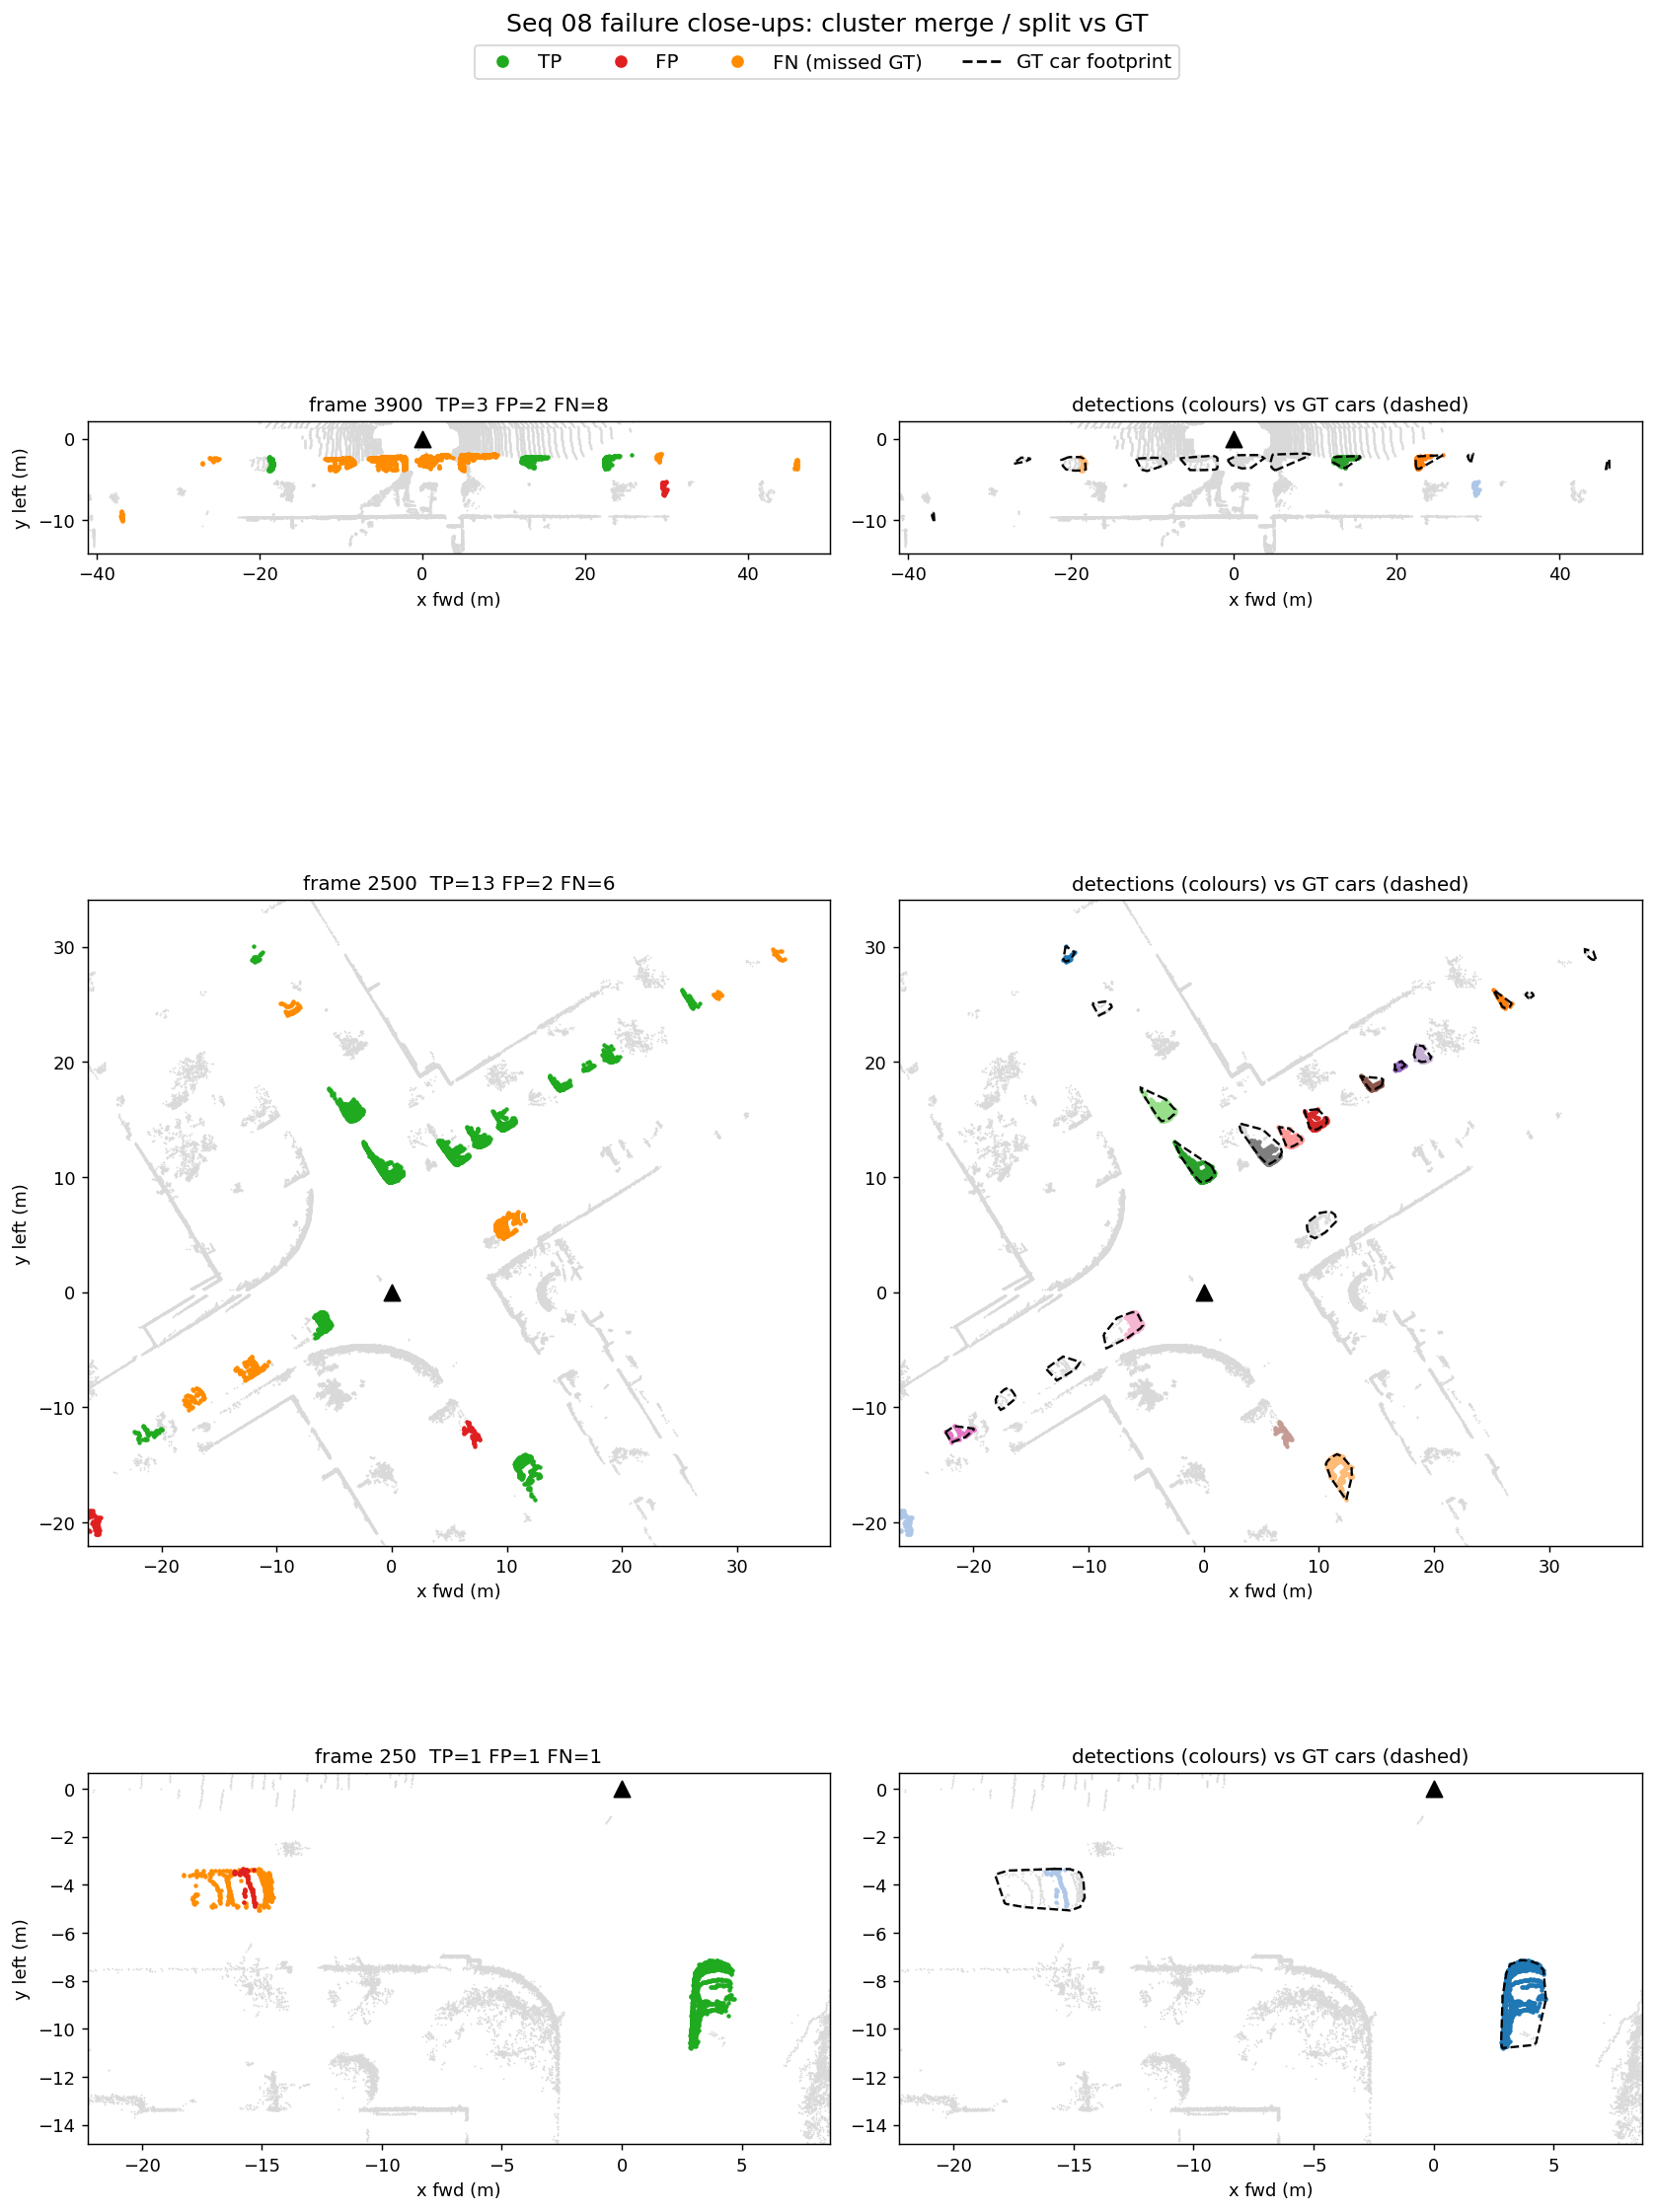
\includegraphics[width=\linewidth]{seq08_failure_zooms.png}
  \caption[Detection failure close-ups on seq~08]{Failure close-ups on sequence~08 (true positives green, false positives
    red, missed ground-truth cars orange; dashed outlines are ground-truth car
    footprints). Near-ego missed cars are fragmented into several small point groups
    rather than one cluster, matching the split mechanism of
    Table~\ref{tab:split}. Although the panel title mentions both merge and split,
    merging is measured at $\leq\!\SI{0.5}{\percent}$ (Table~\ref{tab:split}), so the
    misses shown are fragmentation, not fusion of neighbouring cars.}
  \label{fig:failure-zooms}
\end{figure}

\subsection{Limits of the Repair Strategies}
\label{sec:repairs}

Given that splitting caps recall, the obvious responses fall into two families:
change how clusters form (a larger minimum cluster size, a different
clusterer, distance-adaptive parameters, or pre-clustering point accumulation) or
reassemble fragments after HDBSCAN has split them. We tried six in total;
Table~\ref{tab:strategies} collects the four with a reproducible quantitative
outcome, and two further strategies (temporal accumulation and threshold lowering)
are discussed in prose below. All were evaluated against the same pre-promotion
sequence-00 baseline (full pipeline, classifier and track filter on;
$F_1=\num{0.844}$), and the load-bearing ones were re-checked on the held-out
sequence~08.

\begin{table}[H]
  \centering
  \caption[Recall-repair strategies]{Recall-repair strategies against the pre-promotion baseline (full
    pipeline, classifier and track filter on, on a sequence-00 sample; held-out
    sequence-08 $F_1$ where measured). This is an exploratory pre-promotion repair
    search: it predates the coarse-voxel configuration of
    Section~\ref{sec:resolution-fix} (which is why the baseline here is
    $F_1=\num{0.844}$, not the promoted headline), and it is reported to establish the
    mechanism by which each strategy fails rather than as headline metrics. Every
    strategy either loses $F_1$ outright or fails to hold its sequence-00 gain on the
    held-out sequence; the adopted resolution and its full-sequence numbers are given in
    Section~\ref{sec:resolution-fix}. Sources in the ``Src'' column are
    finding numbers. Two further strategies, temporal point accumulation and
    lowering the size thresholds, are discussed in the text but omitted here:
    temporal accumulation is single-sourced to a reverted feature in the session
    log (not reproducible under the research freeze), and threshold lowering
    produced no change in true positives; both belong in prose rather than the main
    results table.}
  \label{tab:strategies}
  \setlength{\tabcolsep}{4pt}
  \begin{tabular}{lcccc}
    \toprule
    Strategy & Seq 00 $P$ & Seq 00 $R$ & Seq 00 $F_1$ & Seq 08 $F_1$ \\
    \midrule
    Baseline (HDBSCAN, MCS \num{10}) & 0.984 & 0.739 & \textbf{0.844} & \textbf{0.829} \\
    BEV clustering (res \SI{0.30}{\metre})   & 0.993 & 0.640 & 0.779 &, \\
    Higher MCS \num{20}                       & 0.976 & 0.755 & 0.852 & 0.801 \\
    Fragment merge (\SI{1.5}{\metre}, \num{30}\,pt) & 0.931 & 0.755 & 0.834 & 0.815 \\
    Adaptive HDBSCAN (\num{30}/\num{15}/\num{10}) & 0.935 & 0.748 & 0.831 &, \\
    \bottomrule
  \end{tabular}
\end{table}

Each strategy fails for a structural reason, and the reasons are consistent with the
diagnosis of Section~\ref{sec:split-analysis}:

\begin{itemize}
  \item Higher minimum cluster size (MCS \num{20}) is the most instructive.
    It is the only variant to improve $F_1$ on sequence~00
    (\num{0.844}~$\rightarrow$~\num{0.852}), by discouraging the small splinter
    clusters. But it does not generalise: on the held-out sequence~08 it drops to
    $F_1$~\num{0.801}, below the \num{0.829} baseline, because a larger
    minimum also erases genuinely sparse distant cars. The sequence-00 gain was
    over-fitting.
  \item Post-clustering fragment merge (join clusters within
    \SI{1.5}{\metre}) raises sequence-00 recall to \num{0.755} but loses precision
    (\num{0.984}~$\rightarrow$~\num{0.931}), because the same proximity rule also
    fuses nearby non-car structure (walls, poles) into oversized clusters. On
    held-out data the precision loss cancels the recall gain
    ($F_1$~\num{0.815}~$<$~\num{0.829}).
  \item Distance-adaptive HDBSCAN (a larger minimum cluster size near the
    ego, smaller far away) introduces boundary artefacts at the ring transitions and
    is worse than the global setting.
  \item Bird's-eye-view clustering, a cheaper
    connected-component alternative, collapses recall to \num{0.640}: projecting to
    two dimensions merges objects that overlap in the ground plane but are separated
    in height, and morphological cleanup destroys sparse distant clusters.
  \item Temporal aggregation, accumulating object points over three
    consecutive frames before clustering, to densify sparse cars, collapses the
    pipeline ($F_1$~\num{0.073}, recall \num{0.039}).\footnote{Source:
    \texttt{docs/session\_history.md} (2026-06 exploratory session). The
    \texttt{temporal\_window} feature was implemented and then fully reverted, so
    this result is on the pre-promotion baseline and was not re-run under the
    research freeze; it is reported here in prose, not in Table~\ref{tab:strategies},
    for that reason, and its value is the mechanism below rather than the exact
    figure.} Accumulating points does not densify
    the existing clusters; it reshapes the clustering landscape entirely
    (about \num{134000} accumulated points yield \num{645}+ clusters versus
    $\sim$\num{240} single-frame, of which fewer pass the geometric filters,
    \num{17} versus \num{34}).
  \item Lowering the cluster-size thresholds to admit sparser groups
    produced no change in true positives at all: the binding constraint is cluster
    quality, not the count threshold, so relaxing the threshold merely admits more
    noise (\texttt{docs/session\_history.md}).
\end{itemize}

The failure modes are strategy-specific, over-fitting, precision loss, ring
artefacts, projection ambiguity, a reshaped clustering landscape, but they share
a limit. The two strategies that reassemble after the split (fragment merge, and to
a lesser extent the proximity-based part of the adaptive scheme) run into the fact
that density-based clustering has no notion of objectness: once a dense car is
partitioned along an internal density gap, no proximity- or size-based rule can
reliably tell ``rejoin these two fragments of one car'' apart from ``do not join
these two adjacent cars.'' The strategies that instead change how clusters
form, a larger minimum size, a different clusterer, per-ring parameters,
pre-clustering accumulation, avoid the reassembly trap but hit the same wall from
the other side: any single global density criterion that is loose enough to keep a
split car whole is also loose enough to fuse a close pair, so a sequence-00 gain
becomes a held-out loss. The one lever that helped, changing the clustering
resolution (Section~\ref{sec:resolution-fix}), is also a formation change; it
works not by escaping this limit but by happening to sit at a resolution that closes
intra-car gaps before it starts closing inter-car ones. This is why the earlier
project conclusion, that recall was fixed at a hard ceiling of about \num{0.74}
, was reasonable given only the evidence
in Table~\ref{tab:strategies}, and also, as the next section shows, wrong: it read a
limit on these repairs as a limit on the approach.

\subsection{Clustering Resolution and the Corrected Ceiling}
\label{sec:resolution-fix}

The intervention that helped was not a repair at all but a change to the clustering
resolution: re-voxelising the object cloud to a \SI{0.10}{\metre} grid
before running HDBSCAN, rather than clustering the full-resolution
\SI{0.05}{\metre} cloud (adopted in the runtime optimisation of
Section~\ref{sec:results-runtime}). A coarser grid closes the small intra-car density gaps that HDBSCAN was
cutting along, so fewer splits form in the first place. It is a formation change like
the failed ones in Section~\ref{sec:repairs}, but it lands on the favourable side of
the trade described there, coarse enough to close intra-car gaps, still fine
enough not to fuse neighbouring cars.

\begin{table}[H]
  \centering
  \caption[Effect of coarsening the clustering voxel]{Effect of coarsening the clustering voxel from \SI{0.05}{\metre} to
    \SI{0.10}{\metre} on the split rate (full sequence~08, \num{34057}
    ground-truth cars). Coarsening removes splits but is not free: it also
    fuses some neighbouring cars, so the merge count rises even as the split rate falls.}
  \label{tab:splitrate}
  \begin{tabular}{lcc}
    \toprule
    & Full-res (\SI{0.05}{\metre}) & Coarse (\SI{0.10}{\metre}) \\
    \midrule
    clustered ``ok''            & 18769 (55.1\%) & 22487 (66.0\%) \\
    split                        & 15245 (44.8\%) & 11480 (33.7\%) \\
    merged (cross-cutting)       & 56 (0.2\%)     & 284 (0.8\%)    \\
    mean clusters per split car  & 4.7            & 3.0 \\
    \bottomrule
  \end{tabular}
\end{table}

Table~\ref{tab:splitrate} shows the split rate falling by \num{11.1} points
(\SI{44.8}{\percent}~$\rightarrow$~\SI{33.7}{\percent}). This is a trade, not a
free lunch: the coarser grid also fuses some adjacent cars, so the merged count
rises from \num{56} to \num{284} (\SI{0.2}{\percent}~$\rightarrow$~\SI{0.8}{\percent}).
The gain still dominates, roughly \num{3700} cars move from split to clean while
about \num{230} newly merge, but the merge cost is real and bounds how far
coarsening can be pushed.
At the pipeline level, on the full sequence~08, this lifts recall from \num{0.710} to
\num{0.732} ($+\num{756}$ true positives) with precision essentially unchanged
(\num{0.910}~$\rightarrow$~\num{0.911}) and $F_1$ from \num{0.798} to \num{0.812}. The same coarsening also reduces clustering runtime, which is why it
was adopted; its detection benefit is the subject here and its runtime co-benefit is
reported in Section~\ref{sec:results-runtime}.

This result forces a correction to the earlier ceiling claim, which we state plainly
rather than bury. The ``$\sim$\num{0.74}
hard limit'' was partly a resolution artefact, not a fundamental property of
the approach: the strategies of Section~\ref{sec:repairs} genuinely do fail, but none
of them tried this particular resolution setting, and changing it recovered part of
the loss. The standing recommendation is therefore
\texttt{cluster\_voxel\_size}~$=\SI{0.10}{\metre}$ in production, not ``accept
\num{0.74}.''

A smaller structural limit does remain, and it is architectural. Coarsening the voxel
further would eventually start merging adjacent cars, trading the split problem for a
merge problem; and the clustering-method benchmark of Section~\ref{sec:results-ablations}
shows that no fixed-radius density clusterer, at any tested radius, reaches even
HDBSCAN's recall. The ceiling that remains is the one imposed by density-based
clustering having no model of what a car is: it groups points by proximity and
density alone, so it cannot be pushed to the recall of a learned object detector by
tuning. Reaching that level would require replacing the clustering stage with a
learned detector, which is outside the scope of this thesis (Chapter~\ref{ch:conclusion}). The
value of this analysis is to have located the ceiling precisely, it is in
the clustering stage, it is splitting rather than classification or merging, and it
is lower than first claimed, and to have mapped which repairs cannot move it and
which one can.

\subsection{Recall Analysis: Summary}
\label{sec:recall-summary}

The recall shortfall is clustering-bound, not classifier-bound: the classifier and
track filter sit on top of a recall ceiling that geometric clustering already imposes
(Section~\ref{sec:recall-diagnosis}). The dominant mechanism is HDBSCAN splitting
large, close cars into fragments, \SI{33.7}{\percent} of cars at the adopted resolution, worst at
short range, while merging is negligible, and the cleanly-clustered fraction sits
just below the achieved recall, so most split cars are lost
(Section~\ref{sec:split-analysis}). A search of six repair strategies, higher
minimum cluster size, fragment merging, adaptive and BEV clustering, temporal
accumulation, and threshold lowering, all fail to generalise, for a shared reason:
density-based clustering has no notion of objectness, so any criterion loose enough to
keep a split car whole also fuses adjacent cars, and reassembling fragments after the
split faces the same ambiguity (Section~\ref{sec:repairs}). The one effective lever was clustering
resolution: a coarser pre-clustering voxel prevents splits from forming, lifting
recall \num{0.710}~$\rightarrow$~\num{0.732} and correcting the earlier overstated
``hard ceiling'' (Section~\ref{sec:resolution-fix}). The residual limit is
architectural, density clustering has no notion of objectness, and is carried
to the limitations and future-work discussion of Chapter~\ref{ch:conclusion}.



% Chapter-summary section removed to mirror the gospel's lean Ch.4; its results
% recap and limitations are carried in Chapter~\ref{ch:conclusion} (Established
% Results and Their Reach; Limitations and Discussion).

% ===== END inlined ch4_evaluation.tex =====
% ===== BEGIN inlined ch5_discussion_conclusion.tex =====
% Chapter 5 -- Discussion and Conclusion (\input by main.tex): discussion + limitations
% + RQ answers + contributions + future work (conclusion half merged in below,
% formerly sec_9_conclusion.tex). Synthesises the detection and completion results into
% a single statement of what the thesis supports, then states every audit-identified
% limitation BY NAME so the committee cannot surface one the thesis has not already named.
%
% Honesty-phrasing rules applied (personal_agenda P1):
%   - claims matched to evidence tier (measured / inferred / speculative) explicitly
%   - "mean IoU" always qualified as "of matched detections"
%   - recall denominator restated (>=10 surviving points, Sec 4.1) wherever recall is cited
%   - completion claims scoped per the T9c outcome (PARTIALLY HOLDS) and to static cars
%   - negative results (#40/#45 etc.) presented as findings, not apologised for; #37 as a
%     metric-design lesson
%   - every number traces to a finding / artifact (cited Finding~\#NN)
%   - the named limitations are all present: detection selection-exposure
%     (bounded by LOSO cross-validation, Sec 4.1: precision-only, ~2 pts), the
%     completion claim resting on plausibility alone (fidelity is unfavorable; synthetic
%     is not real data), the length-estimate fallback (#41), the SemanticKITTI
%     label-quality assumption, the clustering-objectness ceiling (recall analysis, Ch 4),
%     and the offline-runtime scope
%
% Reframe (2026-09-12): main contribution = the modular detection-and-completion
% framework; second = auto-mined supervision and synthetic completion (SemanticKITTI +
% ShapeNet), requiring zero additional manual annotation. The
% old self-made completion metric and box-reference evaluation are dropped; the favorable
% real-data completion evidence is independent-classifier plausibility (Finding #54).
%
\chapter{Conclusion and Future Work}
\label{ch:conclusion}

The preceding chapters reported results; this one interprets them and closes the
thesis. It first draws the conclusions, answering the two research questions and
restating the contributions (Section~\ref{sec:conclusion-rqs}); then gathers what the
evidence supports and how far each claim reaches, together with every limitation the
work carries, into a single section (Section~\ref{sec:disc-limitations}), the
validity of the evaluation, the scope of the completion claims, the ground-truth
assumptions, and the architectural and operational limits, and finally turns the
most consequential boundaries into future work (Section~\ref{sec:conclusion-future}).
Every weakness named here is measured elsewhere in the document and cross-referenced to
the finding that quantifies it: a limitation the thesis names, quantifies, and bounds is
defended; one a committee surfaces first is not.

\section{Conclusion}
\label{sec:conclusion-rqs}

Chapter~\ref{ch:introduction} posed two research questions, one for each half of the
framework; each is answered by the evaluation of Chapter~\ref{ch:evaluation} and restated
here in the form asked, with its reach discussed in Section~\ref{sec:disc-what-holds}.

\paragraph{RQ1, can a modular pipeline requiring zero additional manual annotation detect
and complete occluded vehicles on real LiDAR?} Yes. The framework detects cars with a chain
of training-free classical stages and two small learned models, the classifier trained on
supervision auto-mined from existing semantic annotations and the completion network on
synthetic shapes,
reaching precision \num{0.888}, recall \num{0.717}, and $F_1$~\num{0.793} pooled under
leave-one-sequence-out cross-validation across all eleven labelled sequences, and completes
each detected car with a PCN network. Every stage is separately inspectable, which is what
lets the recall shortfall be root-caused to a single stage rather than left opaque.

\paragraph{RQ2, does learned completion produce car-plausible shapes on real LiDAR, and
how does it fare on established fidelity metrics?} On real cars an independent shape
classifier, trained on external complete-shape data, accepts the completed clouds as cars far
more often than the raw partials (car-acceptance
\num{0.253}~$\rightarrow$~\num{0.785}, paired McNemar and Wilcoxon $p\approx0$) and about as
often as a dense static-accumulation shape ceiling (\num{0.807}), consistently across all
eleven sequences and for moving as well as static cars, so completion produces genuinely
car-plausible shapes rather than denser blobs. The established reference-free fidelity metrics
(UCD, UHD) do not credit the completion: they reward reproducing the observed input, so the
raw partial is their trivial optimum. The favorable real-data claim therefore rests on
plausibility, with fidelity reported honestly as unfavorable.

\paragraph{Diagnostic findings:}
Two findings emerged along the way (Section~\ref{sec:recall-analysis},
Chapter~\ref{ch:evaluation}): recall is clustering-bound, not classifier-bound, HDBSCAN
splits \SI{33.7}{\percent} of cars and a chain of repair strategies fails to
generalise, and synthetic pretraining is redundant once real clusters are plentiful, the
sim-to-real gap being total and symmetric.

\paragraph{Contributions:}
The thesis makes two contributions. The first, and main, is a modular
detection-and-completion framework for occluded vehicles on real LiDAR: an end-to-end,
separately-inspectable pipeline that integrates established components (RANSAC, HDBSCAN,
PointNet, PCN) into a coherent, reproducible system, evaluated end to end. The second is
auto-mined supervision and synthetic completion, an approach requiring zero additional
manual annotation, built on SemanticKITTI (real scans for detection, mining, and
evaluation) and ShapeNet (synthetic complete shapes for completion training), whose
real-data completion quality is assessed with an independent classifier so that no
self-made reference is involved. Two diagnostic findings sit alongside
them, the clustering-bound recall account and the redundancy of synthetic pretraining,
together with the reproducibility infrastructure and documented negative-result lines.

\section{Limitations and Discussion}
\label{sec:disc-limitations}

\subsection{Established Results and Their Reach}
\label{sec:disc-what-holds}

The framework rests on two halves, each with its own evidence. The detection half is
the broadest result: an interpretable clustering front end, requiring zero additional
manual annotation, reaching
precision \num{0.888}, recall \num{0.717}, $F_1$~\num{0.793} pooled under
leave-one-sequence-out cross-validation across all eleven labelled sequences
(Section~\ref{sec:eval-loso}; \num{0.911}~/~\num{0.732}~/~\num{0.812} at the sequence-08
operating point, mean IoU of matched detections \num{0.913}; recall denominator: car
instances with at least \num{10} points surviving preprocessing,
Section~\ref{sec:eval-protocol}), on modest hardware and without state-of-the-art accuracy,
which the supervised networks of Section~\ref{sec:bg-positioning} reach through dense
per-point supervision, whereas this pipeline requires zero additional manual annotation. Its recall shortfall is root-caused, not mysterious,
HDBSCAN splitting large, close cars into fragments (Section~\ref{sec:recall-analysis}).

The completion half's favorable real-data evidence is the independent-classifier
plausibility (Section~\ref{sec:results-plausibility}): completion lifts car-acceptance from
\num{0.253} on the raw partials to \num{0.785}, reaching the dense static-accumulation shape
ceiling (\num{0.807}), consistently across all eleven sequences and for moving as well as
static cars, with the paired gain significant on McNemar and Wilcoxon tests ($p\approx0$).
This is an established protocol (Chen et al.~\cite{chen2020unpaired}) with an external judge
disjoint from the completion network's training data, so it is not circular. In distribution,
on synthetic shapes with a complete ground truth, the network scores Chamfer \SI{0.16}{\metre}
and F@\SI{0.1}{\metre} \num{0.76}. Against these stands the honest negative: the established
reference-free fidelity metrics (UCD, UHD; Section~\ref{sec:results-fidelity}) reward
reproducing the observed input, so they cannot credit the completion, and the favorable claim
rests on plausibility alone.

These reaches vary. The detection operating point is cross-validated across all eleven
sequences (Section~\ref{sec:eval-loso}), and the plausibility gain likewise appears on every
sequence, so both halves transfer beyond the tuning sequence. The recall diagnosis is an
inductive result from the labelled sequences, mechanistic but not a proven invariant, and the
tuned completion constants (the length prior, the estimate quantile, the geometric
thresholds) are sequence-derived and should be re-checked on a new sensor. For practice, three
readings follow: the interpretable detector, requiring zero additional manual annotation, is
a viable choice where labelling budget or inspectability outweighs peak recall, provided the
domain is dense-scene;
independent-classifier plausibility is a reusable, non-circular way to assess real-LiDAR
completion where no complete ground truth exists; and because input quality, not model choice,
governs whether completion is usable, effort is better spent on segmentation than on swapping
architectures. These reaches are bounded by the limitations set out next.

\subsection{Validity of the Evaluation}
\label{sec:disc-eval-validity}

Detection is cross-validated, and the selection exposure is precision-only. SemanticKITTI
labels only sequences \numrange{00}{10}, so no labelled sequence can be reserved as a
conventional held-out detection test set, and the final classifier was historically selected
on sequence~08; leave-one-sequence-out cross-validation (Section~\ref{sec:eval-loso}) bounds
the exposure, the fold-08 classifier matching its recall (\num{0.736} versus \num{0.732}) and
losing only about two precision points (\num{0.888} versus \num{0.911}), so the selection
touched precision, not the clustering-imposed recall ceiling (\num{0.773}) that accounts for
most missed cars. The completion evaluation is guarded on two fronts. It is
non-circular: the plausibility judge is trained on ModelNet40, a shape repository
disjoint from the ShapeNet cars the completion network learned from, so an accepted car is not
an artefact of shared training data, and the completion network never saw a real LiDAR
sequence. And it generalises: the acceptance gain is not a single held-out replication
but appears on all eleven labelled sequences (Section~\ref{sec:results-plausibility}), with
the tuning sequence~08 unremarkable among them. Its one honest asymmetry is that the favorable
evidence is plausibility alone; the established fidelity metrics do not corroborate it,
because they reward under-completion, and synthetic fidelity is not a real-data claim.

\subsection{Scope of the Completion Claims}
\label{sec:disc-completion-scope}

The completion claim is deliberately bounded. The favorable real-data evidence is a single
established instrument, independent-classifier plausibility, and it measures whether a
completed cloud reads as a car, not metric surface accuracy against a complete shape, which
no real-LiDAR reference can supply. The established reference-free fidelity metrics do not
corroborate it, so the claim rests on plausibility alone and must not be read as a
surface-reconstruction-accuracy claim. Plausibility scores only clean, gate-passed clusters,
and whether a car reaches completion as one is decided upstream by the clustering that caps
recall: the L-shape input gate rejects fragments and merges that would otherwise complete
implausibly (Section~\ref{sec:abl-completion}), whereas swapping PCN for PoinTr changes the
result not at all, so widening completion's reach is a segmentation problem, not a
completion-architecture one.

Within that scope, two residuals bound the completed shape. The per-car length estimate falls
back to the \SI{4.14}{\metre} population prior on tracks with fewer than five gate-passed
frames, a non-trivial fraction of sequence-08 tracks, reintroducing some compact
overshoot there, on the sparsest, most distant cars where it matters least. Even with an
unbiased estimate the completed cloud stays slightly short at the far end by an amount that
scales with car length: a pre-registered fix removed this on normal and long cars but
over-extended compacts, so the compensation is irreducibly length-dependent and the far end
remains the weakest-covered region. Both residuals compound the model's synthetic-only
training, the source of the evaluation's independence, but also a synthetic-to-real gap
(Section~\ref{sec:bg-completion}) behind the residual flatness of the sparsest real
completions.

\subsection{Ground-Truth and Dataset Assumptions}
\label{sec:disc-gt}

Two assumptions underlie the ground truth. Recall is reported against eligible cars, those
with at least \num{10} points surviving preprocessing, which excludes \SI{25.5}{\percent}
of annotated cars too sparse or distant to reach the front end, so recall against all
annotated cars is approximately \num{0.55} against the \num{0.732} eligible figure (both
reported; the two ``$\geq$10-point'' rules are distinct). And all counts and matches assume
SemanticKITTI's labels are correct; we did not audit them, and mislabelled cars would
propagate into the detection metrics and the mined classifier labels. The completion
evaluation avoids a self-made reference entirely: its plausibility judge is scored against
ModelNet40's own labels, and the raw-versus-completed comparison is paired on identical
inputs, so no accumulated pseudo-ground-truth enters the completion claim.

\subsection{Architectural and Operational Limits}
\label{sec:disc-architectural}

The remaining limits are architectural or operational. The recall ceiling is architectural,
not a tuning failure (Section~\ref{sec:recall-analysis}): coarsening the cluster voxel to
\SI{0.10}{\metre} recovered part of the loss (\num{0.710}~$\rightarrow$~\num{0.732}) but
coarsening further fuses adjacent cars, and no fixed-radius density clusterer reaches HDBSCAN's
recall at any tested radius, so the ceiling (\num{0.773} before any learned stage, splitting
\SI{33.7}{\percent} of cars) is the measured price of the interpretable design,
requiring zero additional manual annotation, the thesis exists to evaluate, and lifting it
means a learned detector, a different system. The operational domain is dense scenes: recall falls to
\num{0.336} on the sparse highway sequence~01 against \num{0.758} on dense-urban sequence~00,
mostly because highway cars are distant and recall collapses with range (\num{0.196} beyond
\SI{40}{\metre}) and partly because the front end was tuned on dense data, though the failure
is a conservative miss, not a false alarm (sequence~01 precision \num{0.951}). The system is
offline by design, running at about \SI{623.5}{\milli\second} per frame
(Section~\ref{sec:results-runtime}) with the $\leq\SI{400}{\milli\second}$ target unreachable
through the authorised tiers, and real-time operation is out of scope. Finally, the centroid
tracker feeds the per-car length estimate and drives its fixed-prior fallback but is never
scored as a tracker (no MOTA or IDF1), so its contribution to that fallback is unmeasured.

% Conclusion moved to the top of this chapter (Section~\ref{sec:conclusion-rqs}) to
% mirror the Conclusion-first order; the Established Results discussion is folded into
% Limitations and Discussion above. Honesty-phrasing rules (personal_agenda P1) still
% apply: favorable real-data completion evidence = independent-classifier plausibility
% alone (#54), fidelity unfavorable, movers complete as plausibly as statics, negatives
% as findings.

\section{Future Work}
\label{sec:conclusion-future}

The limitations above named the boundaries of the present results. Three of them are the natural next
steps, each already scoped by a finding rather than left open.

\paragraph{A real-time variant:} The pipeline runs offline at roughly
\SI{623.5}{\milli\second} per scan (Section~\ref{sec:results-runtime}), dominated by the
classical CPU stages. The direct speed path is an implementation one: the residual
$\sim$\SI{185}{\milli\second} attributed to clustering is the cost of the Python
HDBSCAN, not the HDBSCAN algorithm, so a native or GPU implementation would attack
that floor without changing what is computed. Swapping in a faster fixed-radius clusterer is
not a free substitution, the benchmark shows none reaches HDBSCAN's recall at any tested
radius, so a real-time variant must preserve the HDBSCAN algorithm via a faster
implementation, or replace the front end with a learned detector, rather than trade measured
recall for speed.

\paragraph{Real-data fine-tuning for completion:} The completion model was trained on
synthetic KITTI-like partials only, which is at once the source of the evaluation's
independence and a ceiling on real-data crispness: on the sparsest, most one-sided inputs the
completions stay flat, which traces to the remaining synthetic-to-real
domain gap. Closing it would call for real-data fine-tuning, which is itself a documented
negative-result line in this project; it is a contingency
direction, to be attempted only with the leakage controls that make real-data supervision
safe.

\paragraph{Downstream detection utility:} The plausibility result establishes that completed
clouds read as cars, but not yet that completion improves a downstream perception task. The
field's other real-data payoff for completion is a measured improvement in 3D-detection
precision from feeding completed clouds to a detector (Ren et
al.~\cite{ren2022selfsupervised}). Wiring the completed cars into an oriented-box estimator
and measuring whether detection improves would turn the plausibility signal into a
task-level one, and is the natural next validation. It is deferred here as an integration
task, not a change to the completion method.

\bigskip

None of the thesis's results rests on a self-made evaluation instrument: the main
contribution is the modular framework itself, and each empirical claim, that a modular
pipeline requiring zero additional manual annotation detects and completes occluded vehicles
on real LiDAR, that its
completions read as cars to an independent classifier, that recall is clustering-bound, that
synthetic pretraining is redundant at scale, is defended by cross-validation, by an
established external judge, or by explanation, and reported as it fell. That is the standard
the work set for itself, and the standard on which it asks to be judged.

% ===== END inlined ch5_discussion_conclusion.tex =====

% --- Bibliography (single, master-owned) ---
\bibliographystyle{IEEEtran}
\bibliography{../../references}

\end{document}
